\documentclass[aspectratio=169]{beamer}

\setbeamersize{text margin left=5mm,text margin right=5mm} 

\usepackage{lmodern,graphicx,amsthm,amsmath,amssymb,braket}
\usepackage[absolute,overlay]{textpos}

\usetheme{focus}

\usepackage[backend=bibtex,url=false,doi=false,style=authoryear]{biblatex}
\bibliography{aux_model}
\AtBeginBibliography{\scriptsize}

\newcommand{\head}[1]{
\begin{textblock*}{\textwidth}(20pt, 40pt)
\textbf{\Large {#1}}
\end{textblock*}
}
\newcommand{\focus}[1]{\textcolor{maroon}{\textbf{#1}}}
\renewcommand{\thefootnote}{}
\renewcommand*\footnoterule{}

\definecolor{maroon}{HTML}{540000}
\definecolor{lblue}{HTML}{8888ff}
\definecolor{lyellow}{HTML}{ffcc99}
\setbeamercolor{footnote}{fg=blue}
\setbeamerfont{footnote}{size=\small}
\setbeamertemplate{bibliography item}[triangle]

\AtBeginSection[]{
\begin{frame}[noframenumbering]
  \vfill
  \centering
  \begin{beamercolorbox}[sep=8pt,center,rounded=true]{title}
    \usebeamerfont{title}\insertsectionhead\par%
  \end{beamercolorbox}
  \vfill
\end{frame}
}

\title{
{New Auxiliary Model Approach to the Mott MIT
}
}
\date{\today}
\author{\large Abhirup Mukherjee \inst{1}, Siddhartha Lal \inst{1}}


\institute{\small\inst{1} Department of Physical Sciences,IISER Kolkata}
\date{\large\today}

\begin{document}

\begin{frame}[noframenumbering]
\maketitle
\begin{textblock*}{0.7\textwidth}(7.5cm, 5.5cm)
	\centering
	\vspace*{\fill}

	\hspace*{\fill}
	
\includegraphics[width=0.2\textwidth]{figures/epqm_logo_mod.jpeg}
	
\includegraphics[width=0.2\textwidth]{figures/dps_logo.jpeg}
	\hspace*{\fill}

	\vspace*{\fill}
\end{textblock*}
\end{frame}

\section{The Model}
\begin{frame}[noframenumbering]{The Model}
\centering
	{\Large\(H = \overbrace{\sum_{k\sigma}\epsilon_k \tau_{k\sigma} + V \sum_{k\sigma}\left(c^\dagger_{d\sigma}c_{k\sigma} + \text{h.c.}\right)  - \frac{1}{2}U \left(\hat n_{d \uparrow} - \hat n_{d \downarrow}\right)^2}^\text{\Large standard p-h symmetric Anderson impurity model}\)\\
	\(+ \underbrace{J \vec{S}_d\cdot\vec{s} - U_b \left(\hat n_{0 \uparrow} - \hat n_{0 \downarrow}\right)^2}_\text{\Large additional terms}\)}

\vspace*{\fill}
\hspace*{-20pt}
\begin{minipage}{0.5\textwidth}
supplement 1-particle hybridisation with 
\begin{itemize}
	\item \focus{spin-exchange} between impurity and bath
	\item \focus{correlation} on zeroth site of bath
\end{itemize}
\end{minipage}
\begin{minipage}{0.5\textwidth}
\hspace*{20pt}
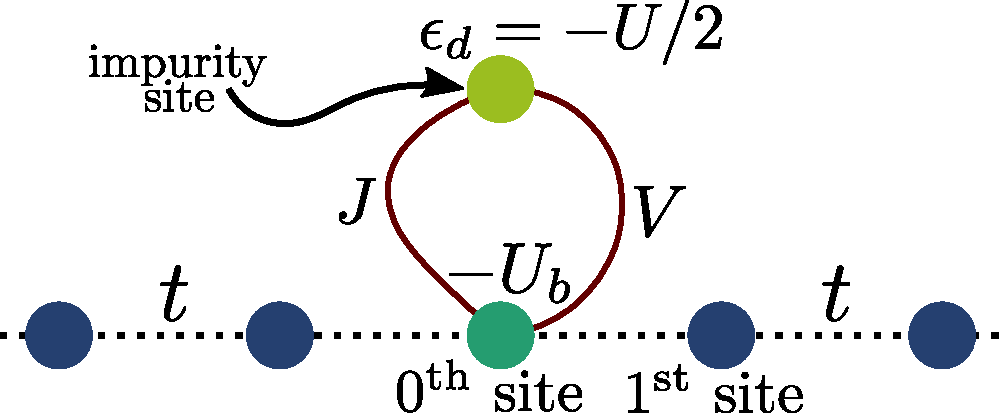
\includegraphics[width=0.95\textwidth]{figures/gen_siam.pdf}
\end{minipage}

\footcite{Schrieffer_Wolff,anderson_impurity_1961}

\end{frame}

\section{URG Analysis: \(U_b=0\)}
\begin{frame}[noframenumbering]{\(U_b = 0:\) Flow towards strong-coupling}
\centering
% \vspace*{-10pt}
{\(\mathbf{U > 0, J > 0}\)}

\vspace*{10pt}

\only<+>{
\hspace*{-50pt}
\begin{minipage}{0.6\textwidth}
\centering
{\Large \(d_0 = \omega - \frac{D}{2} - \frac{U}{2} + \frac{K}{4}, \quad d_1 = \omega - \frac{D}{2} + \frac{U}{2} + \frac{J}{4}\)\\[1pt]
\(d_2 = \omega - \frac{D}{2} + \frac{J}{4}\)}
\end{minipage}
\hspace*{20pt}
\begin{minipage}{0.38\textwidth}
\centering
{\Large \(\Delta V = \frac{3n_j VJ}{8}\left(\frac{1}{|d_2|} + \frac{1}{|d_1|}\right) > 0\)\\[5pt]
\(\Delta J = \frac{n_j J^2}{|d_2|} > 0\)}
\end{minipage}
\hspace*{-50pt}

	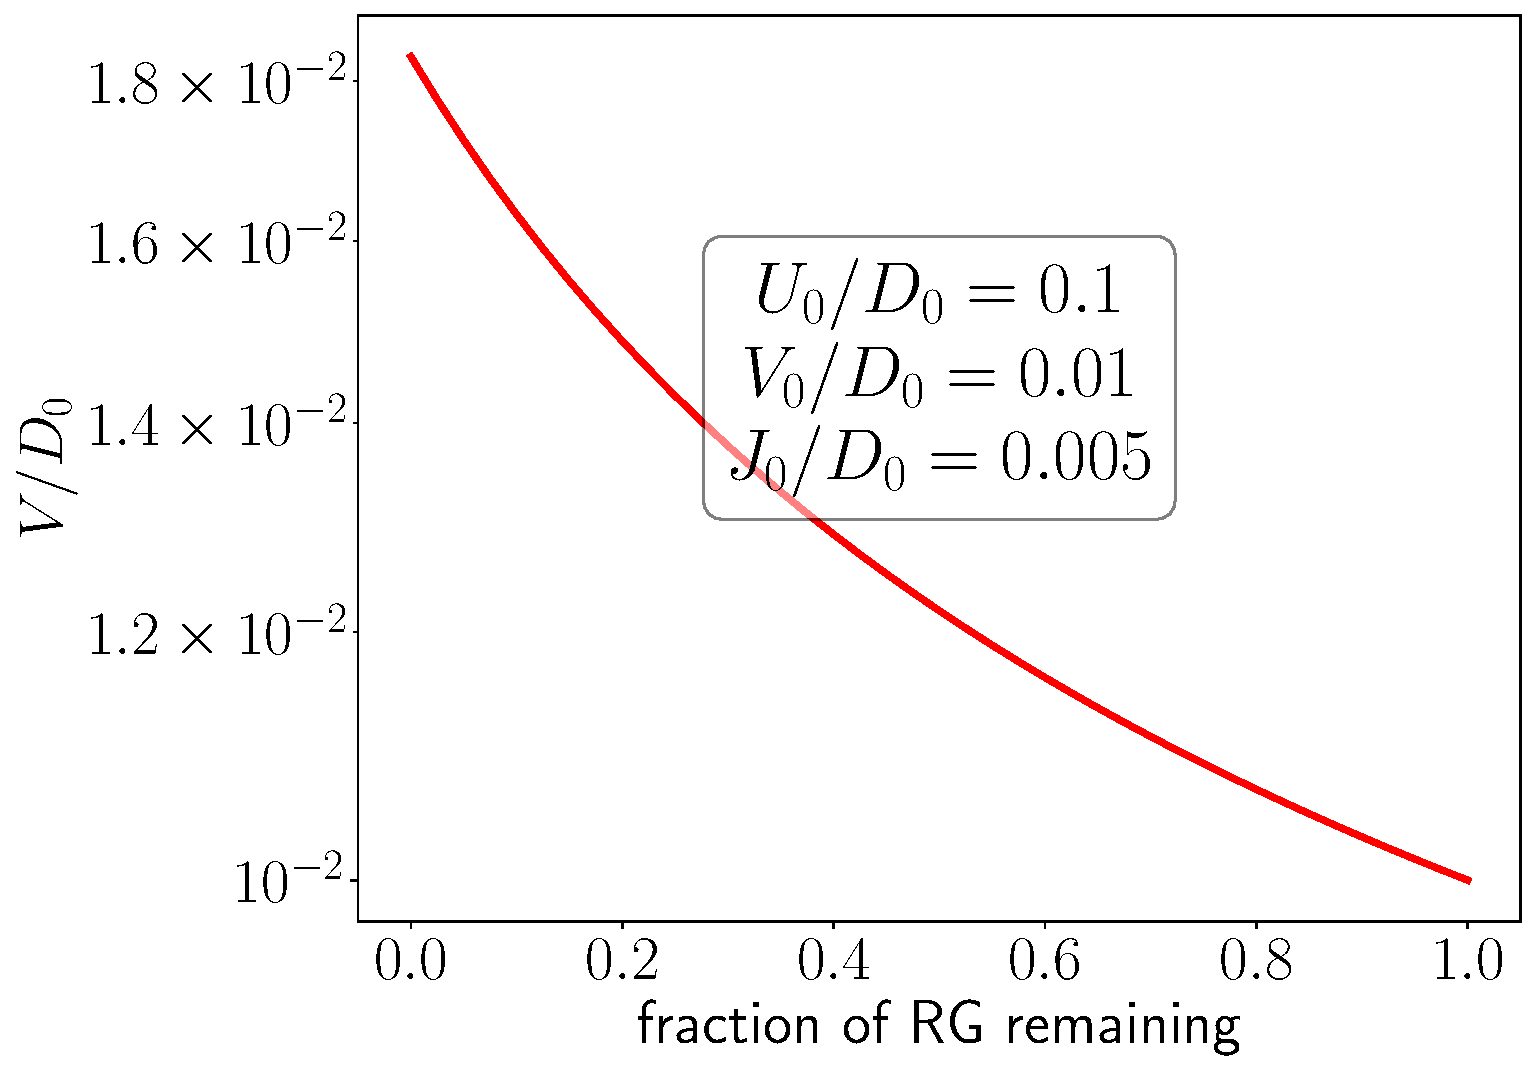
\includegraphics[width=0.49\textwidth]{figures/U_irr,U>0,V.pdf}
	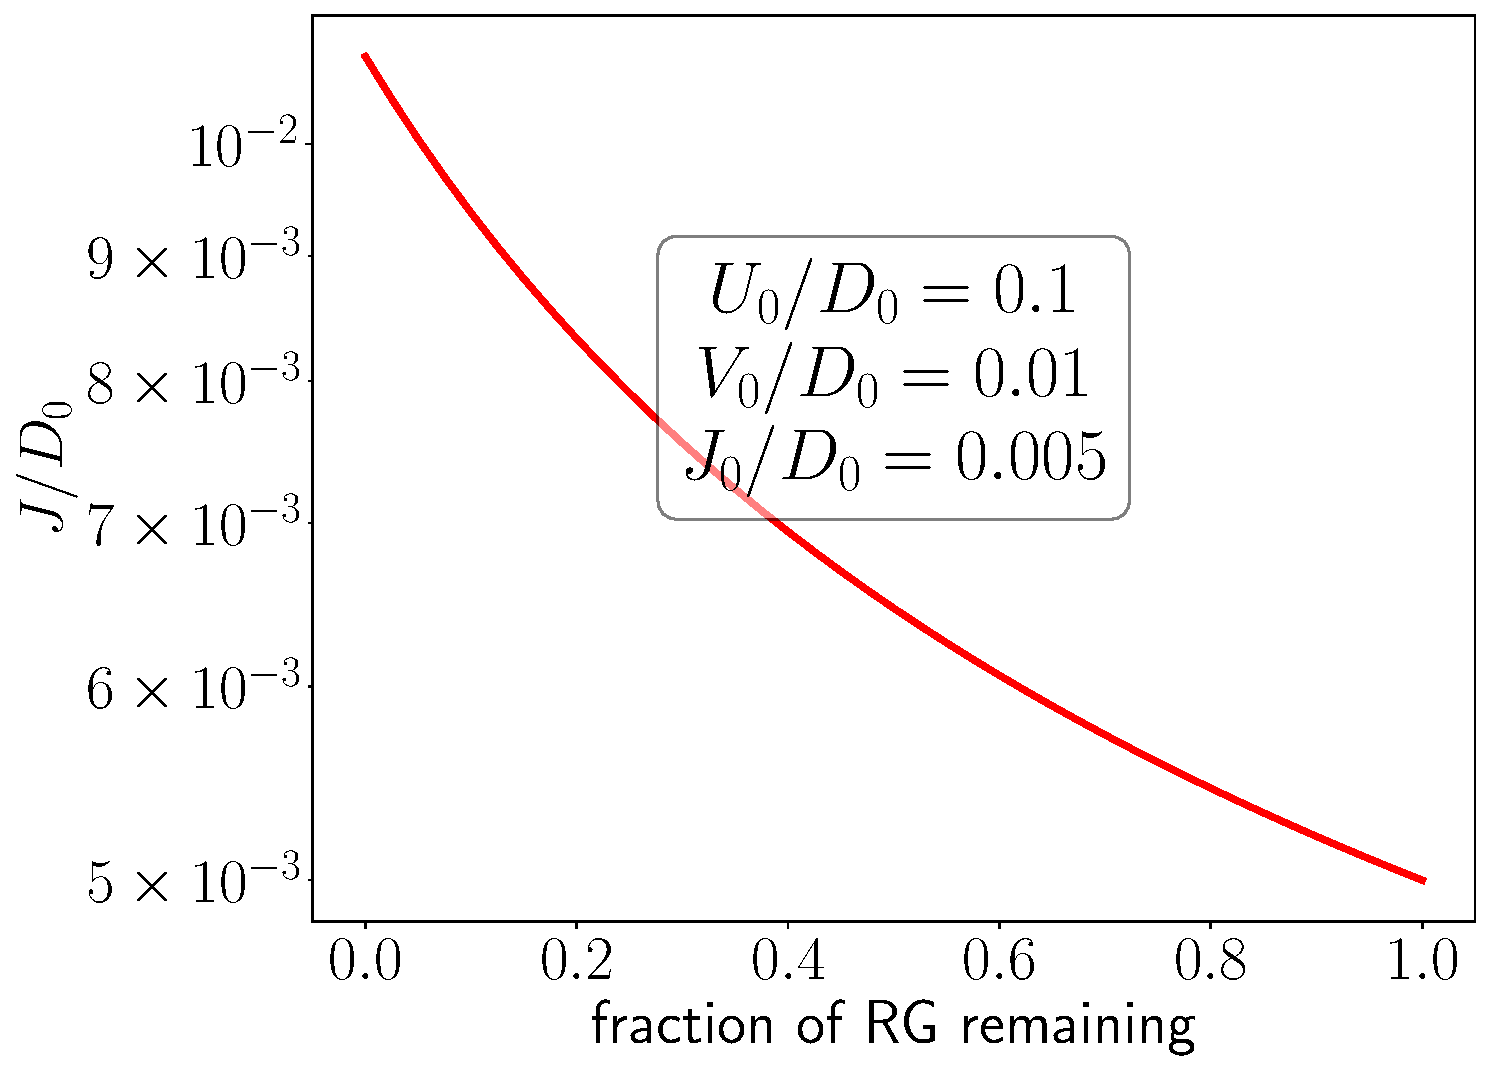
\includegraphics[width=0.49\textwidth]{figures/U_irr,U>0,J.pdf}
}
\only<+>{
{\Large \(\Delta U = 4V^2 n_j\left(\frac{1}{d_1} - \frac{1}{d_0}\right) - n_j\frac{J^2}{d_2}\)}

% \vspace*{-10pt}

\begin{minipage}{0.49\textwidth}
\centering
{\large\( V > J\)}

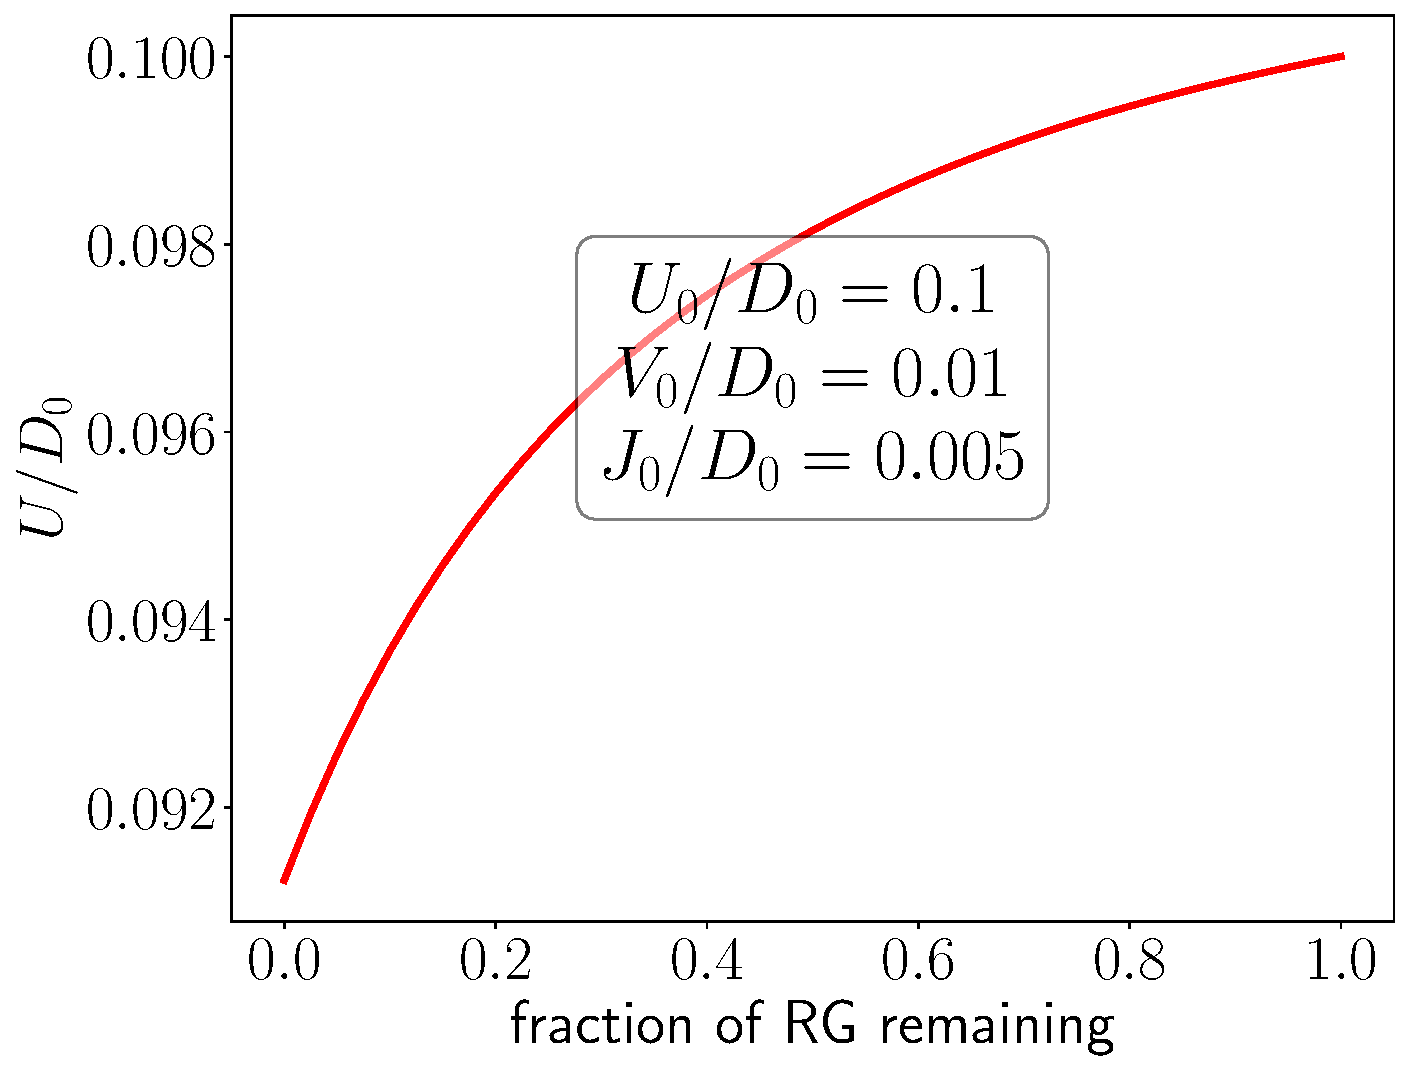
\includegraphics[width=\textwidth]{figures/U_irr,U>0,U.pdf}
\end{minipage}
\begin{minipage}{0.49\textwidth}
\centering
{\large\( V < J\)}

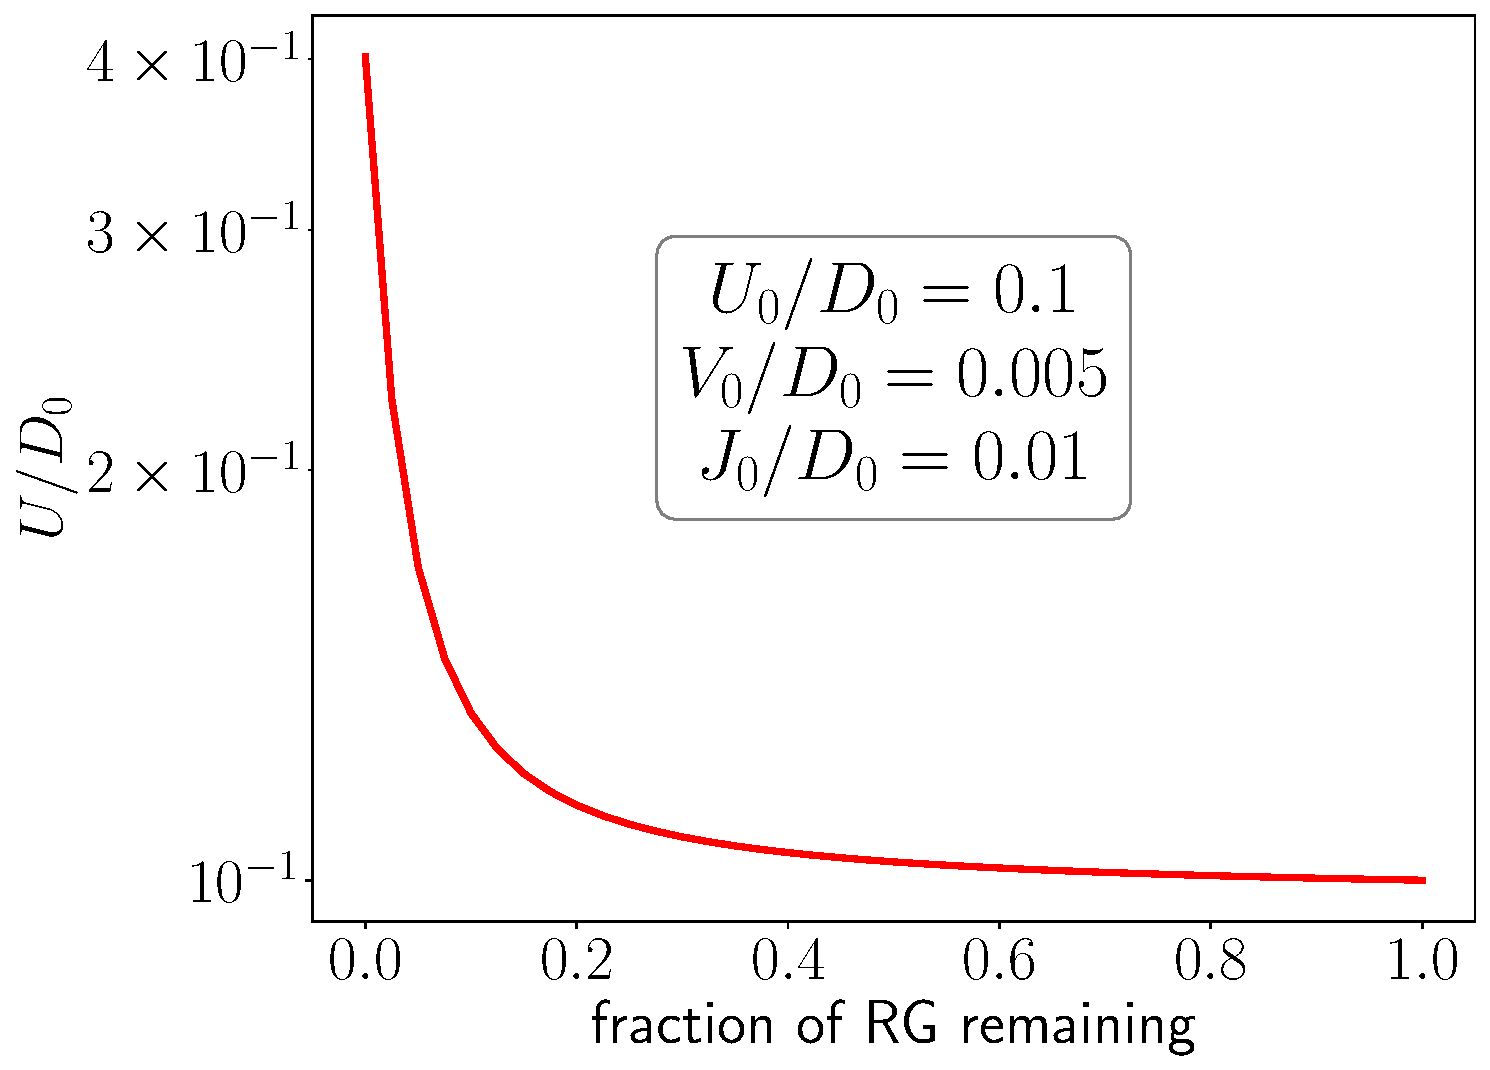
\includegraphics[width=\textwidth]{figures/U_rel,U>0,U.pdf}
\end{minipage}
}

\end{frame}

\begin{frame}[noframenumbering]{\(U > 0\) Fixed point Hamiltonian}
\begin{minipage}{0.48\textwidth}
	\[H^* = \sum_{k < k^*,\sigma}\epsilon_{k}\hat{n}_{k\sigma} ~ + \frac{U^*}{2}\left(\hat n_{d \uparrow} - \hat n_{d \downarrow}\right)^2 ~ + J^* \vec{S}_d\cdot \vec{s}_<\]
	\[+ ~ V^* \sum_{k < k^*,\sigma}\left(c^\dagger_{d\sigma}c_{k\sigma} + \text{h.c.}\right)\]

	\vspace*{20pt}
	\[\vec{s}_< = \frac{1}{2}\sum_{k,k^\prime < k^*}c^{\dagger}_{k\alpha}\vec{\sigma}_{\alpha\beta}c_{k^\prime,\beta}\]
\end{minipage}
\begin{minipage}{0.5\textwidth}
	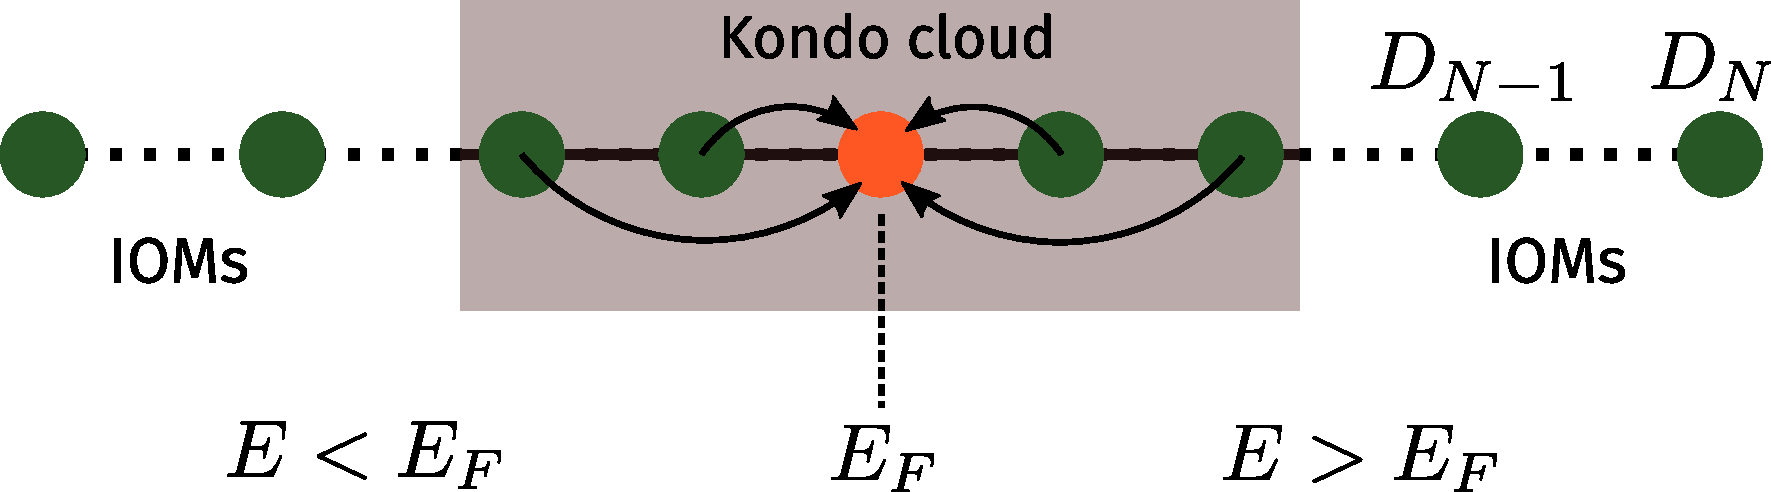
\includegraphics[width=\textwidth]{figures/kondo_fp_1D.pdf}
\end{minipage}
\end{frame}

\begin{frame}[noframenumbering]{Impurity Spectral Function}
\centering
\hspace*{-15pt}
\begin{minipage}{0.25\textwidth}
\focus{no gap} at arbitrarily large $U$
\end{minipage}
\hspace*{25pt}
\begin{minipage}{0.7\textwidth}
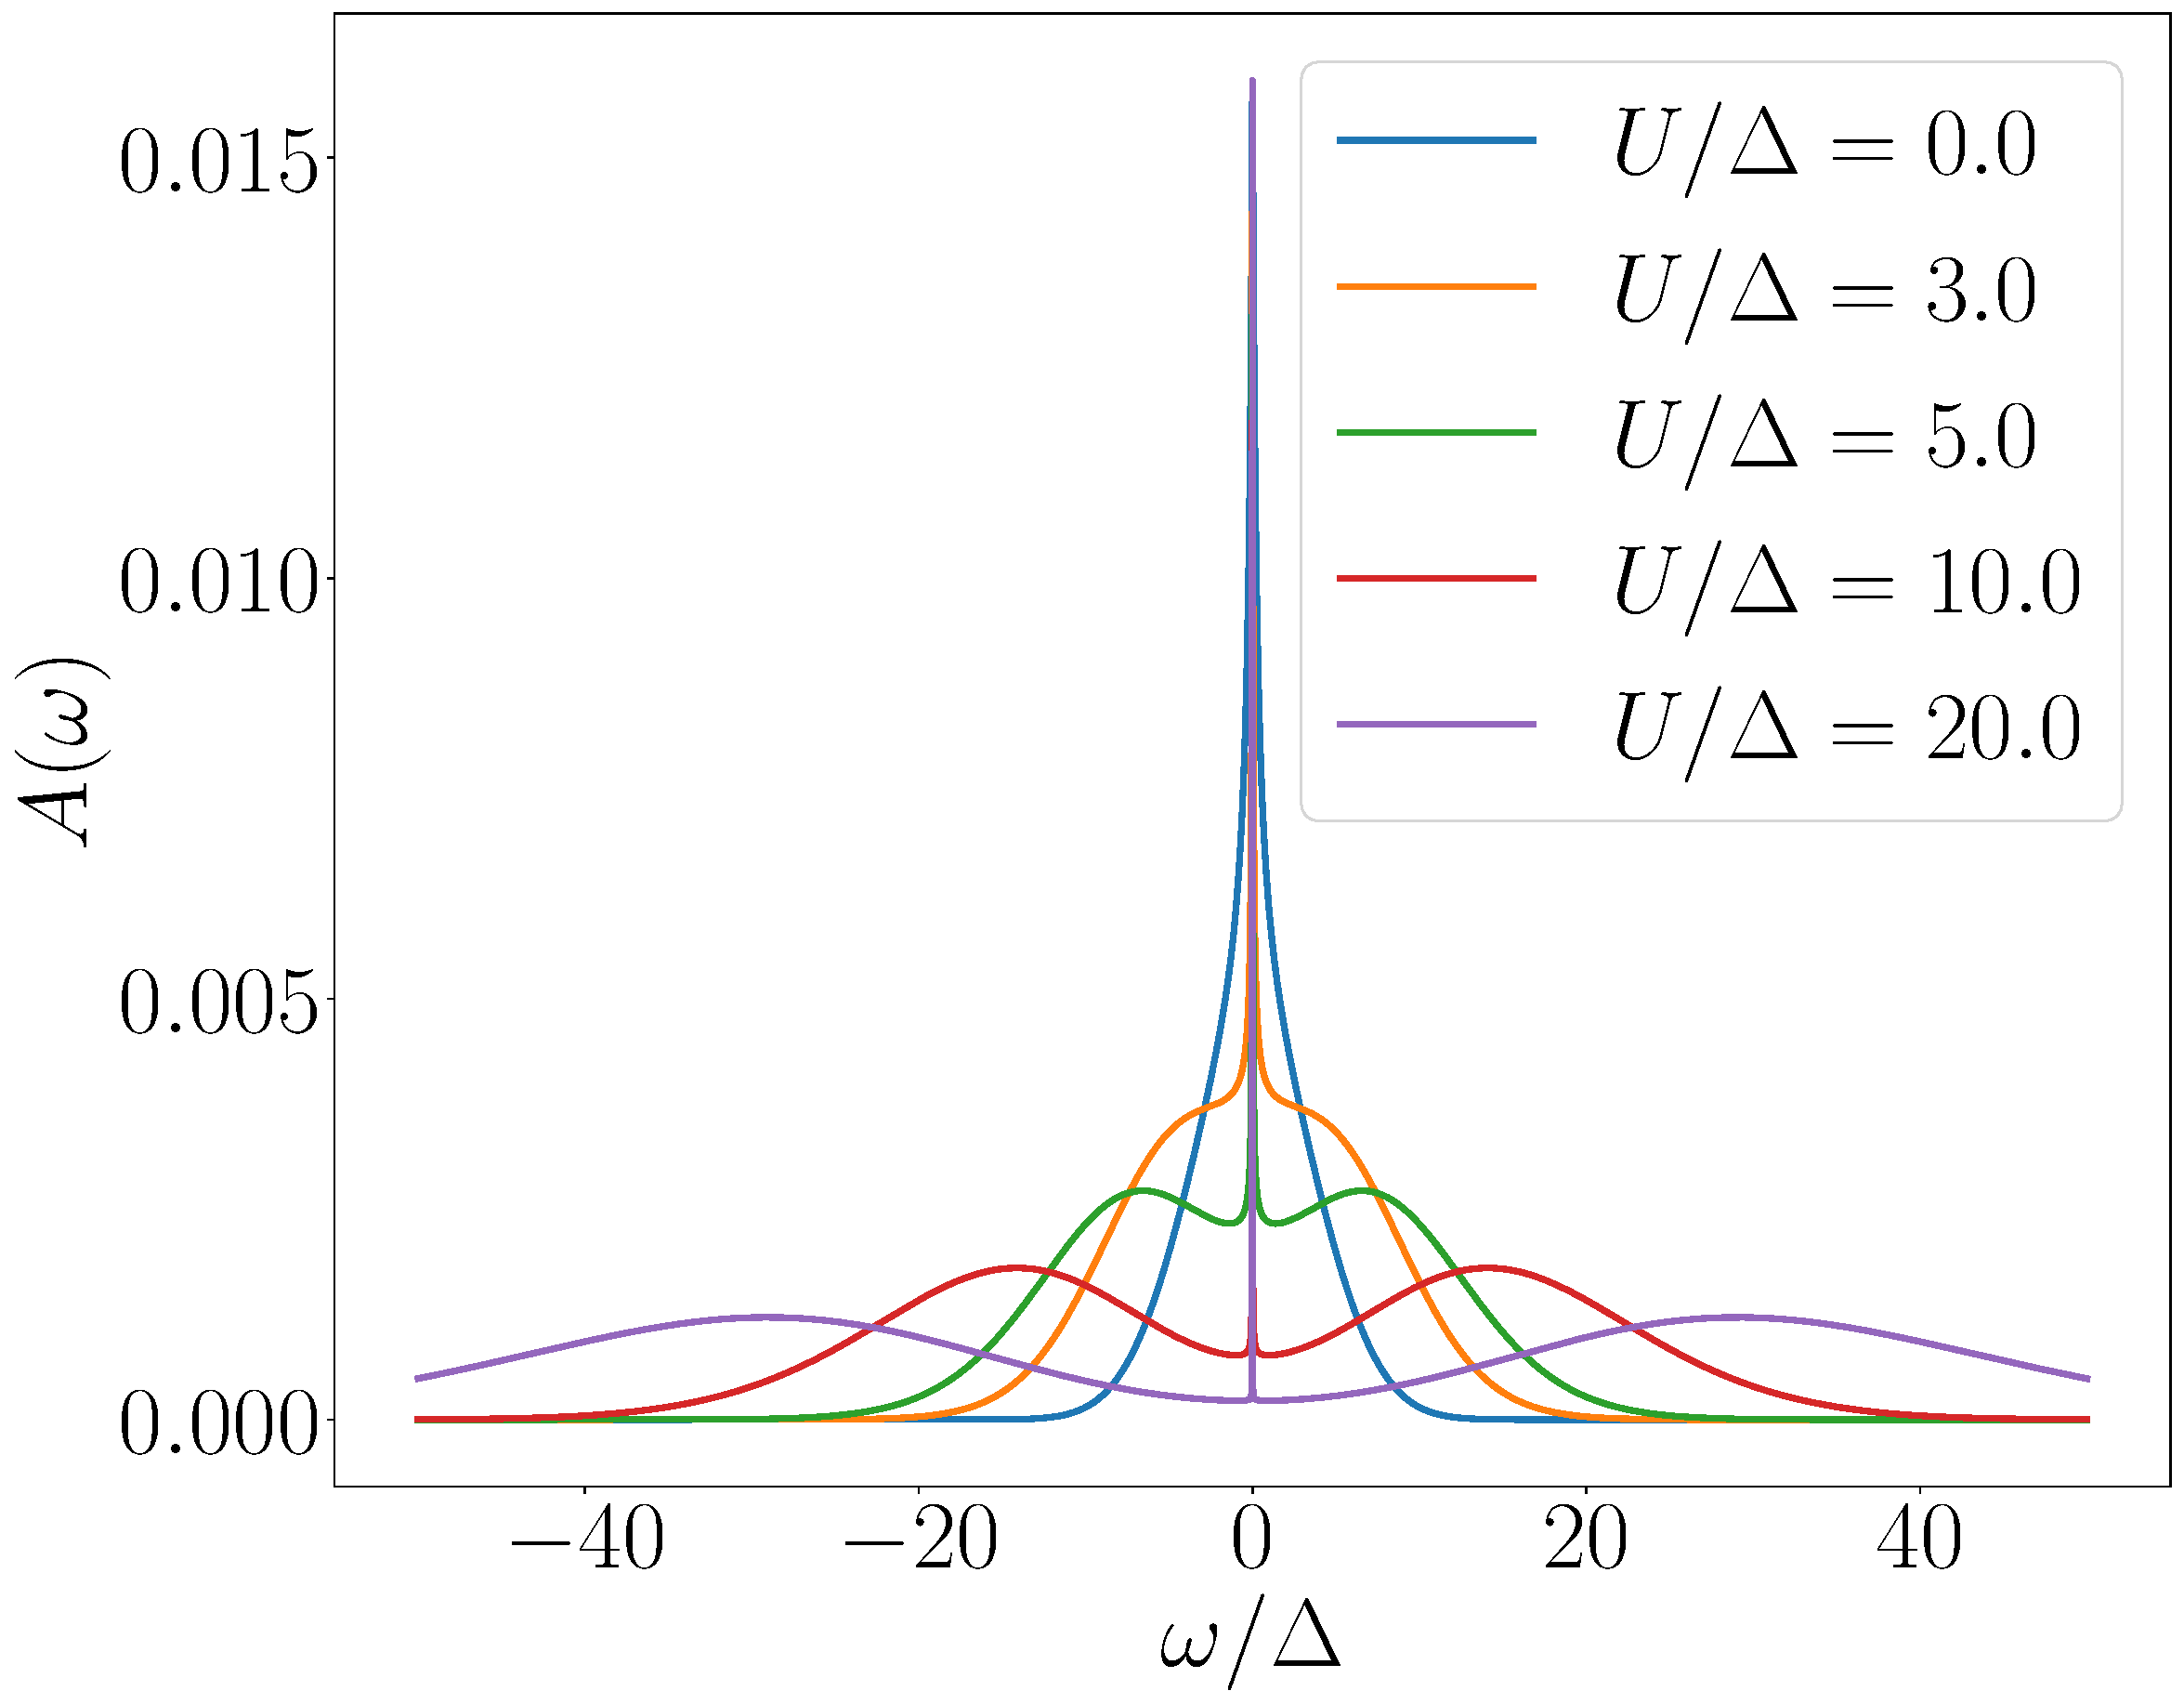
\includegraphics[width=\textwidth]{./figures/gen_siam_spec_func.pdf}
\hspace*{-25pt}
\end{minipage}
\end{frame}

\section{URG Analysis: \(U_b \neq 0\)}

\begin{frame}[noframenumbering]{\(U > 0\) RG Equations}

\begin{itemize}
	\item \(U_b\) is \focus{marginal}: ~ ~ ~\(\Delta U_b = 0\)
	\item Spin-exchange couling \(J\) can now be \focus{driven irrelevant} by \(U_b\): 
	\begin{equation*}
	\Delta J = -\frac{n_j J\left(J + 4U_b\right)}{d_2} \longrightarrow \begin{cases}
	\text{\textcolor{blue}{relevant} when }J+4U_b > 0\\
	\text{\textcolor{red}{irrelevant} when }J+4U_b < 0\\
	\end{cases}
	\end{equation*}
	\item Same can be said for the hybridisation \(V\):
	\begin{equation*}
	\Delta V = -\frac{3n_j V}{8}\left[\left(J + \frac{4U_b}{3}\right) \left(\frac{1}{d_2} + \frac{1}{d_1}\right) + \frac{4U_b}{3}\left(\frac{1}{d_3} + \frac{1}{d_0}\right)\right] \longrightarrow \begin{cases}
	\text{\textcolor{blue}{rel.} when }J+4U_b > 0\\
	\text{\textcolor{red}{irrel.} when }J+4U_b < 0\\
	\end{cases}
	\end{equation*}
	\item \focus{\(U\) can be relevant if \(J\) decays slower than \(V\)}; needs to be checked numerically
\end{itemize}
\end{frame}

\begin{frame}[noframenumbering]{\(U > 0\) Phase Diagram}
\hspace*{-20pt}
\begin{minipage}{0.5\textwidth}
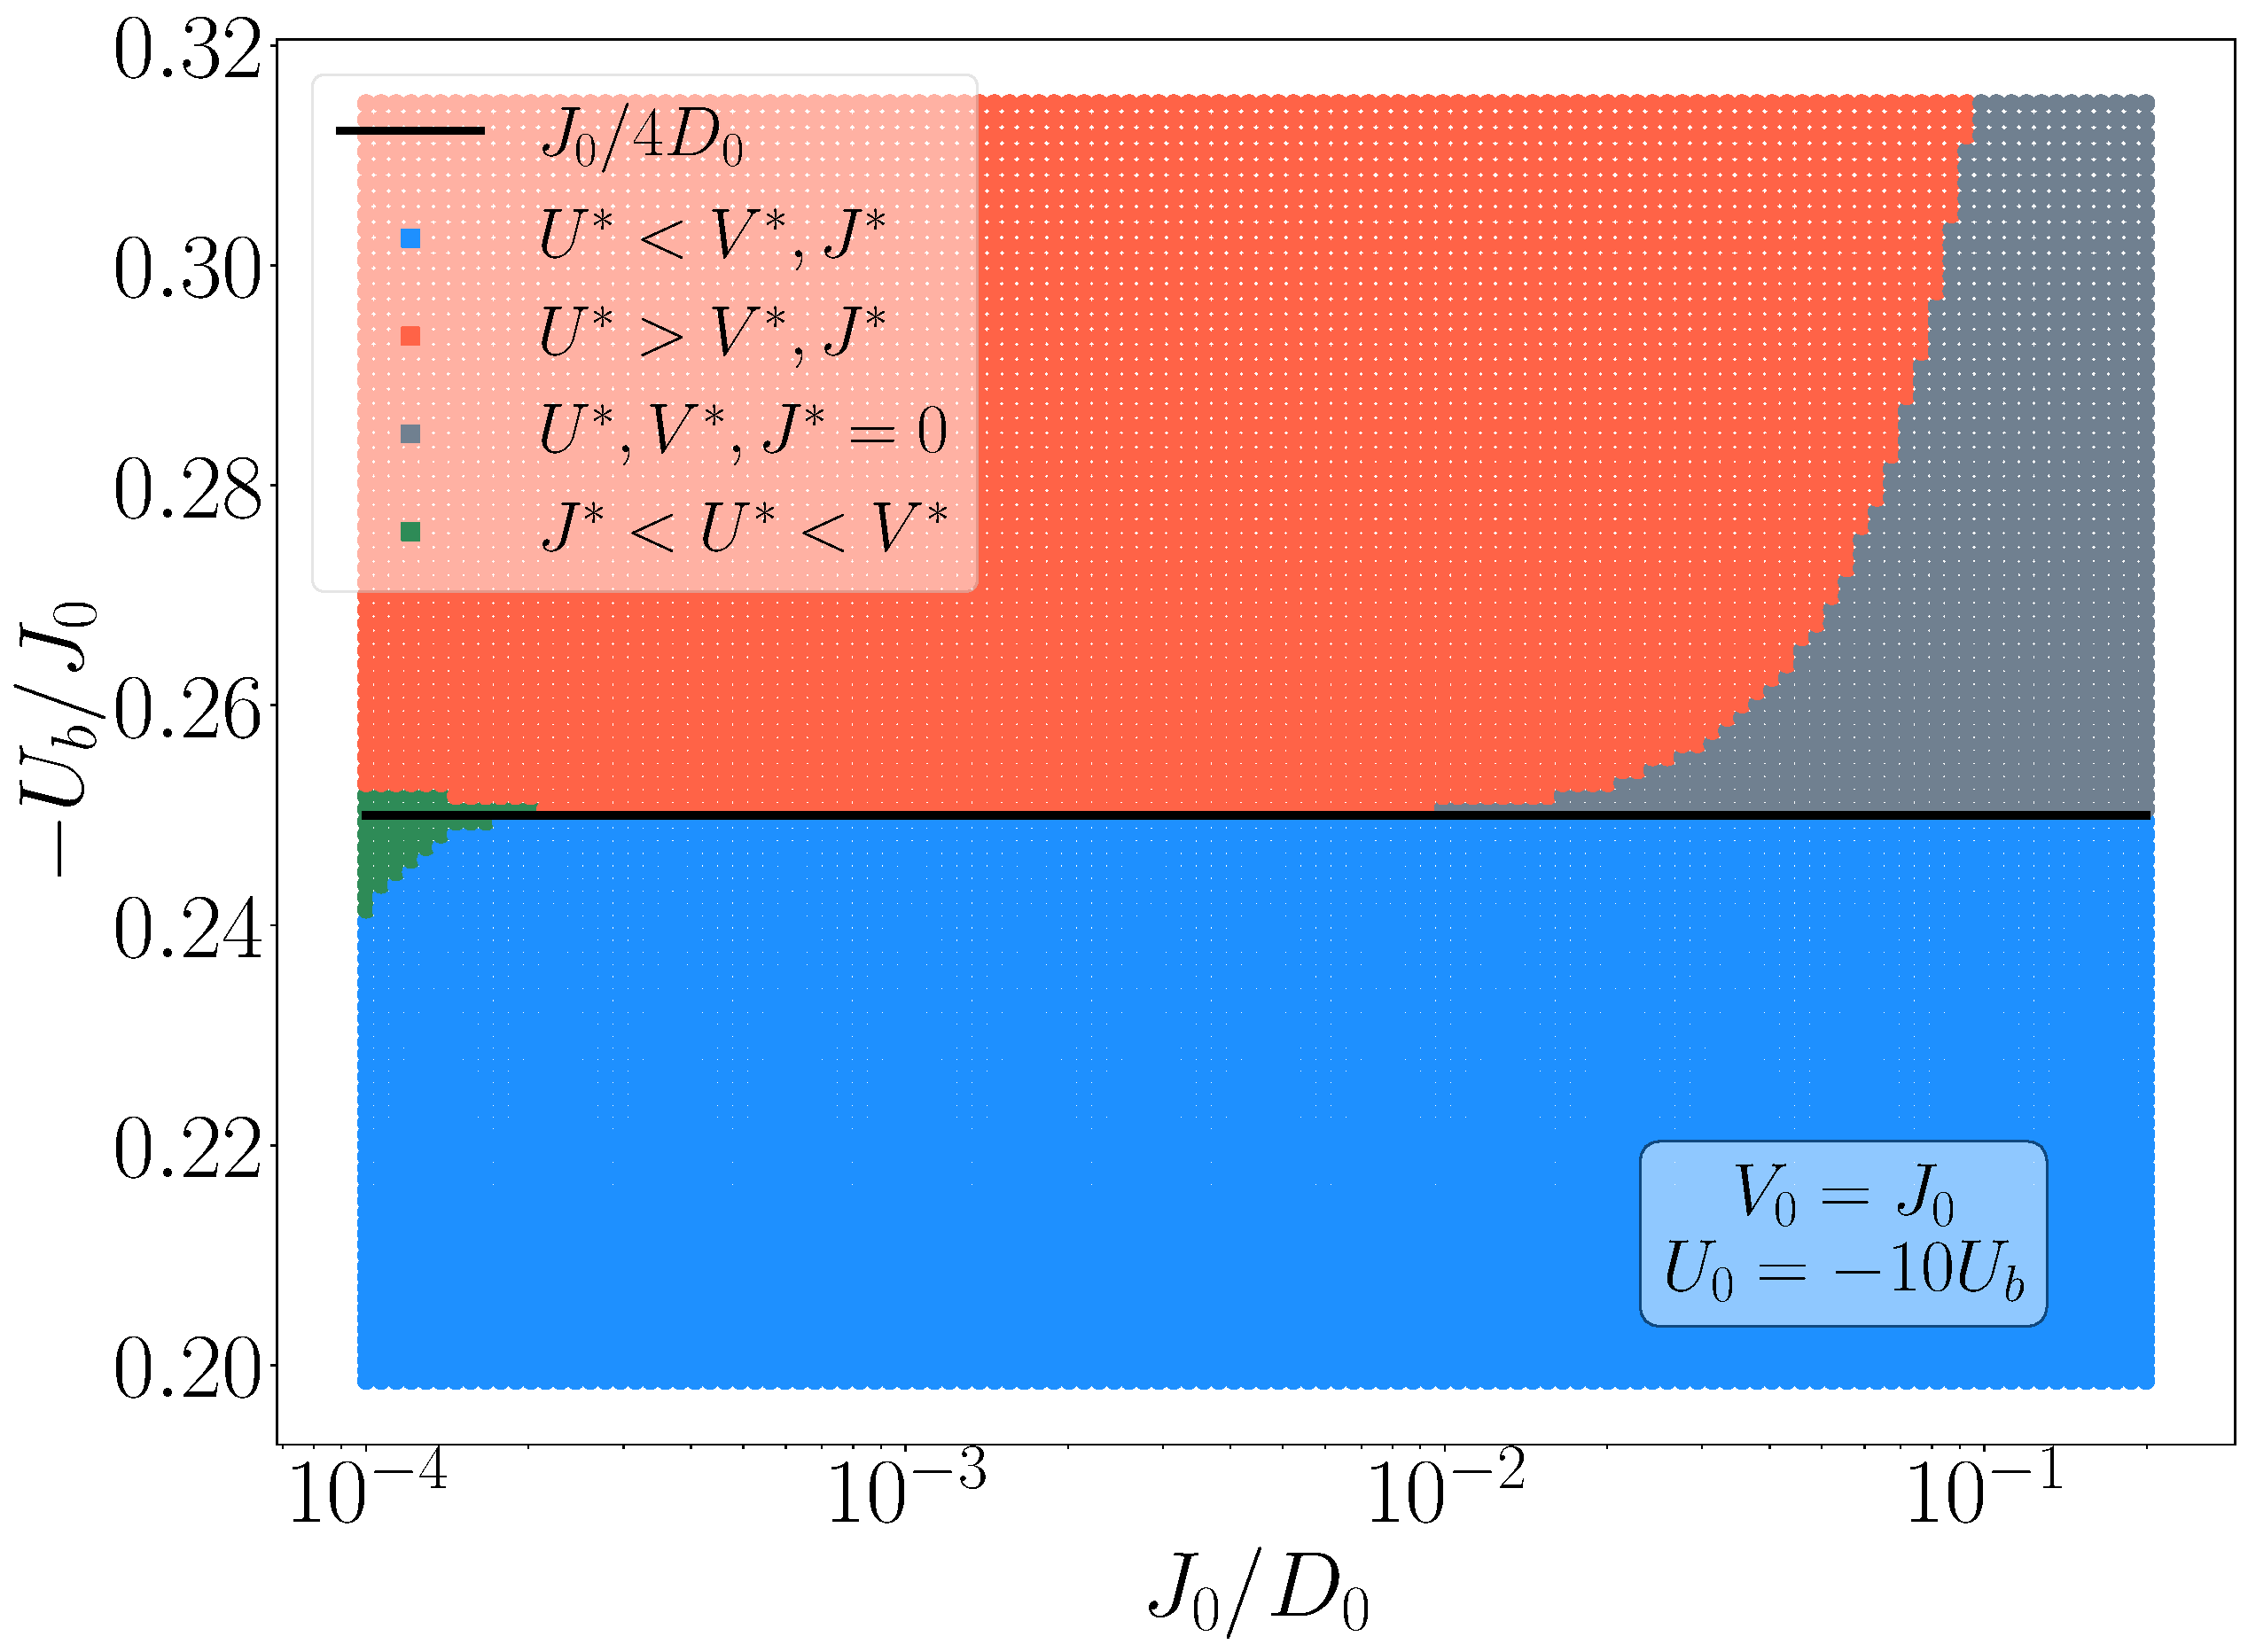
\includegraphics[width=\textwidth]{./figures/phase-map-MIT.pdf}
\end{minipage}
\begin{minipage}{0.53\textwidth}
	\begin{itemize}
	\item black line represents line of \focus{critical points} at \(U_b^* = -J^*/4\)
	\item blue: screened impurity (strong-coup.)\\[10pt]
	\item red: unscreened local mom. (\(J=V=0\))\\[10pt]
	\item gray: imp. level absent (\(U=J=V=0\))\\[10pt]
	\item green: \(J\) vanishes (\(J < U\)) (this region vanishes in therm. limit)
	\end{itemize}
\end{minipage}

\begin{center}
\hspace*{-20pt}
{\small
\begin{tabular}{|c|c|c|c|c|}
\hline
phase & RG flow & fixed point & GS & 2-site GS \\ 
\hline
blue & \(\Delta U <0, \Delta J,\Delta V>0\) & \(U^* \ll V^* \ll J^*\) & SS & \(\ket{SS}=\ket{\uparrow,\downarrow} - \ket{\downarrow, \uparrow}\)  \\ 
green &  \(\Delta U < 0, \Delta J < 0,\Delta V>0\) & \(J^* < U^* \ll V^*\) & SS + CT-0 & \(c\ket{SS} + \sqrt{1-c^2}\ket{CT-0}\)  \\  
red &  \(\Delta U > 0, \Delta J,\Delta V<0\) & \(U^* \gg 1,  V^* = J^* = 0\) & loc. mom & \(\left\{\ket{\uparrow}, \ket{\downarrow} \right\} \otimes \left\{\ket{0}, \ket{2}\right\} \) \\
gray &  \(\Delta U, \Delta J,\Delta V < 0\) & \(U^* = V^* = J^* = 0\) & bath & \(\left\{\ket{\uparrow}, \ket{\downarrow}, \ket{0}, \ket{2} \right\} \otimes \left\{\ket{0}, \ket{2}\right\}\) \\
\hline
\end{tabular}
}
\end{center}
\end{frame}

\section{Evolution of two-site groundstate and correlations across the transition}

\begin{frame}[noframenumbering]{Overlap of ground state against spin singlet and charge triplet zero states}
	\centering
\only<1>{\(J_0/D_0 = 10^{-4}\)

\vspace*{-20pt}
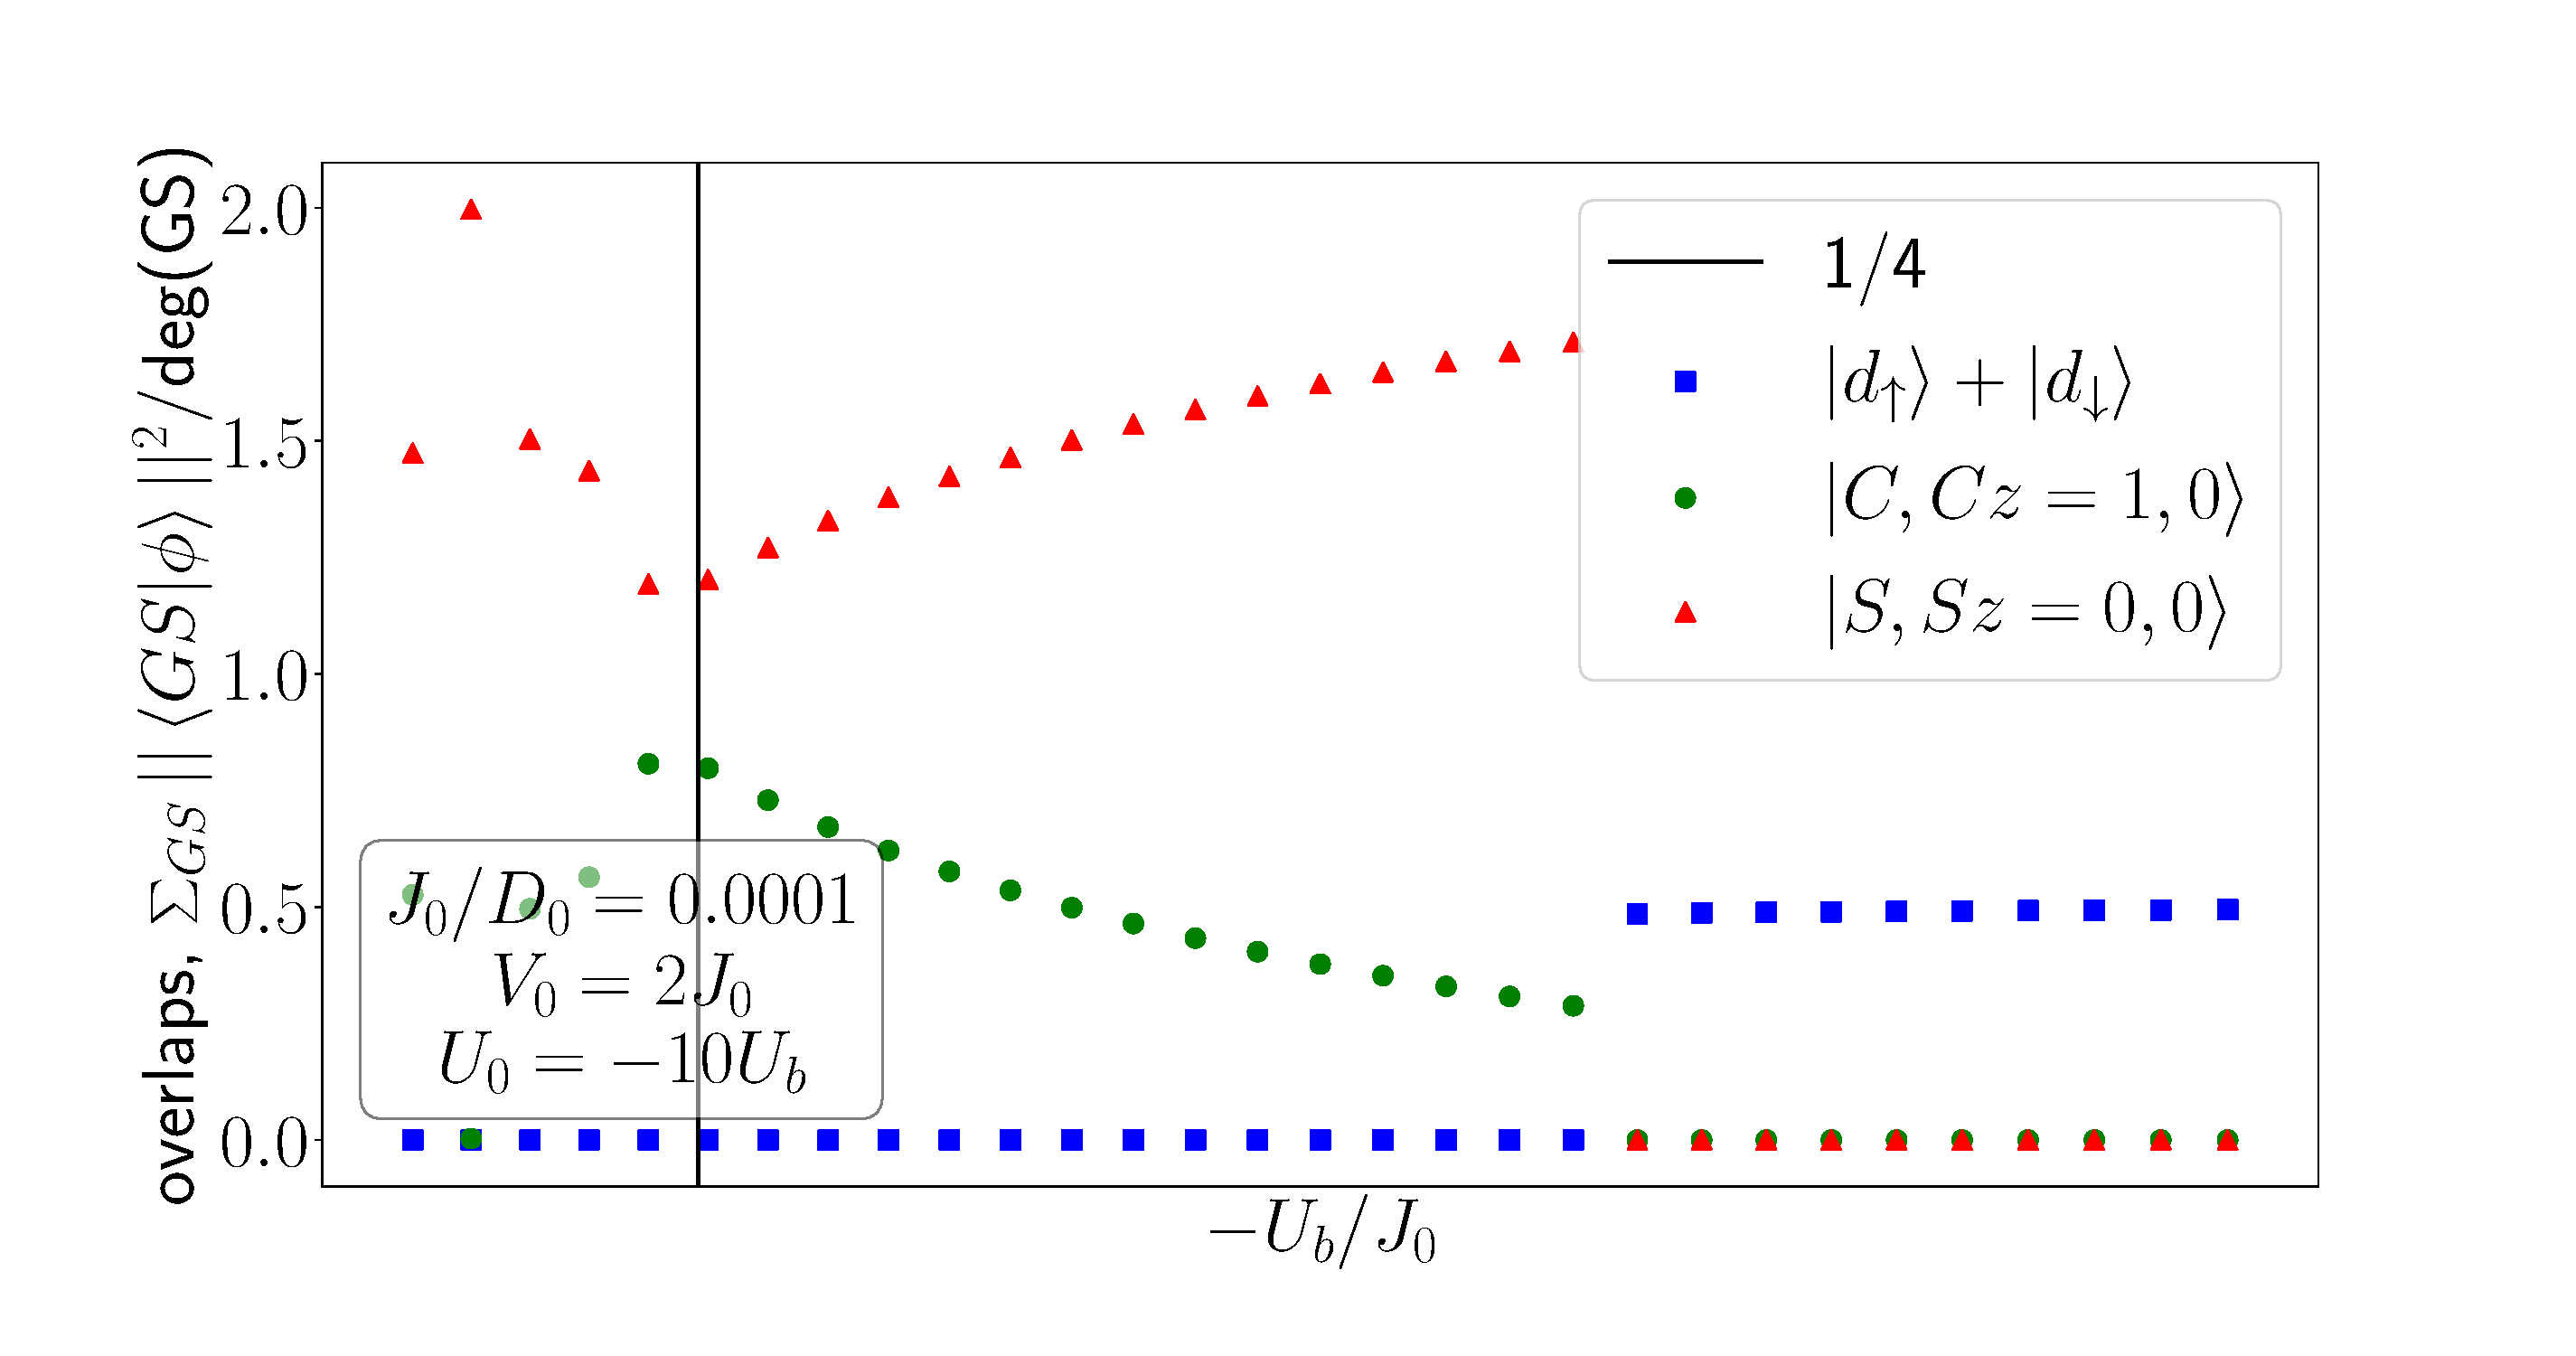
\includegraphics[width=\textwidth]{./figures/overlaps_gs-J=0.100.pdf}
}

\only<2>{\(J_0/D_0 = 10^{-2}\)

\vspace*{-20pt}
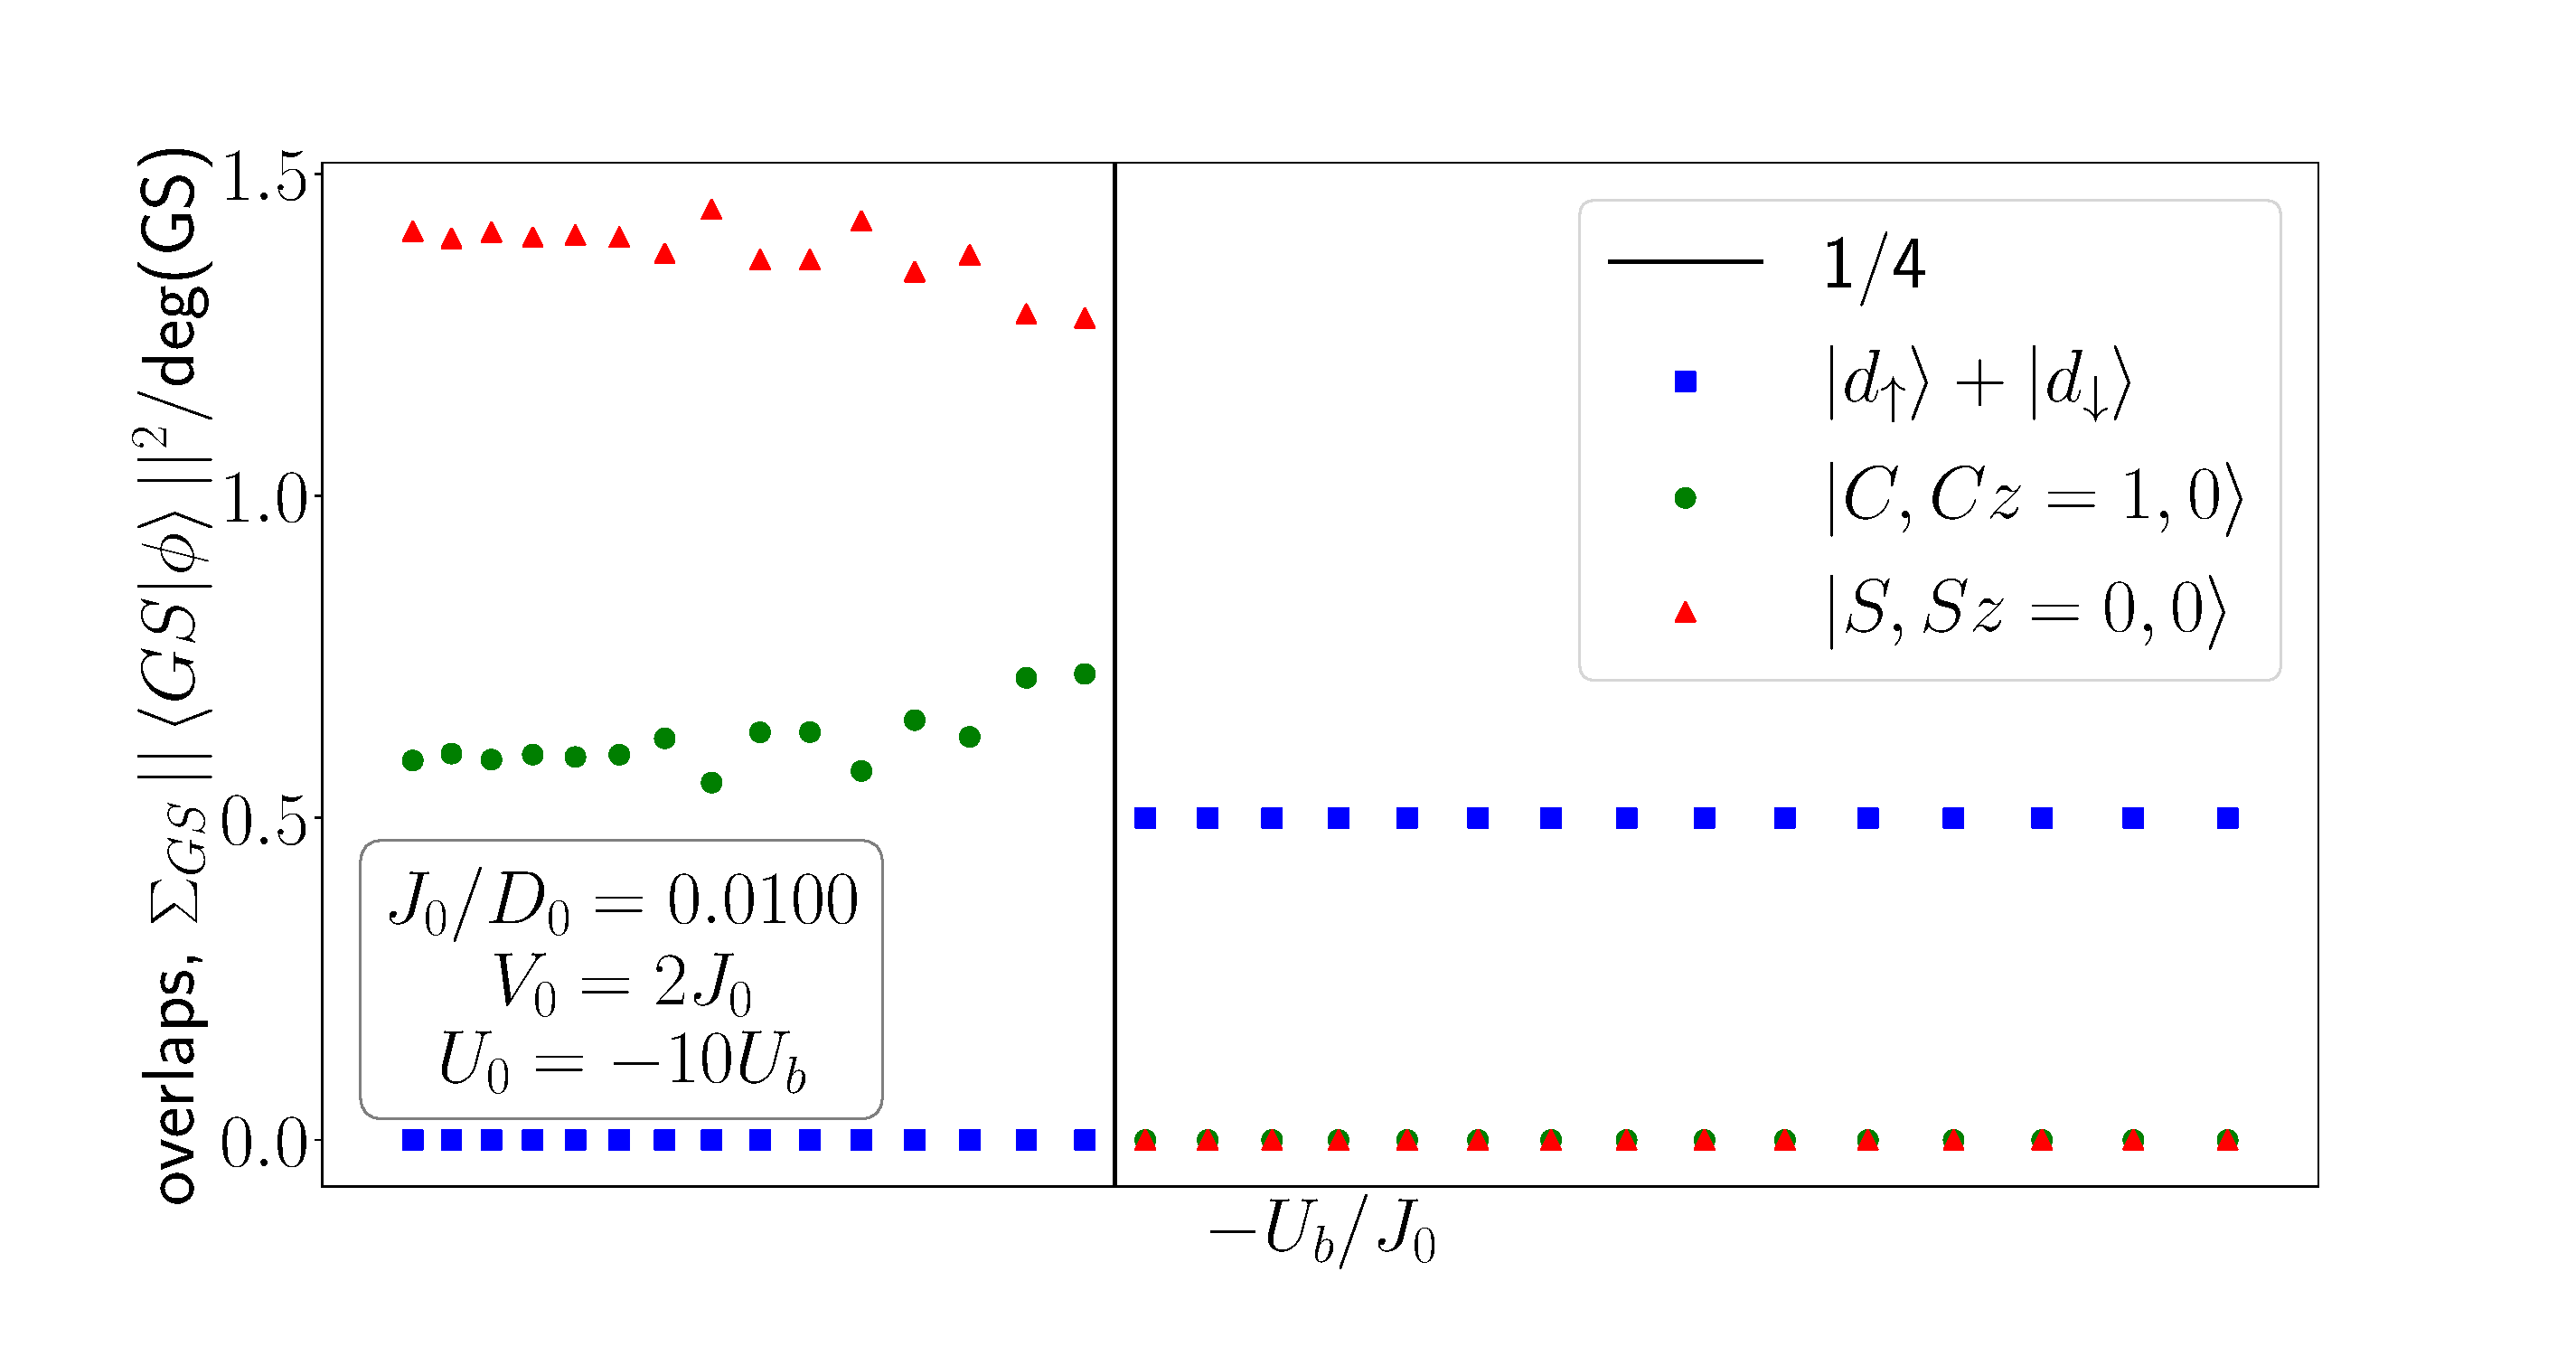
\includegraphics[width=\textwidth]{./figures/overlaps_gs-J=10.000.pdf}}

\only<3>{\(J_0/D_0 = 10^{-1}\)

\vspace*{-20pt}
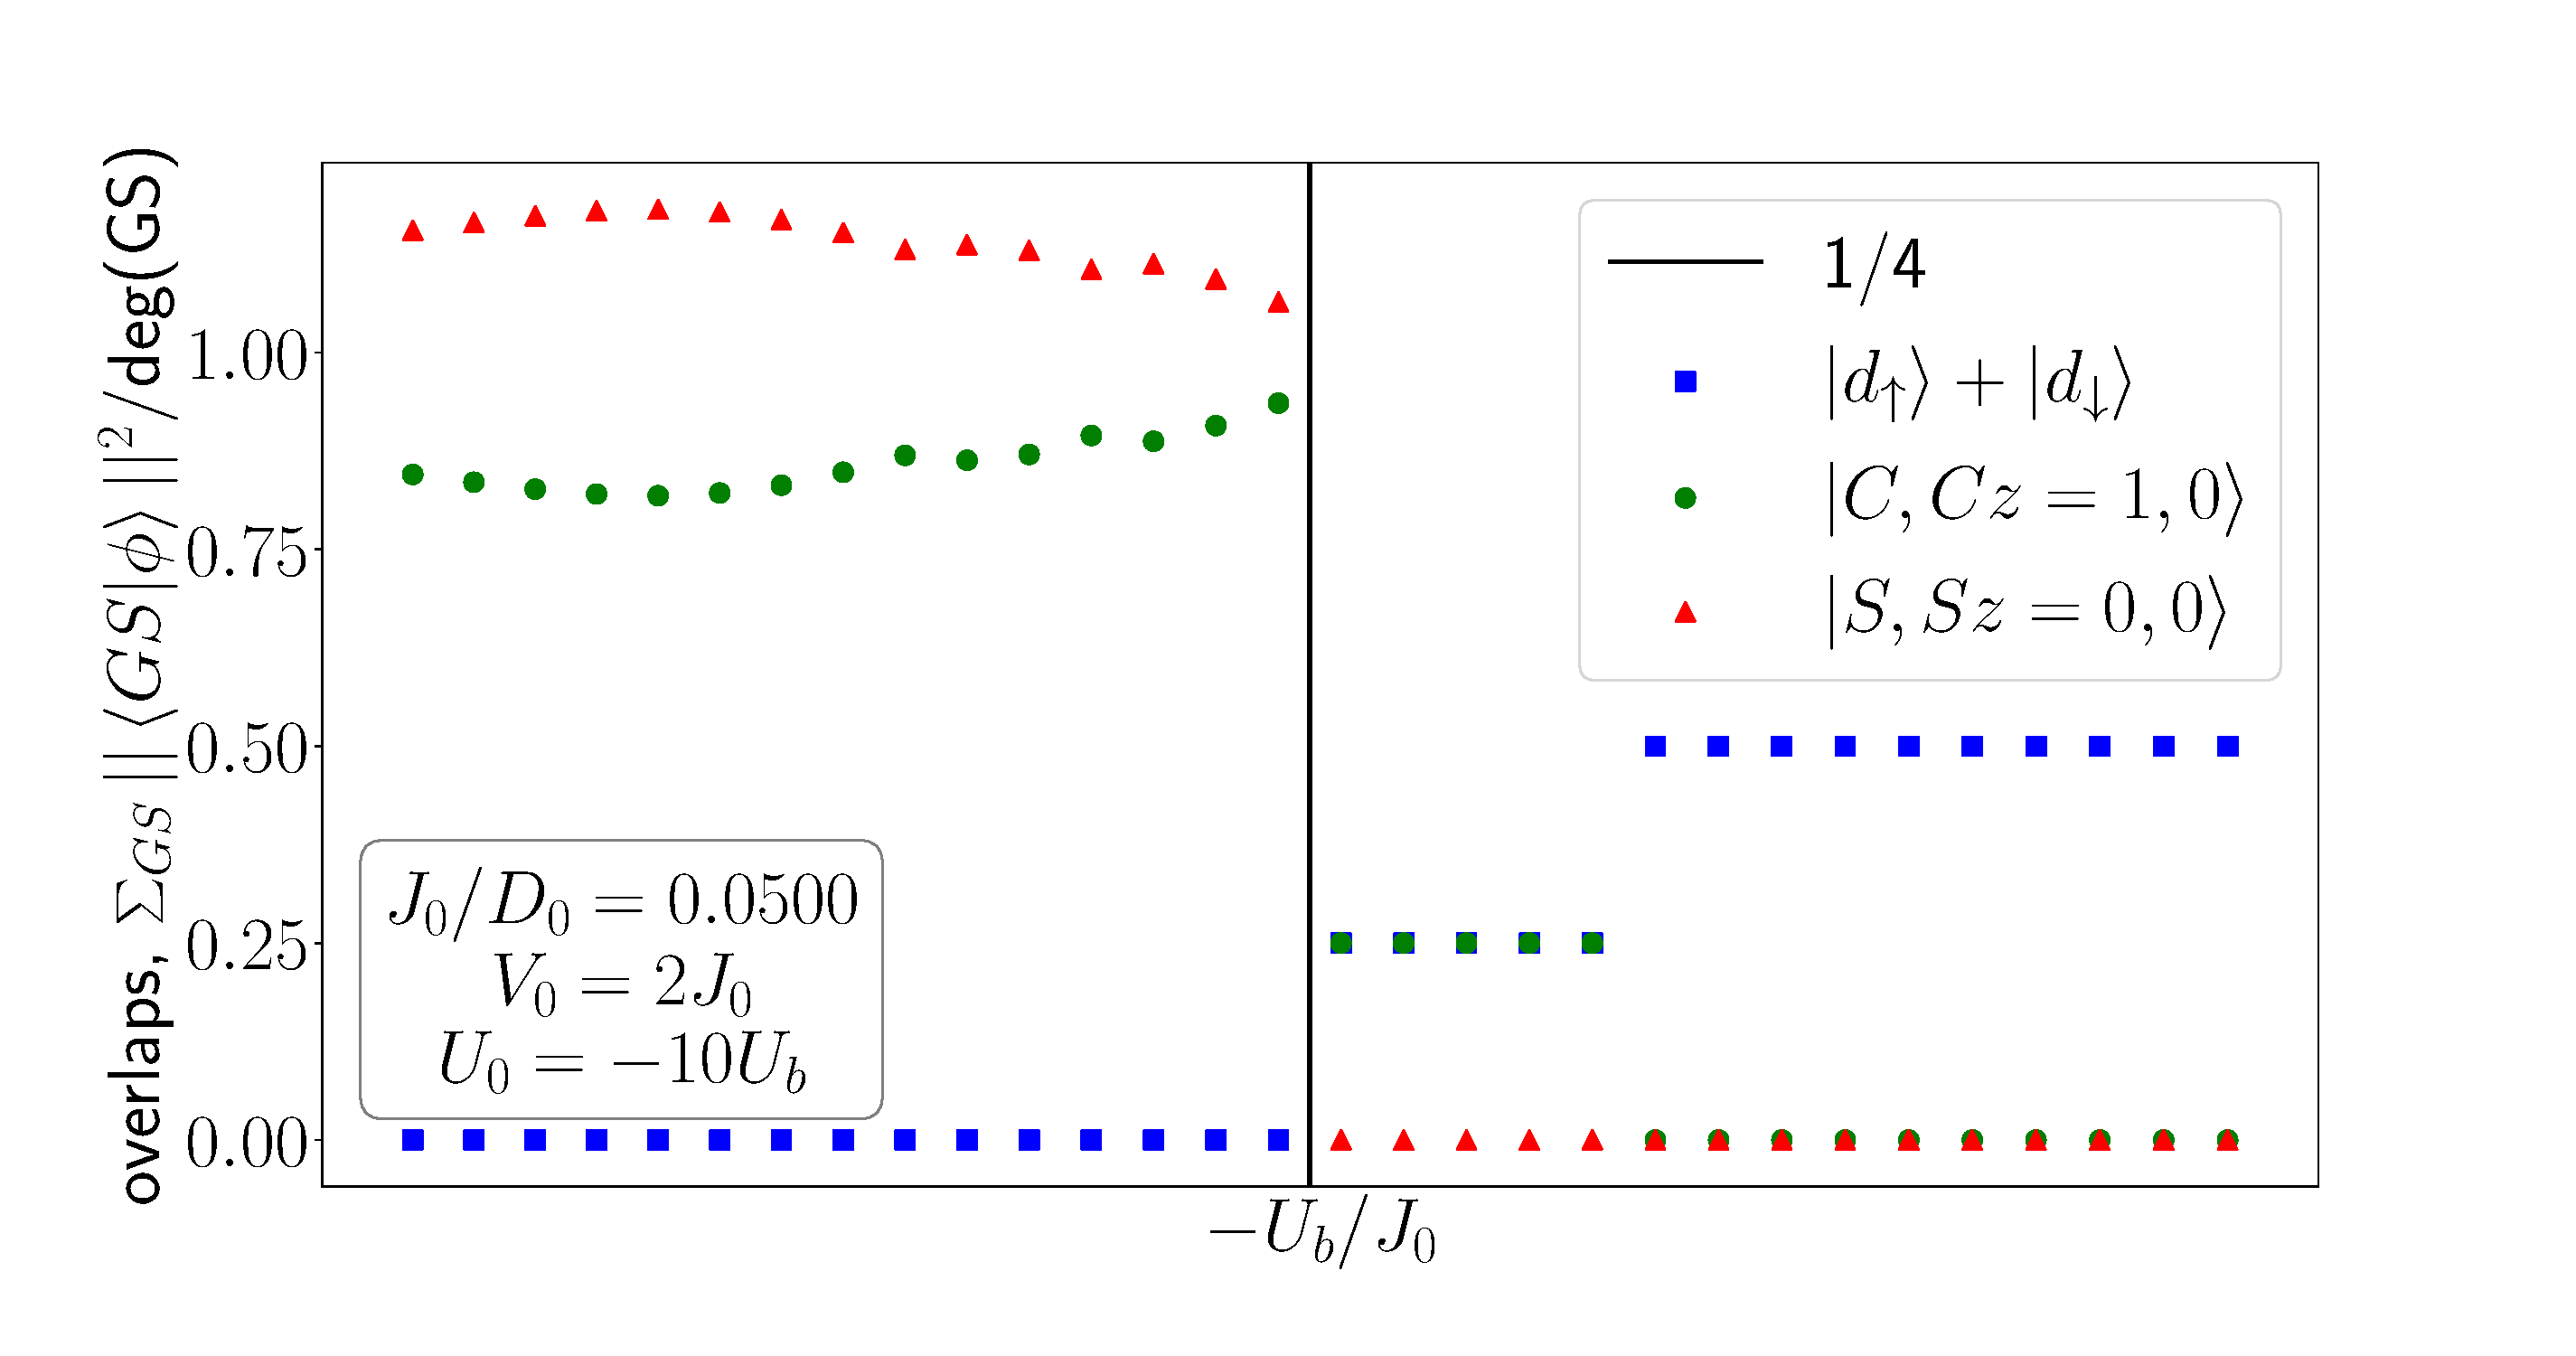
\includegraphics[width=\textwidth]{./figures/overlaps_gs-J=50.000.pdf}}

\end{frame}

\begin{frame}[noframenumbering]{Spin and charge correlations in ground state}
	\centering
\only<1>{\(J_0/D_0 = 10^{-4}\)

\vspace*{-20pt}
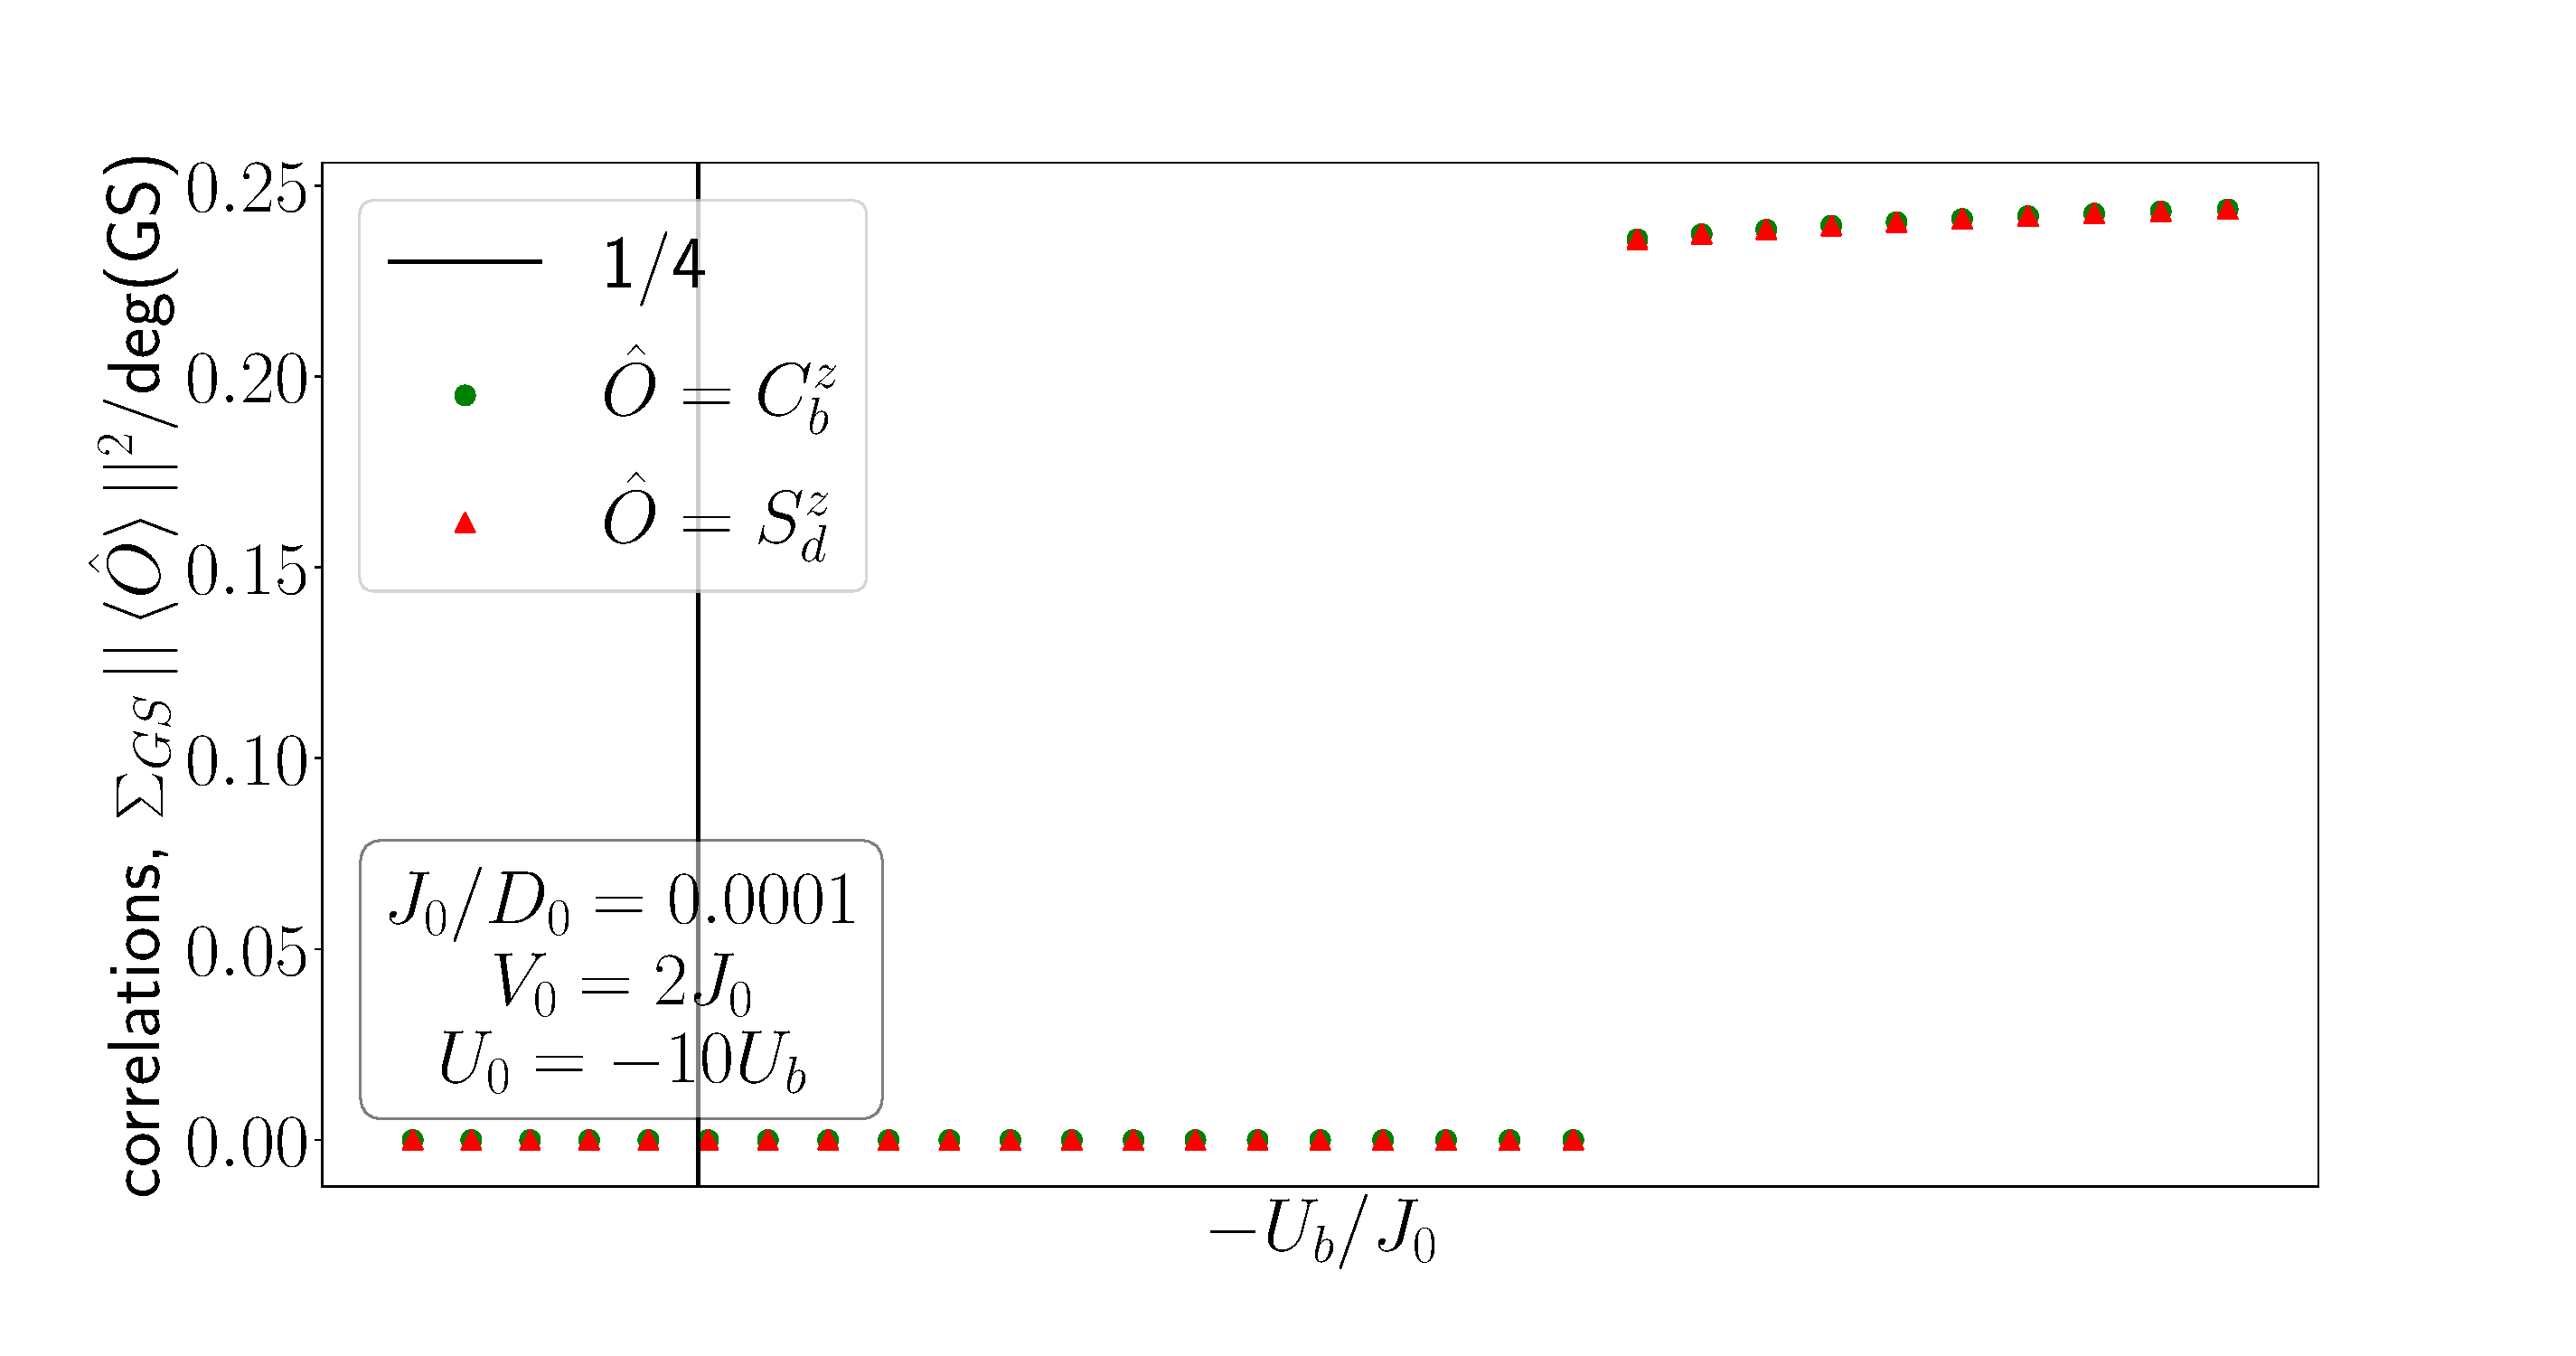
\includegraphics[width=\textwidth]{./figures/corrs_gs-J=0.100.pdf}
}

\only<2>{\(J_0/D_0 = 10^{-2}\)

\vspace*{-20pt}
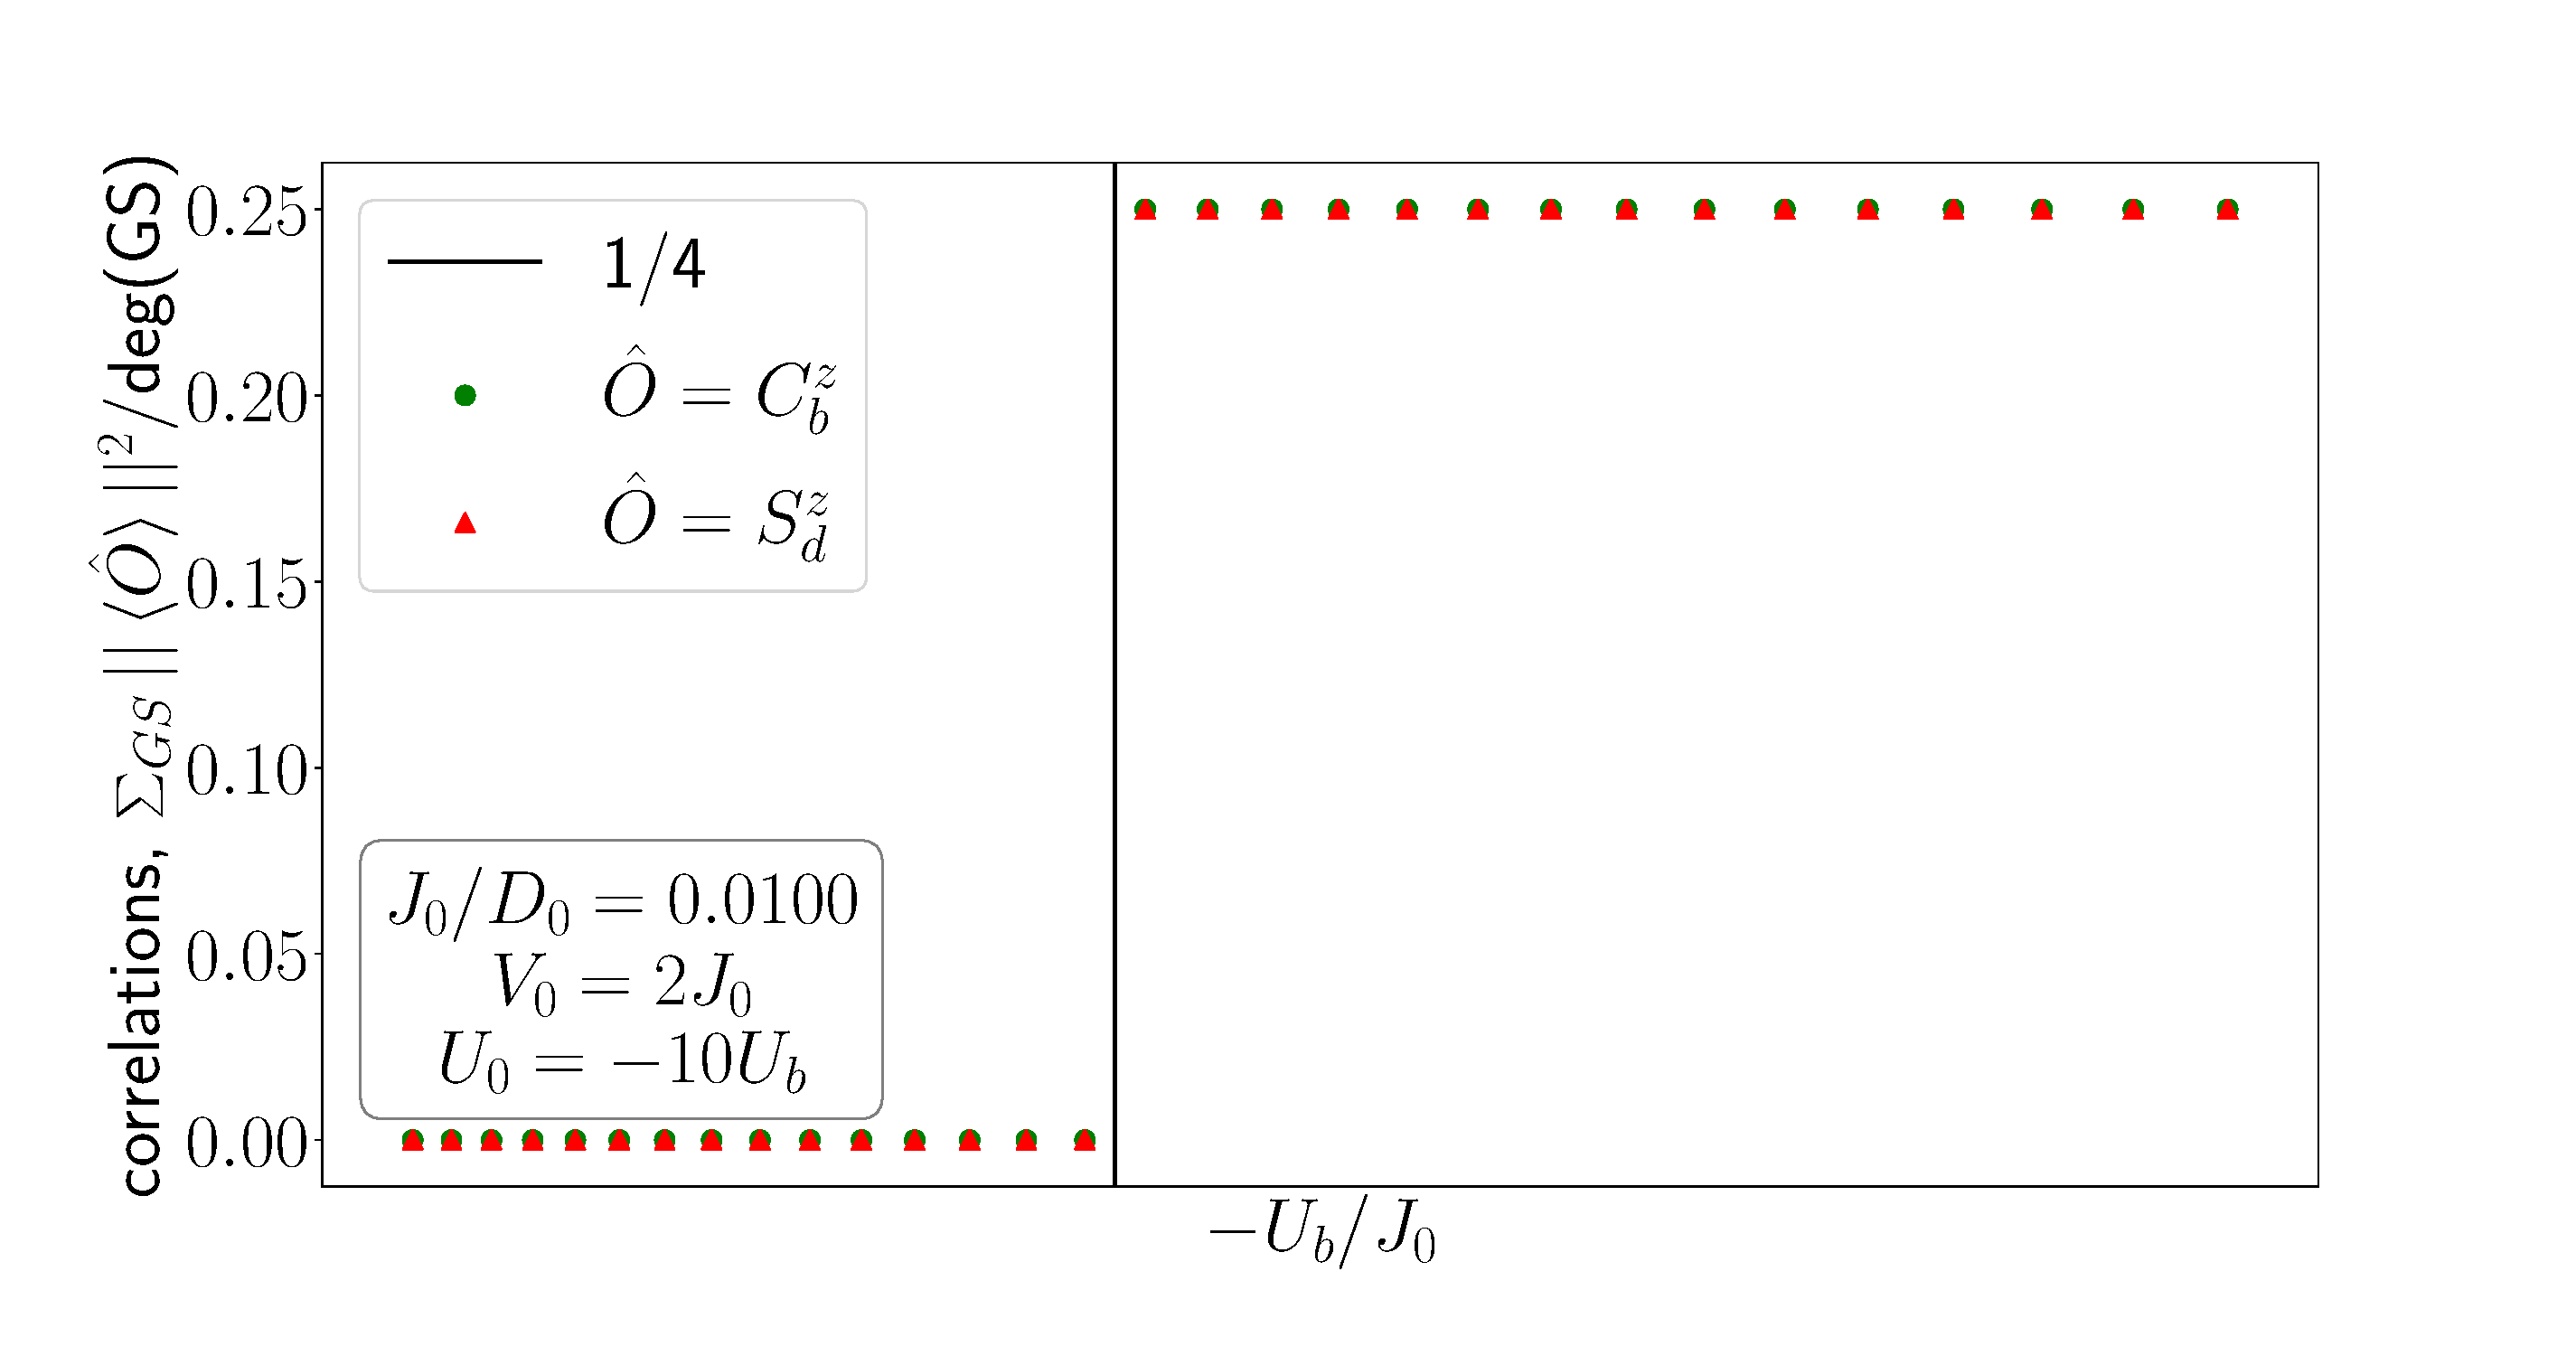
\includegraphics[width=\textwidth]{./figures/corrs_gs-J=10.000.pdf}}

\only<3>{\(J_0/D_0 = 10^{-1}\)

\vspace*{-20pt}
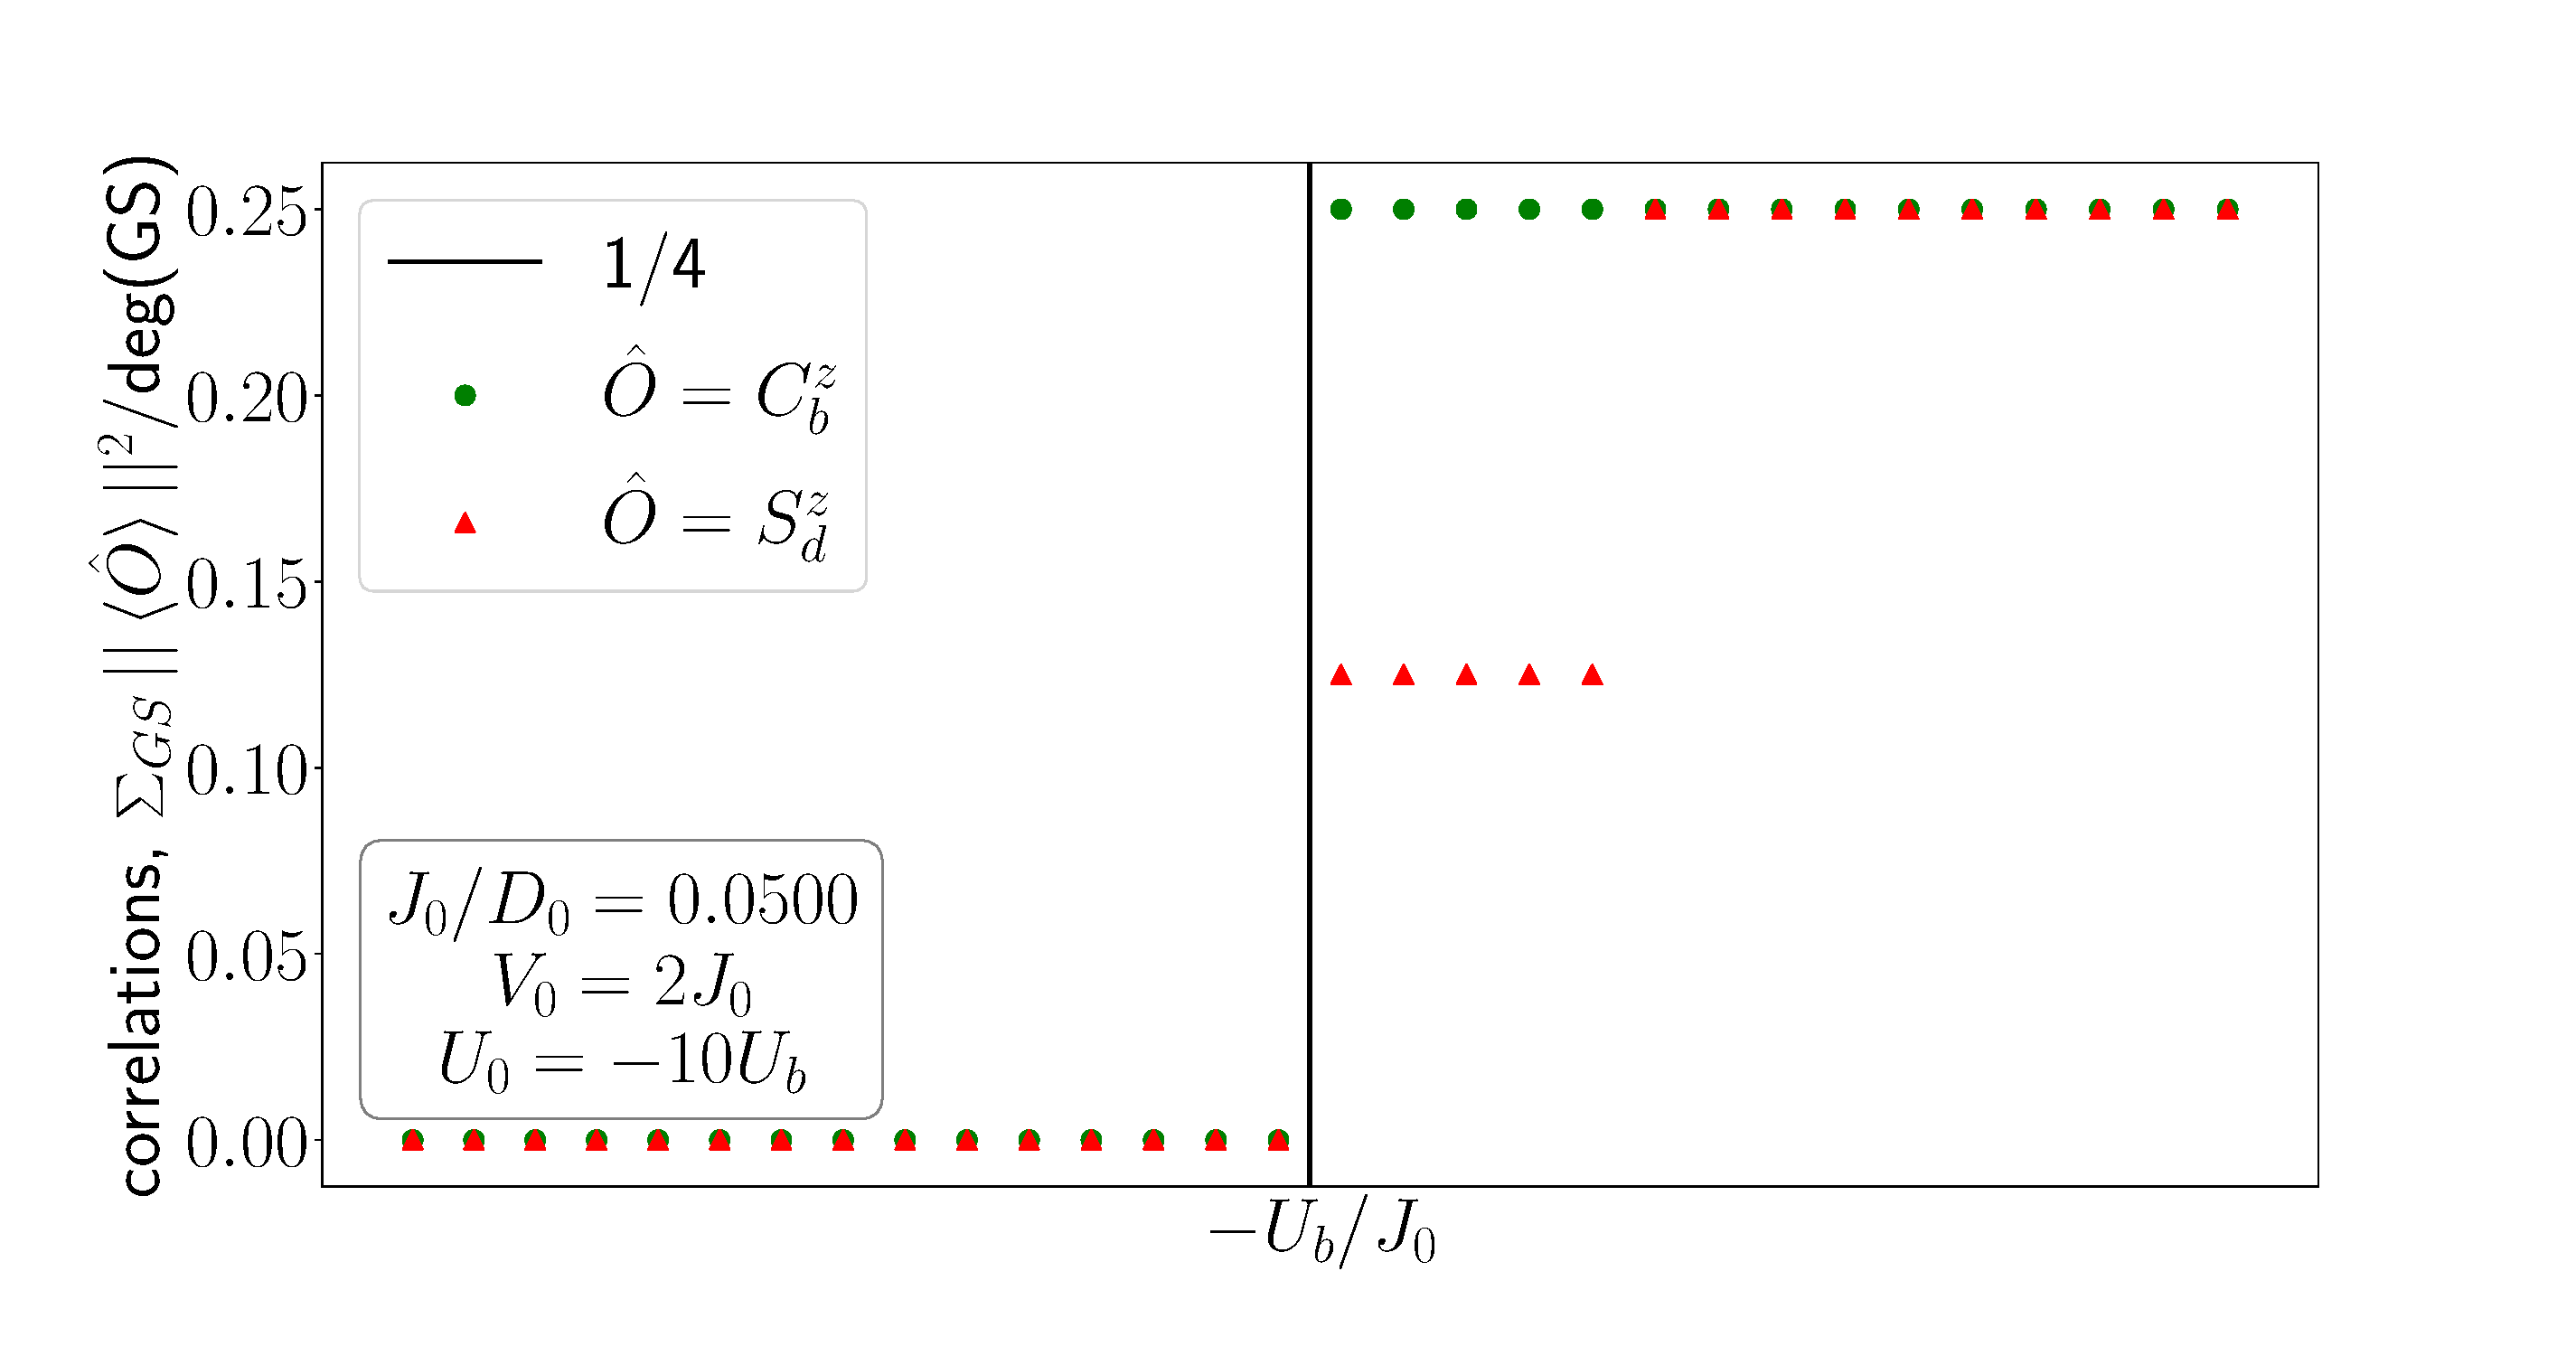
\includegraphics[width=\textwidth]{./figures/corrs_gs-J=50.000.pdf}}

\end{frame}

\begin{frame}[noframenumbering]{Correlation measures}
\only<+>{
\head{Local Fermi liquid}
\vspace*{20pt}
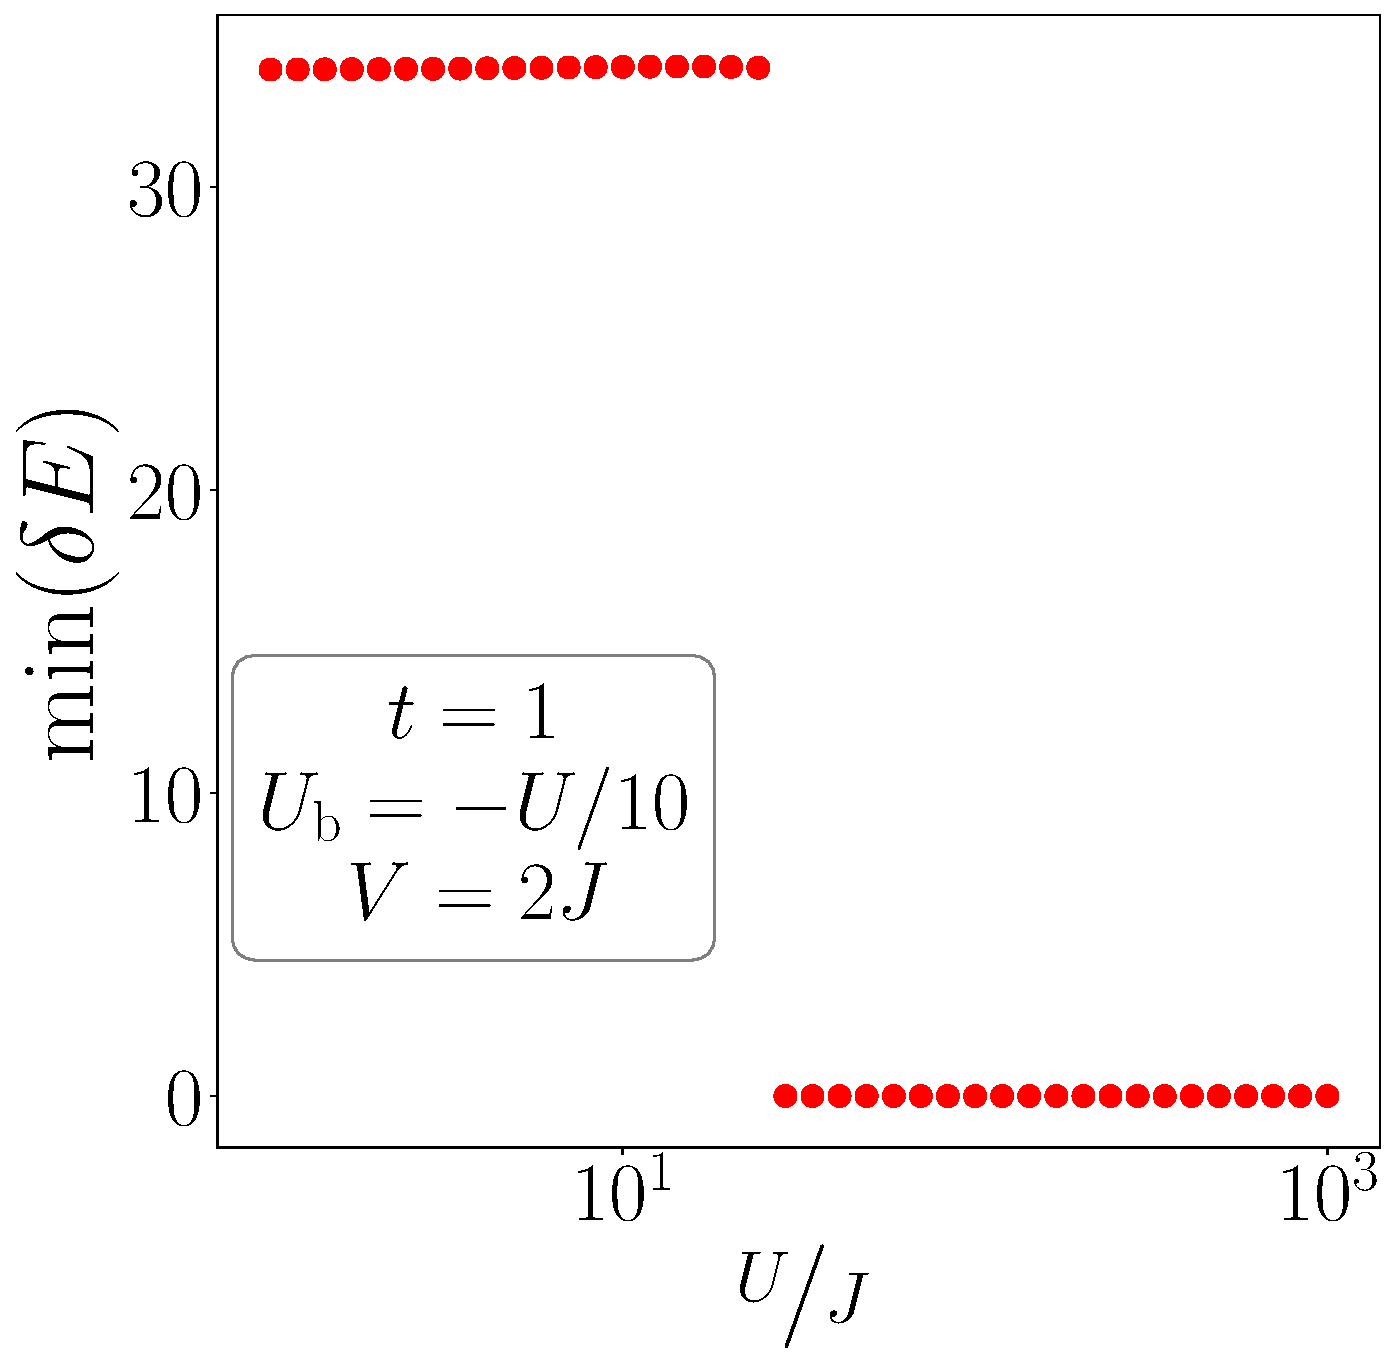
\includegraphics[width=0.49\textwidth]{./figures/gap-t=1.000,J=10.000,0.000,40,V=3J,Ubath=-U_by_10,N=4,U=1.000,1000.000,40.pdf}
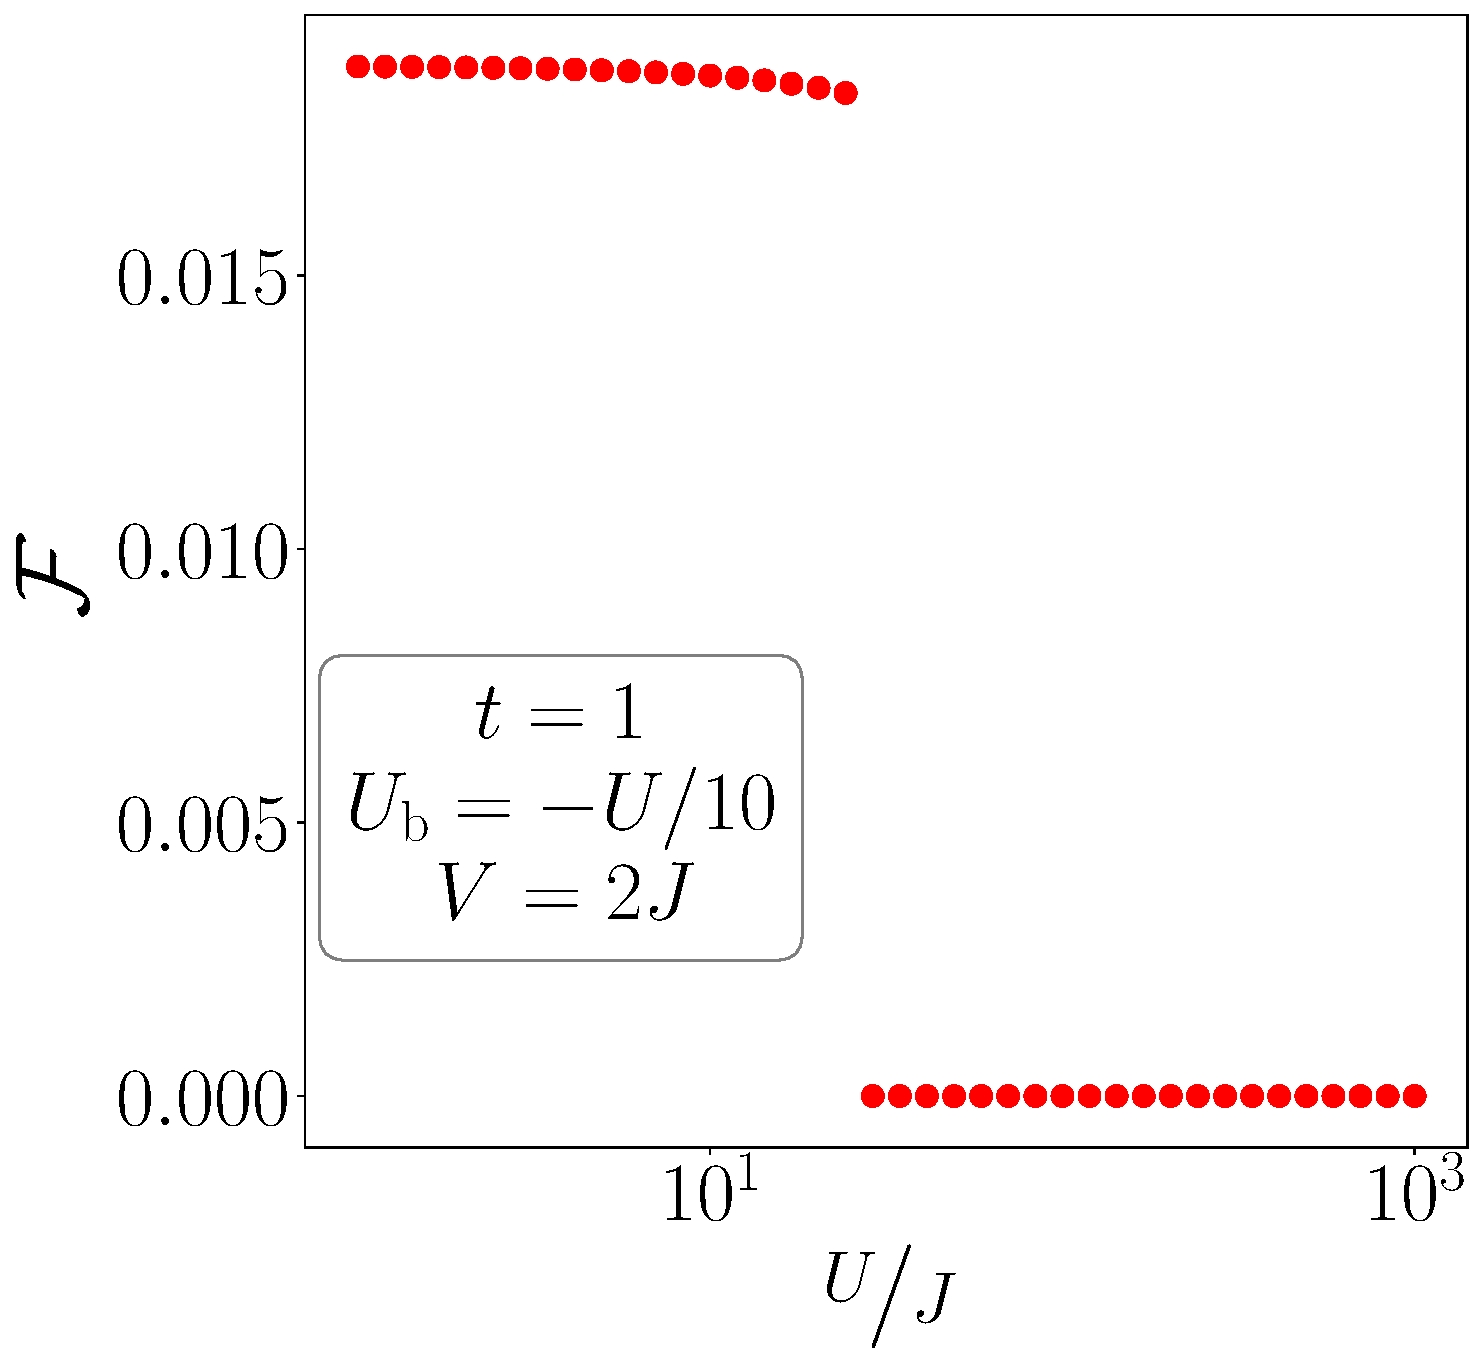
\includegraphics[width=0.49\textwidth]{./figures/lfl-t=1.000,J=10.000,0.000,40,V=3J,Ubath=-U_by_10,N=4,U=1.000,1000.000,40.pdf}
}
\only<+>{
\head{Kondo cloud}
\vspace*{20pt}
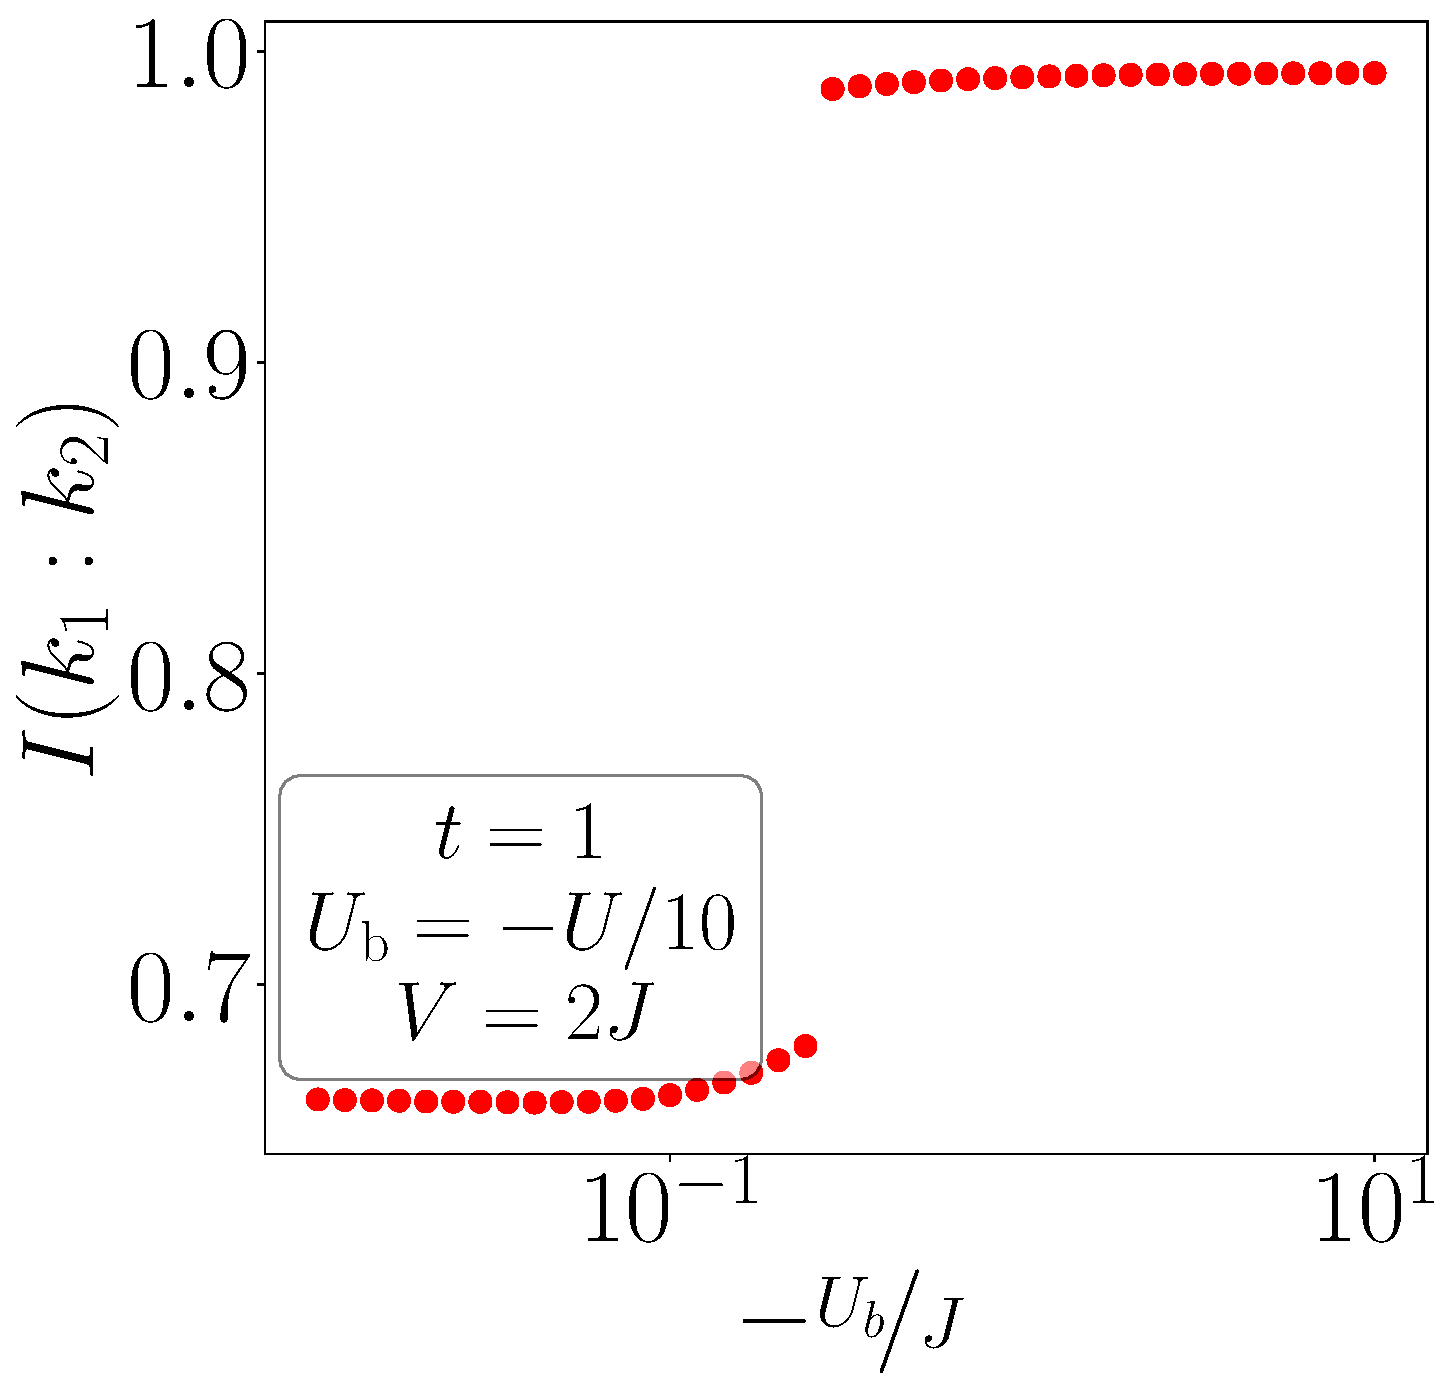
\includegraphics[width=0.49\textwidth]{./figures/corr-k-t=1.000,J=10.000,0.000,40,V=3J,Ubath=-U_by_10,N=4,U=1.000,1000.000,40.pdf}
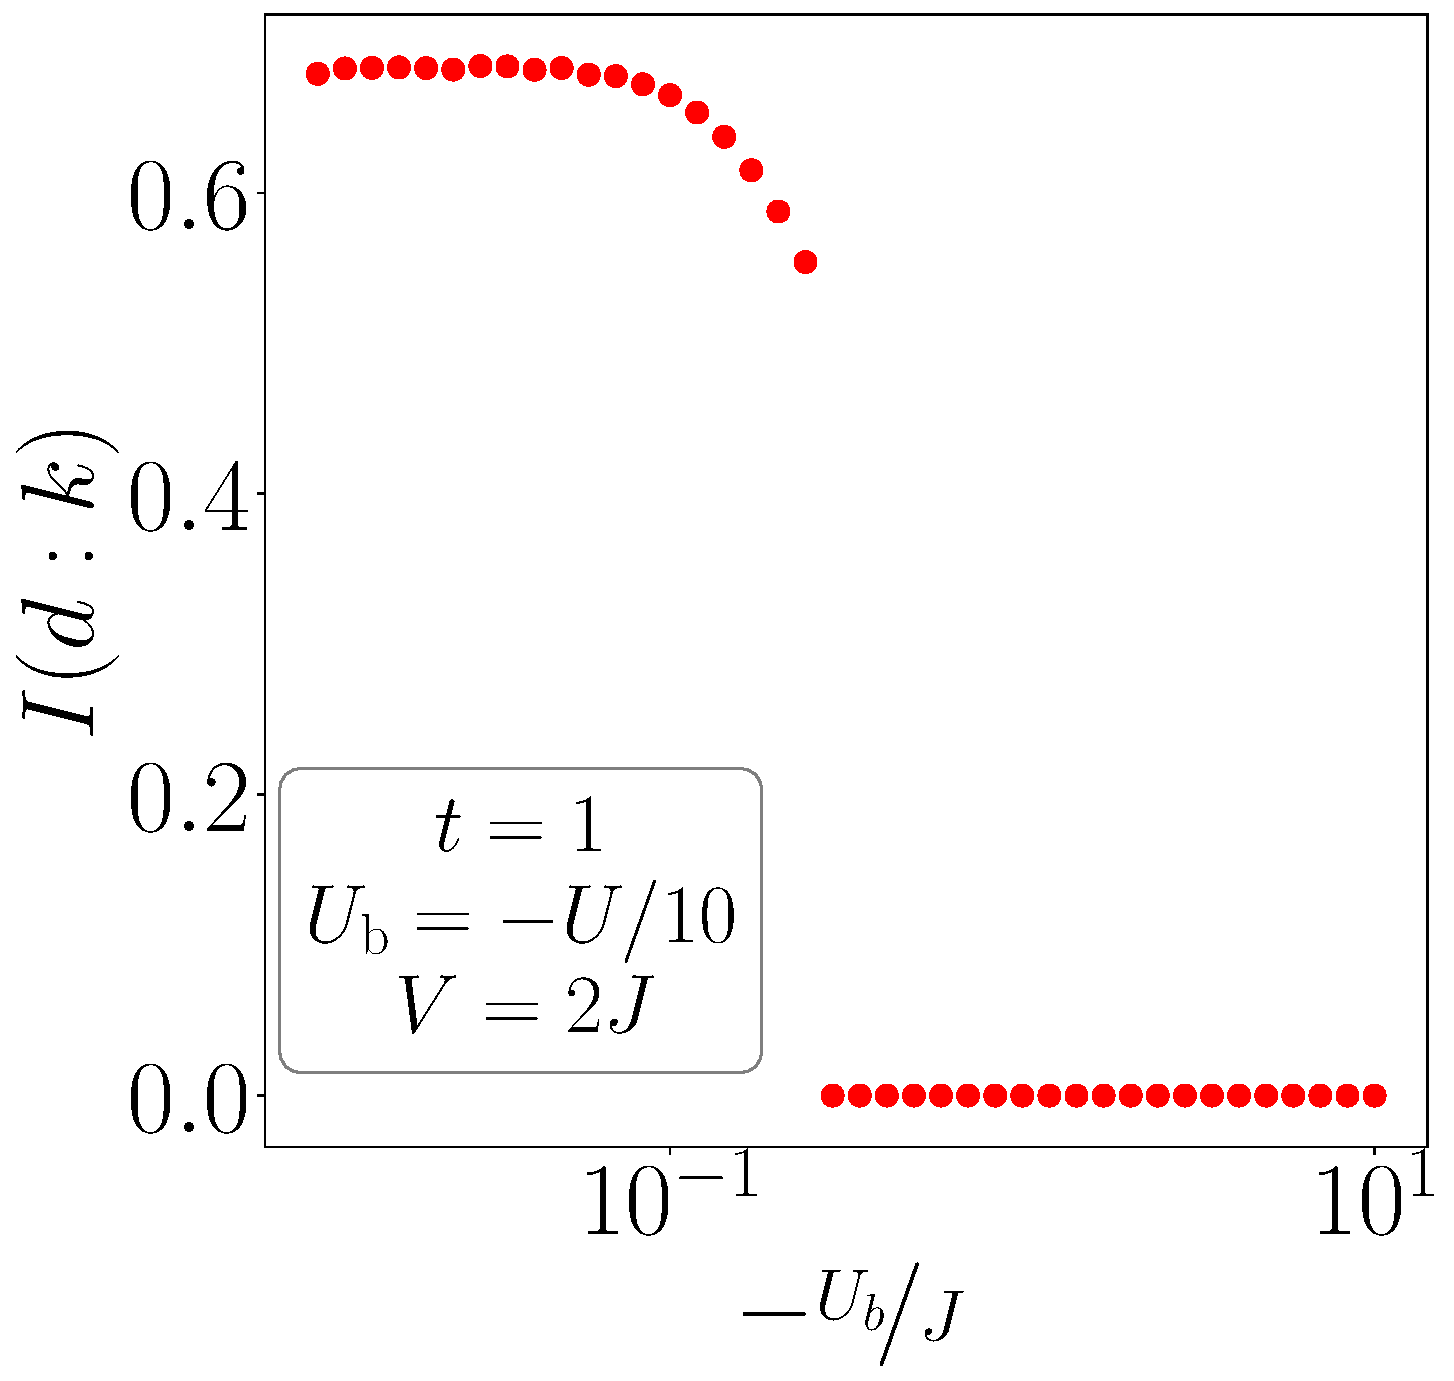
\includegraphics[width=0.49\textwidth]{./figures/mi-dk-t=1.000,J=10.000,0.000,40,V=3J,Ubath=-U_by_10,N=4,U=1.000,1000.000,40.pdf}
}
\only<+>{
\head{Real space mutual information}
\vspace*{20pt}
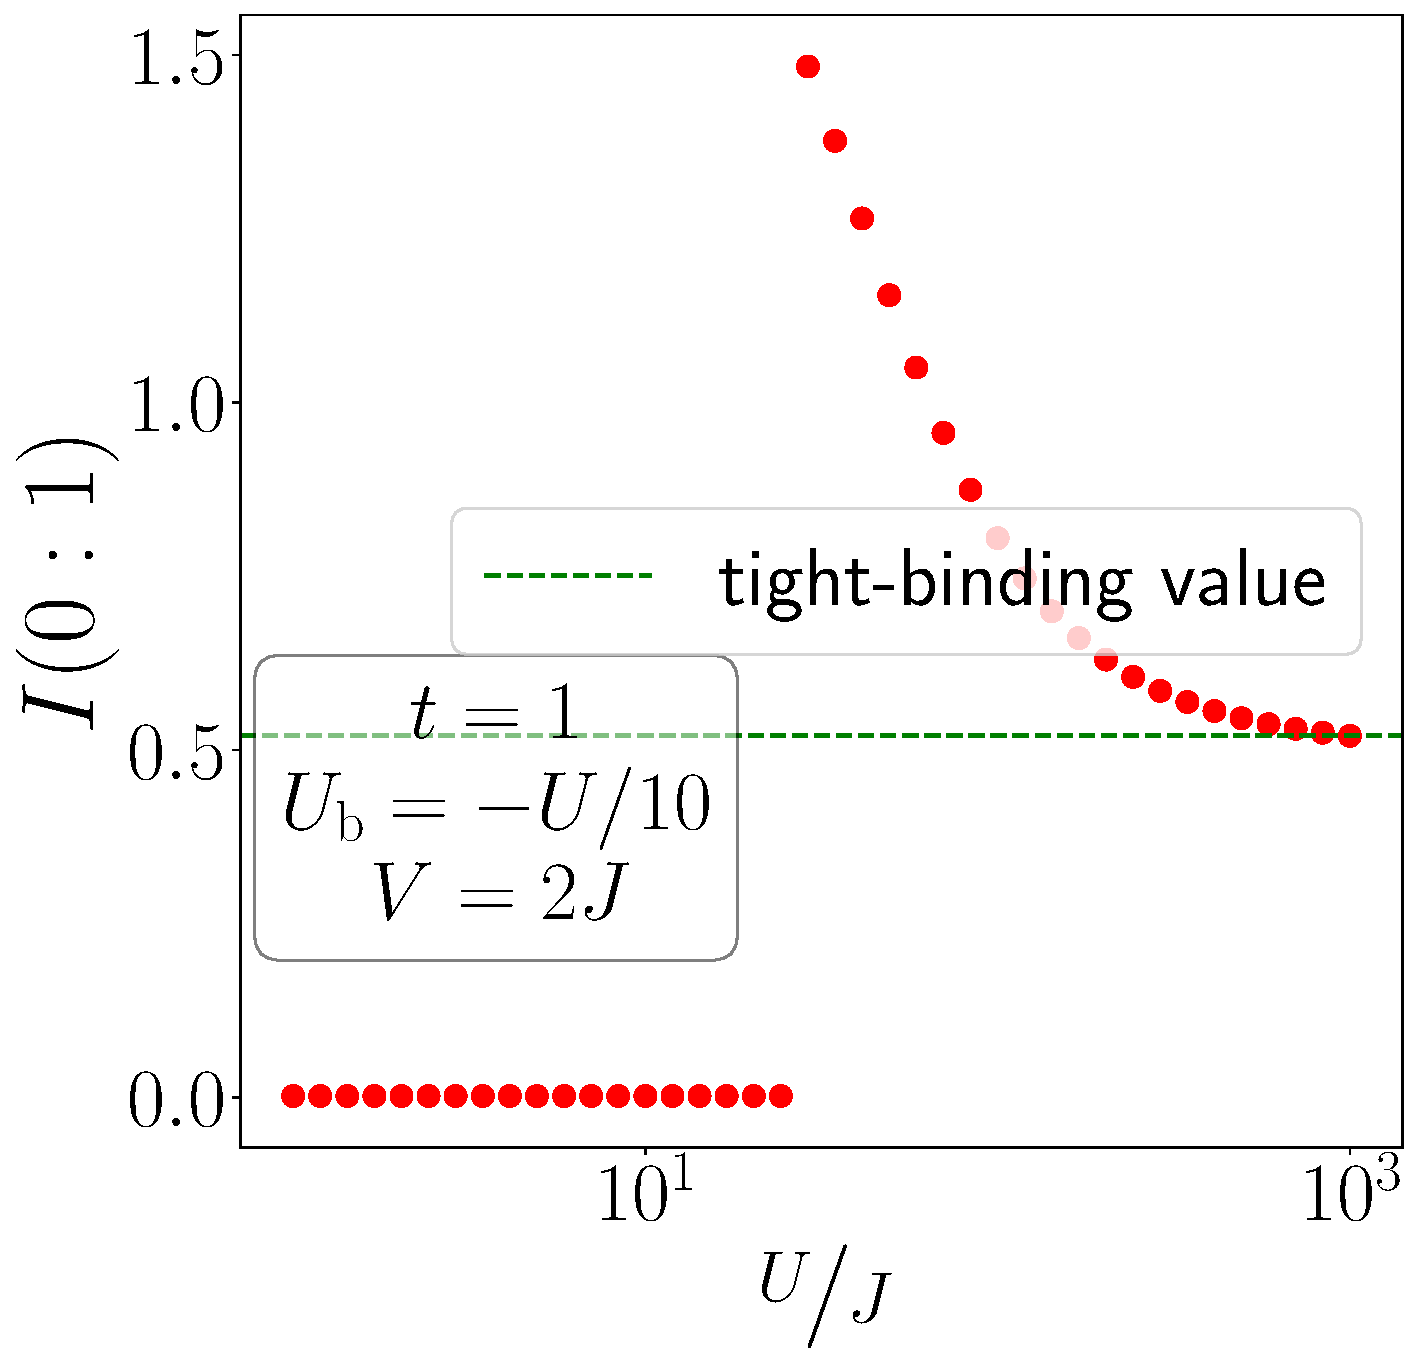
\includegraphics[width=0.49\textwidth]{./figures/mi-01-t=1.000,J=10.000,0.000,40,V=3J,Ubath=-U_by_10,N=4,U=1.000,1000.000,40.pdf}
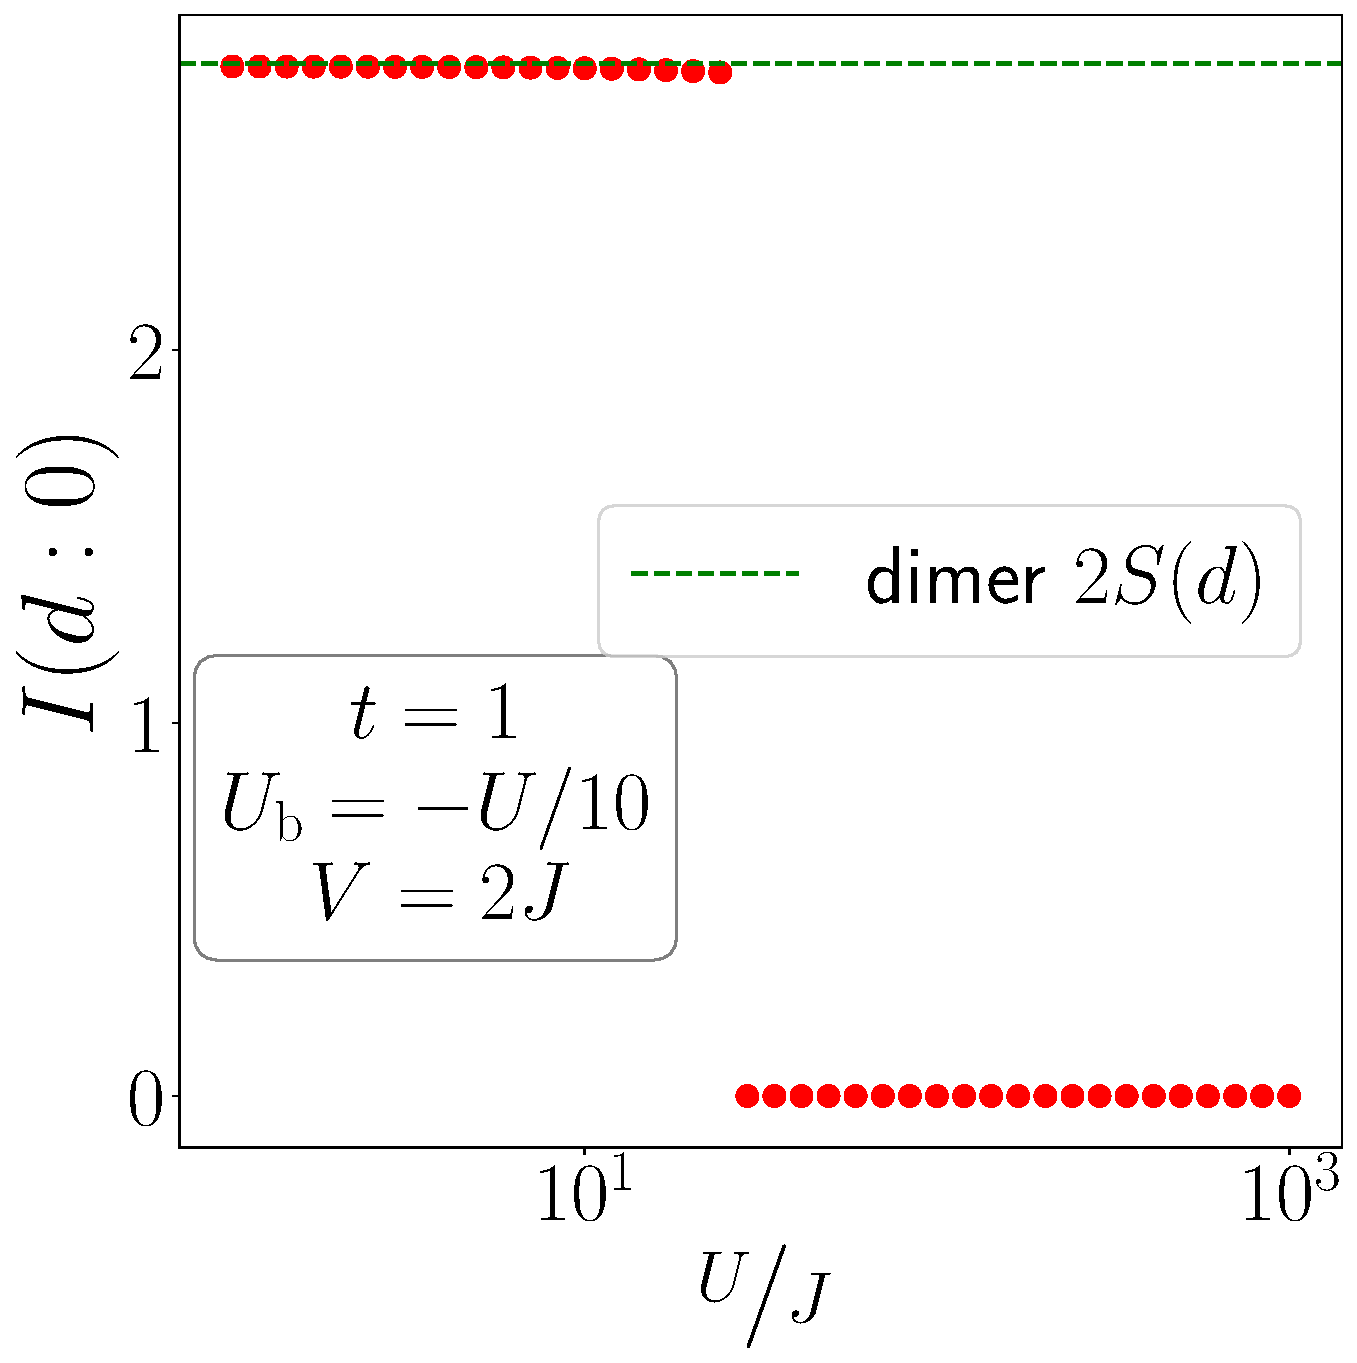
\includegraphics[width=0.49\textwidth]{./figures/mi-d0-t=1.000,J=10.000,0.000,40,V=3J,Ubath=-U_by_10,N=4,U=1.000,1000.000,40.pdf}
}

\only<+>{
\head{Impurity entanglement entropy and spin-spin correlations}
\vspace*{20pt}
	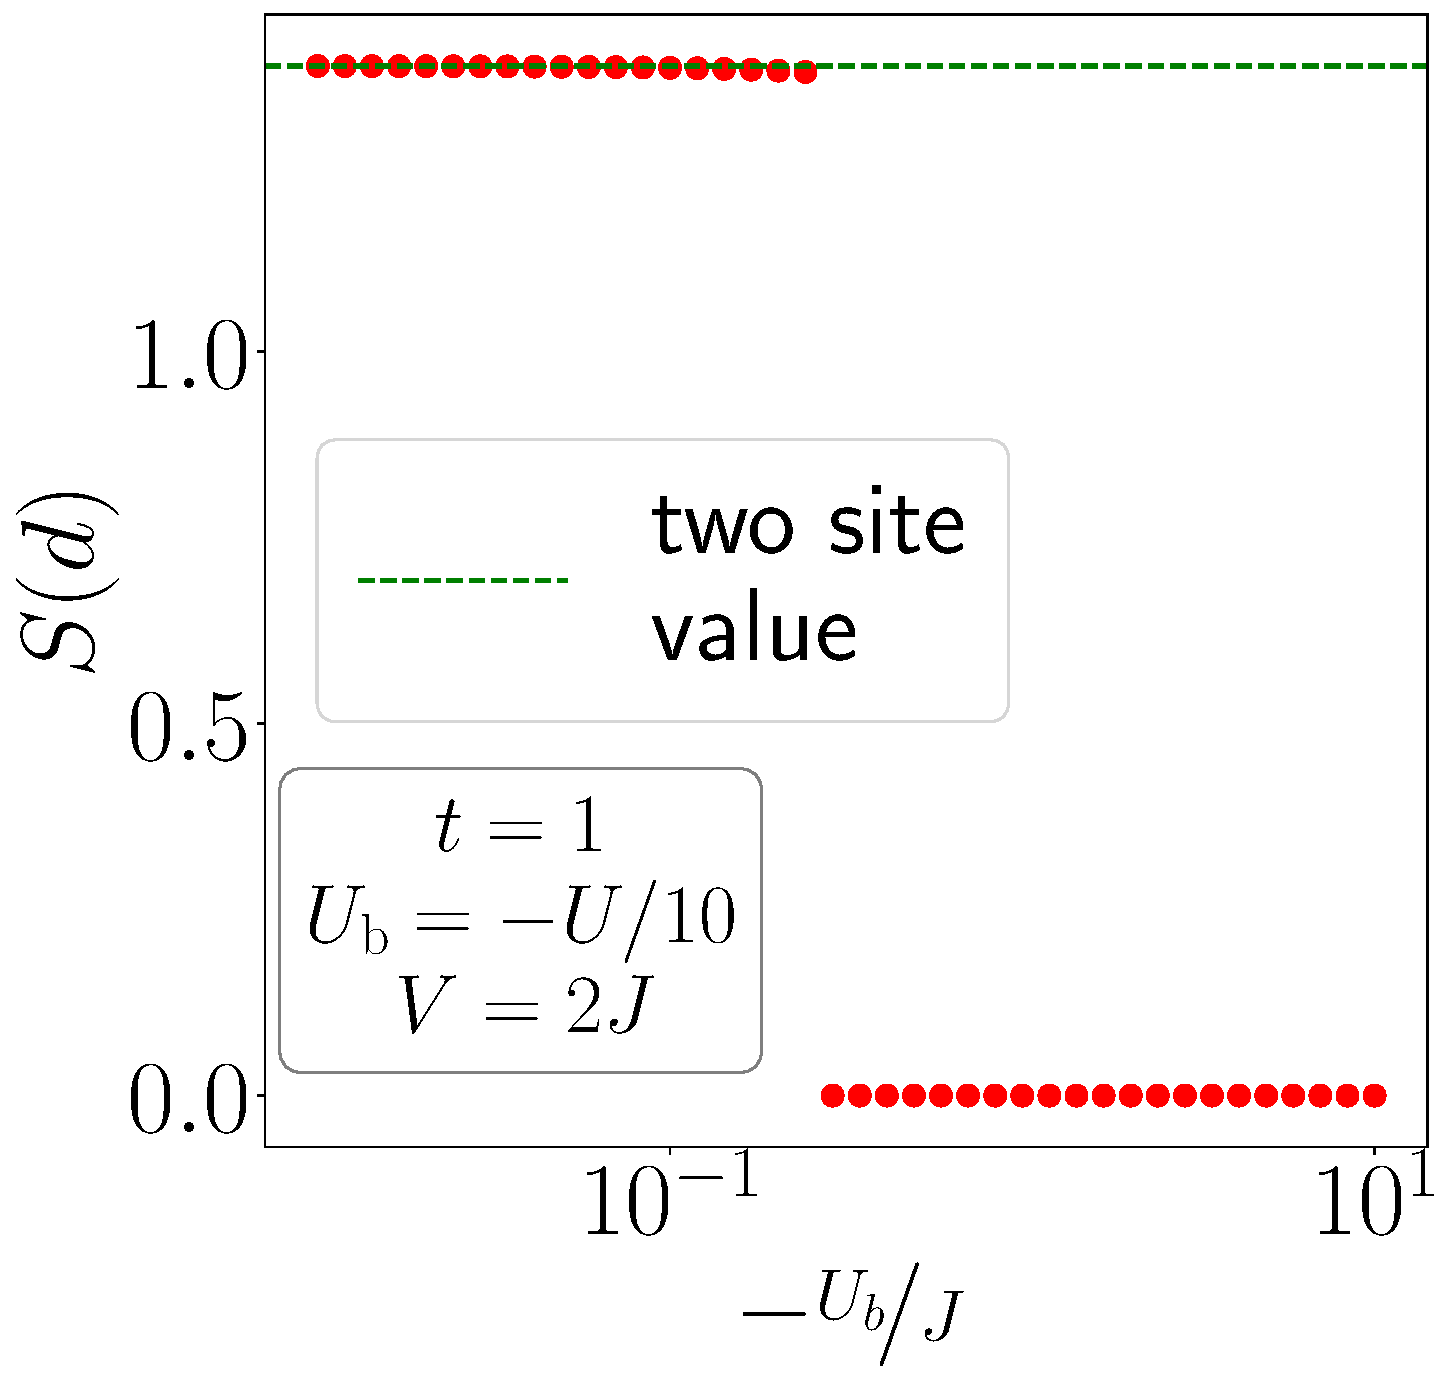
\includegraphics[width=0.32\textwidth]{./figures/EE-d-t=1.000,J=10.000,0.000,40,V=3J,Ubath=-U_by_10,N=4,U=1.000,1000.000,40.pdf}
	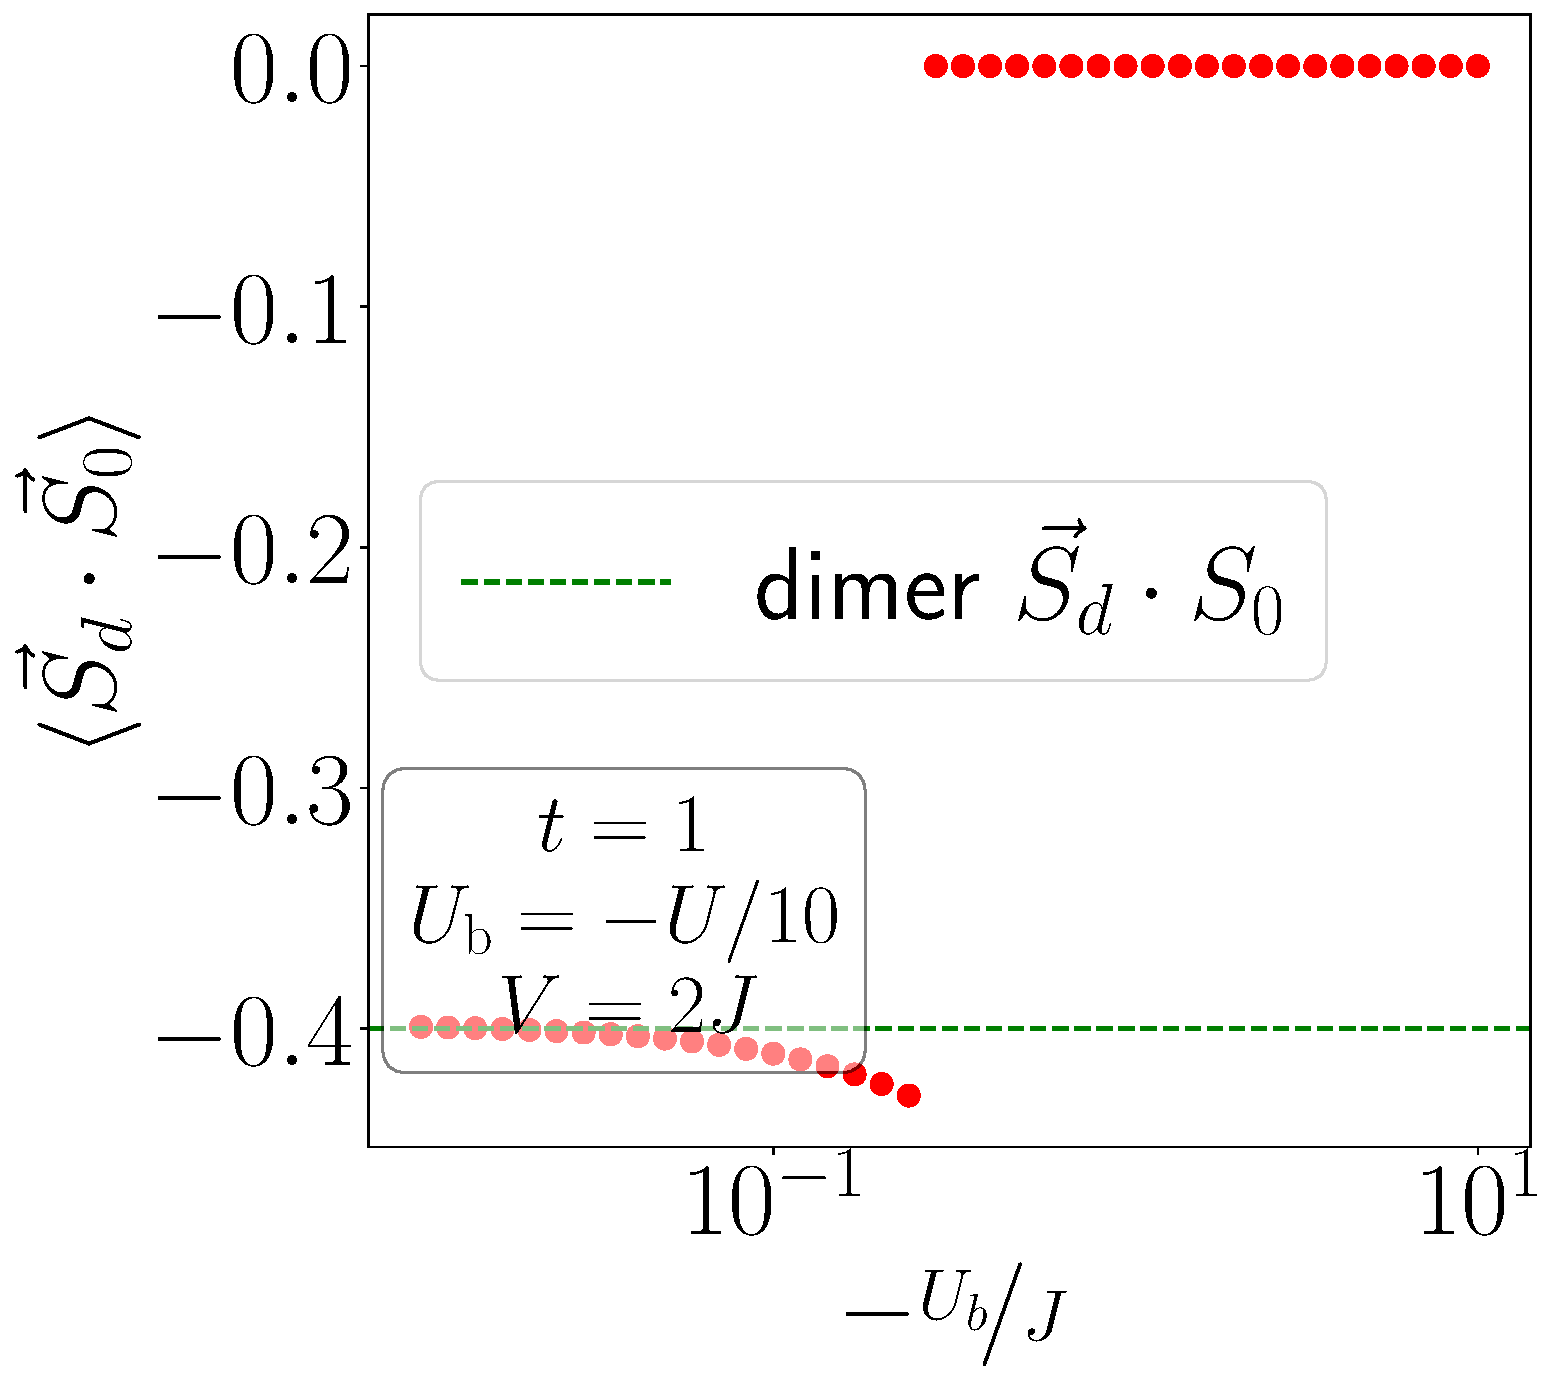
\includegraphics[width=0.32\textwidth]{./figures/corr-d0-t=1.000,J=10.000,0.000,40,V=3J,Ubath=-U_by_10,N=4,U=1.000,1000.000,40.pdf}
	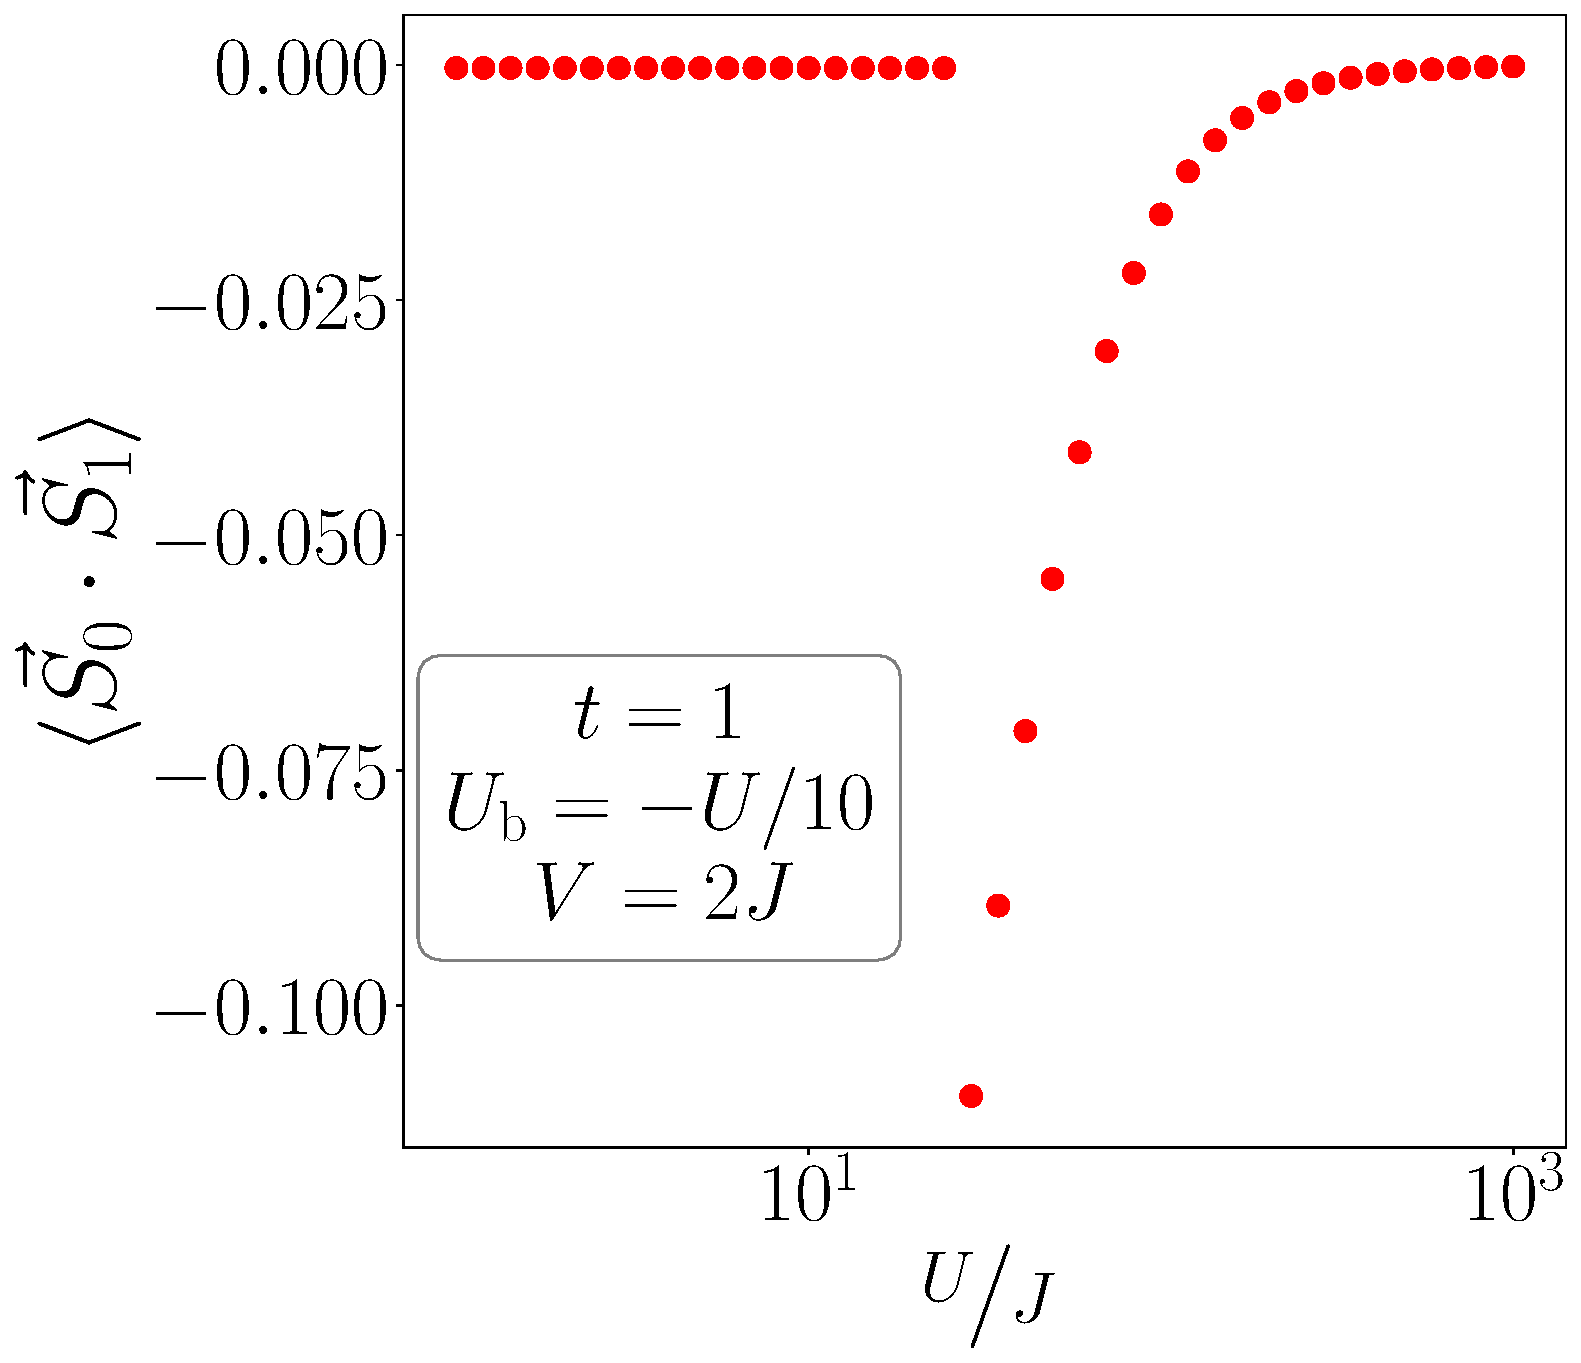
\includegraphics[width=0.32\textwidth]{./figures/r-vec-corr-01-t=1.000,J=10.000,0.000,40,V=3J,Ubath=-U_by_10,N=4,U=1.000,1000.000,40.pdf}
}

\only<+>{
\head{Real-space correlations}
\vspace*{20pt}
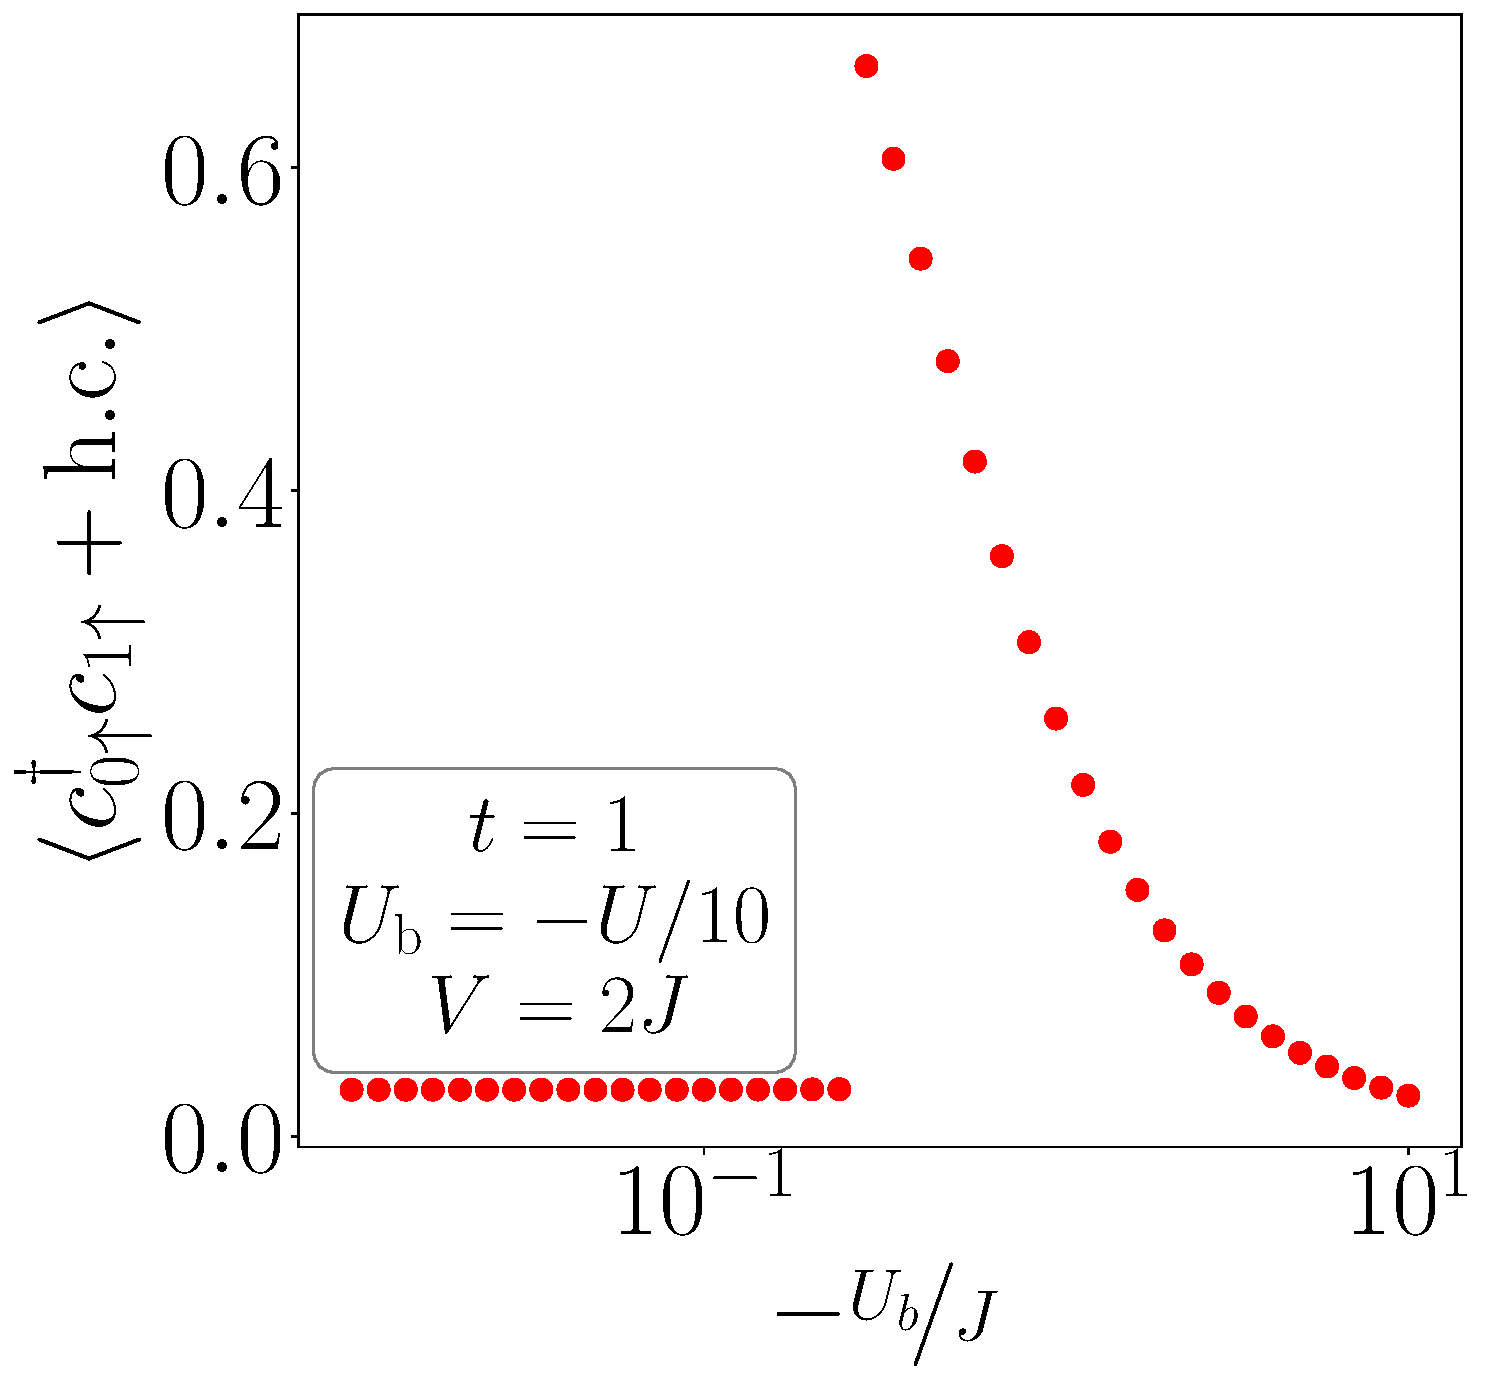
\includegraphics[width=0.49\textwidth]{./figures/r1p-t=1.000,J=10.000,0.000,40,V=3J,Ubath=-U_by_10,N=4,U=1.000,1000.000,40.pdf}
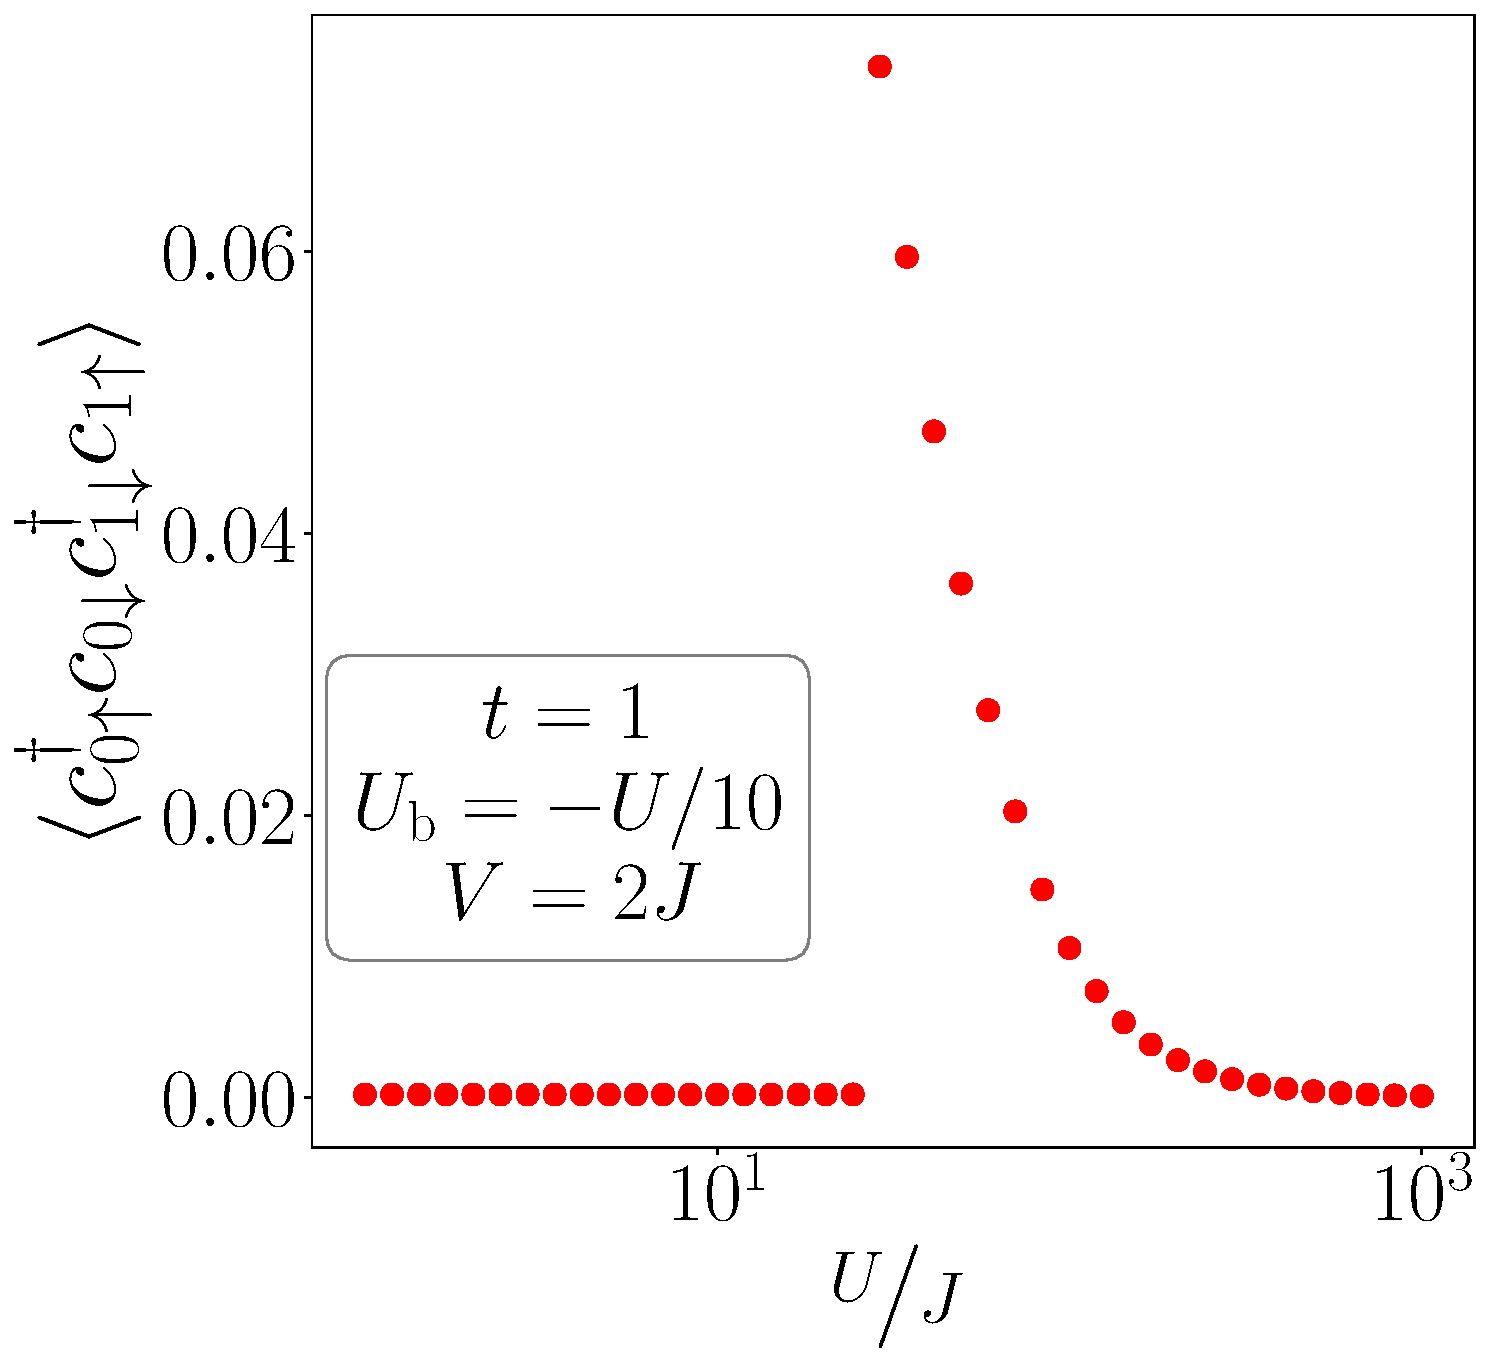
\includegraphics[width=0.49\textwidth]{./figures/r-od-t=1.000,J=10.000,0.000,40,V=3J,Ubath=-U_by_10,N=4,U=1.000,1000.000,40.pdf}
}

\end{frame}

\section{Zero-bandwidth limit of fixed point Hamiltonian}
\begin{frame}[noframenumbering]{Zero-bandwidth limit of fixed point Hamiltonian}
\only<1>{
	\head{Route to the zero-bandwidth model}
	At strong-coupling fixed point,
	\begin{itemize}
	\item kinetic energy acts as a perturbation
	\item \focus{compress the bandwidth to just the Fermi surface}

		\[H^*_\text{zero bw} = \left(\epsilon_F - \mu\right) \hat n_{k_F} + \frac{U^*}{2}\left( \hat n_{d \uparrow} - \hat n_{d \downarrow} \right)^2 + V^*\sum_\sigma \left(c^\dagger_{d\sigma}c_{0\sigma} + \text{h.c.}\right)  + J \vec{S}_d\cdot\vec{s}_0\]
		\[\focus{\text{(center of motion)}}\]\\[10pt]

	\item Setting \(\mu = \epsilon_F\) gives a \focus{two-site model}

	\[H^*_\text{zero} = \frac{U^*}{2}\left( \hat n_{d \uparrow} - \hat n_{d \downarrow} \right)^2 + V^*\sum_\sigma \left(c^\dagger_{d\sigma}c_{0\sigma} + \text{h.c.}\right)  + J \vec{S}_d\cdot\vec{s}_0\]
	\end{itemize}
}
\only<2>{
	\head{Effective two-site problem}
	\centering

	\[H^*_\text{zero} = J^* \vec{S}_d\cdot\vec{s}_< + H^*_\text{IOMS}\]

	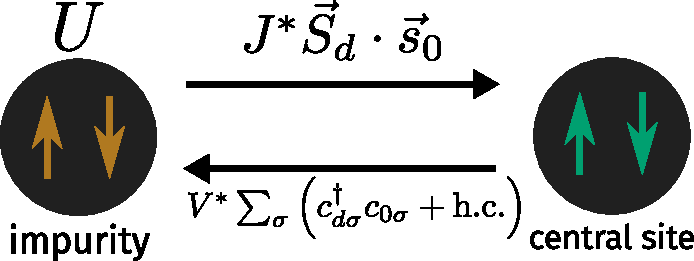
\includegraphics[width=0.6\textwidth]{figures/kondo_zeromode.pdf}

	\[\ket{\Psi}_\text{gs} = \frac{c_s}{\sqrt 2}\left(\ket{\uparrow,\downarrow} - \ket{\downarrow, \uparrow}\right) + \frac{\sqrt{1 - c_s^2}}{\sqrt 2}\left(\ket{2,0} + \ket{0,2}\right), ~ ~ c_s \to 1 \text{ as } D \to \infty\]
}

\end{frame}

\section{Local Fermi liquid excitations}
\begin{frame}[noframenumbering]{Local Fermi liquid excitations}
\head{Effective Hamiltonian in singlet subspace}
\only<1>{We treat the dispersion as a \focus{real-space nearest neighbour hopping}.
\vspace{20pt}

}
\begin{minipage}{0.5\textwidth}
\only<1>{
\[H^* = -\frac{U}{2}\left(\hat n_{d \uparrow} - \hat n_{d \downarrow}\right)^2 + J^* \vec{S}_d\cdot\vec{s}_0\]
\[ + V\sum_\sigma \left(c^\dagger_{d\sigma}c_{0\sigma} + \text{h.c.}\right) \]
\[\color{maroon}{- t\sum_{i\sigma}\left(c^\dagger_{i\sigma}c_{i+1,\sigma} + \text{h.c.}\right)}\]
}
\only<2>{Initially consider \focus{just the first site}. Treat \focus{hopping as perturbation}:
\[\ket{\Psi}^*_{GS} = c_s\ket{SS} + \sqrt{1 - c_s^2}\ket{CT,0}\]
\[ V =- t\sum_{\sigma}\left(c^\dagger_{0\sigma}c_{1,\sigma} + \text{h.c.}\right)\]
}
\only<3>{Upto \focus{fourth order}, effective Hamiltonian is
	\[H^*_\text{eff} = \text{constant} + \alpha \mathcal{P}_\text{charge}\]
\[\mathcal{P}_\text{charge} \longrightarrow \text{projector onto }\hat n_1 \neq 1\]
\begin{itemize}
	\item For \(U \ll V \ll J\), we get \(0 < \alpha \ll 1\)
	\item a \focus{very weak local FL} on $1^\text{st}$ site
\end{itemize}
}
\end{minipage}
\begin{minipage}{0.4\textwidth}
	\only<1>{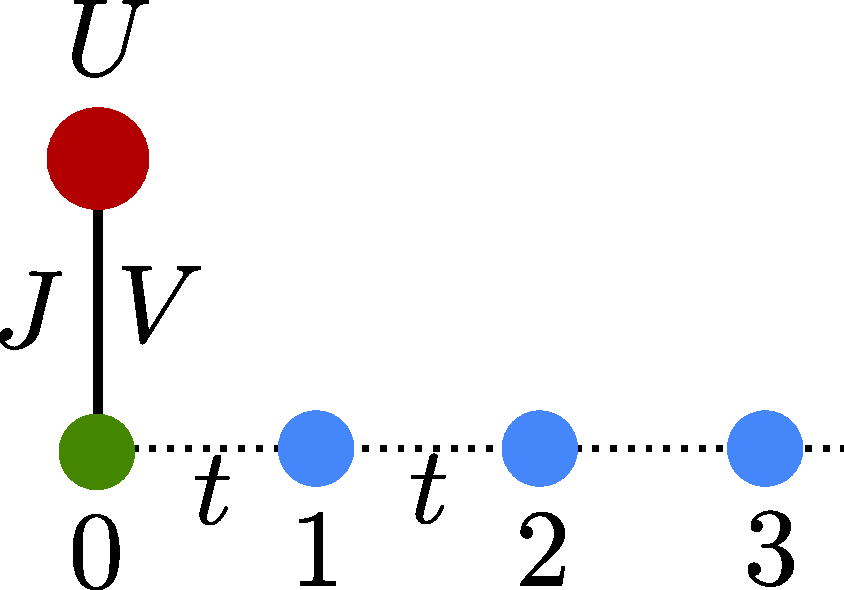
\includegraphics[width=0.9\textwidth]{figures/noz_1D.pdf}}
	\only<2>{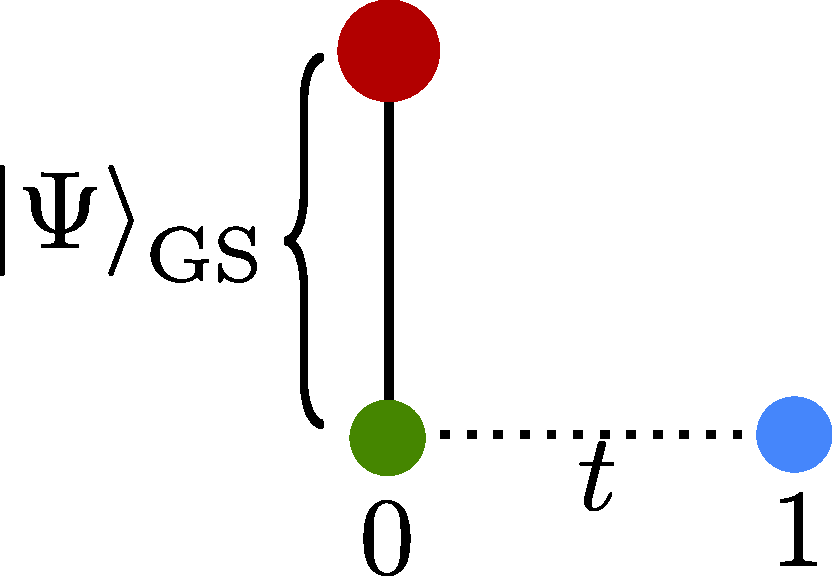
\includegraphics[width=0.9\textwidth]{figures/noz_1D_approx.pdf}}
	\only<3>{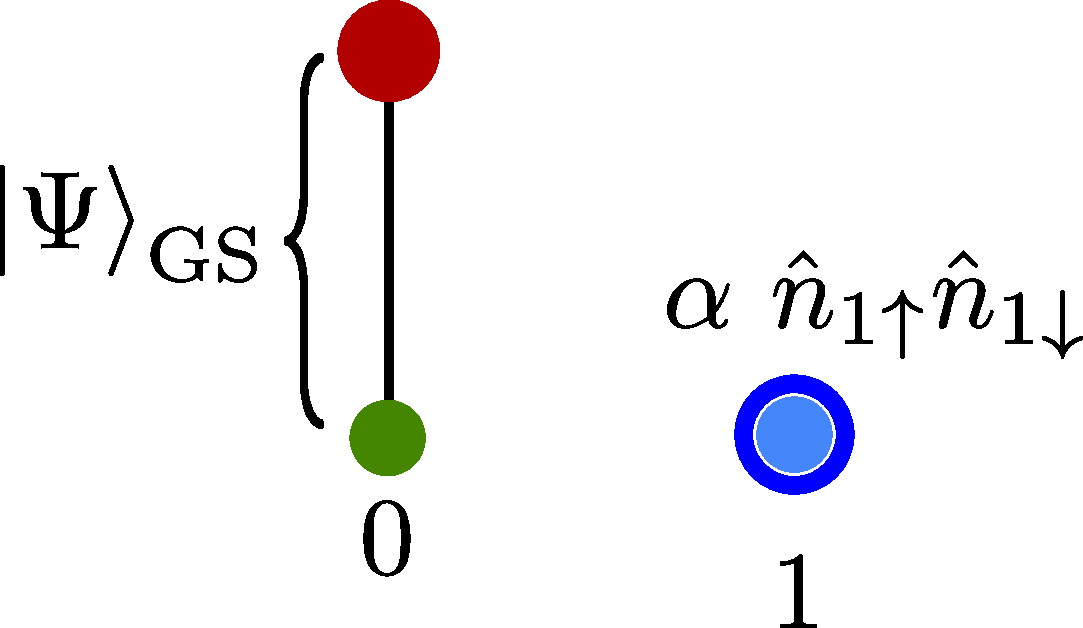
\includegraphics[width=0.9\textwidth]{figures/lattice_eff.pdf}}
\end{minipage}
\end{frame}

\section{Signatures of breakdown of screening - Journey towards local moment phase}

\centering
\begin{frame}[noframenumbering]{}
\begin{itemize}
	\item We will work with a Hilbert space of (6+1=)~\focus{7 sites}
	\item \focus{Recreate RG flow} by tuning the parameters \(U,V,J\)
	\item \focus{Observe various measures} of entanglement and correlation along this variation
\end{itemize}

\vspace*{20pt}
\hspace{\fill}
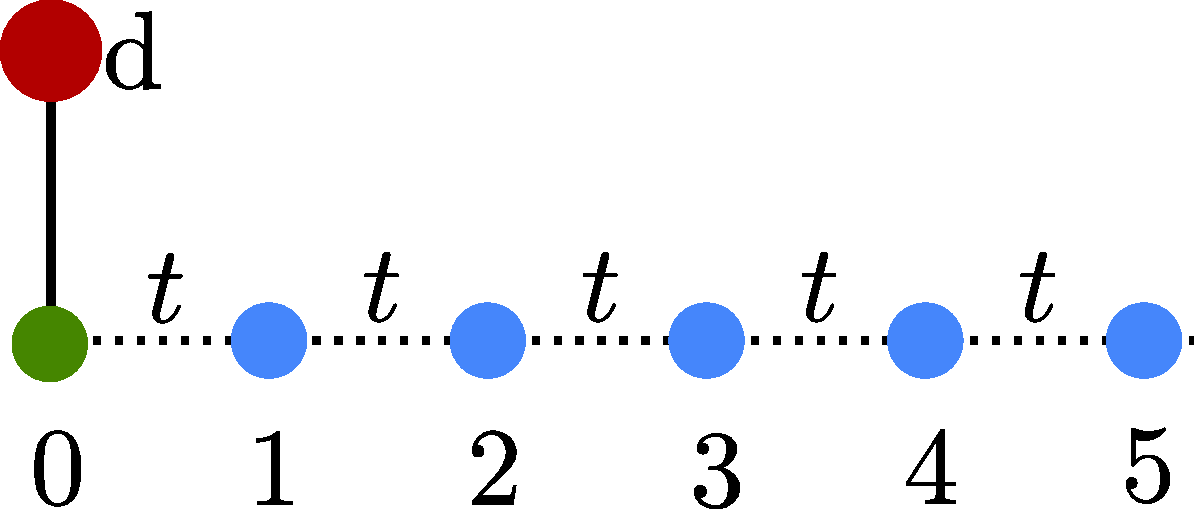
\includegraphics[width=0.45\textwidth]{figures/seven_site.pdf}
\hspace{\fill}
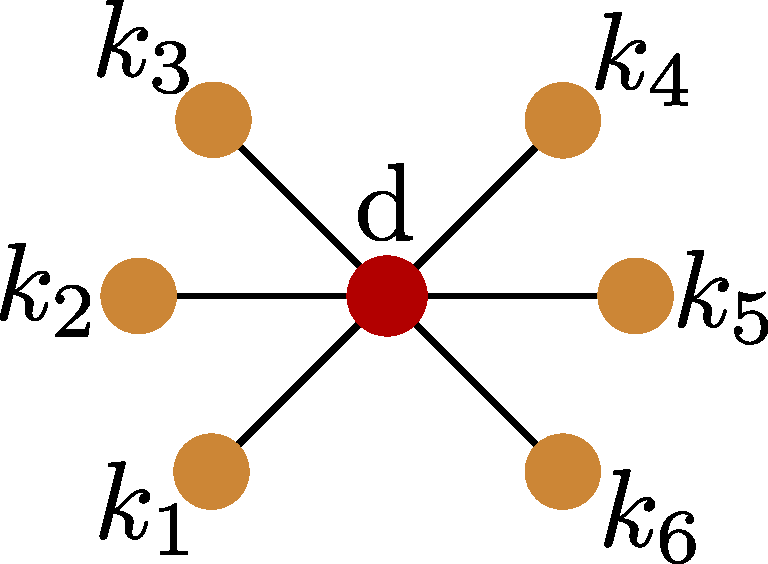
\includegraphics[width=0.3\textwidth]{figures/seven_site2.pdf}
\hspace{\fill}
\end{frame}

% \begin{frame}[noframenumbering]{Breakdown of renormalised perturbation theory}

% \head{Perturbation parameter, zero mode gap and local FL strength}

% \vspace*{25pt}
% {
% \centering
% 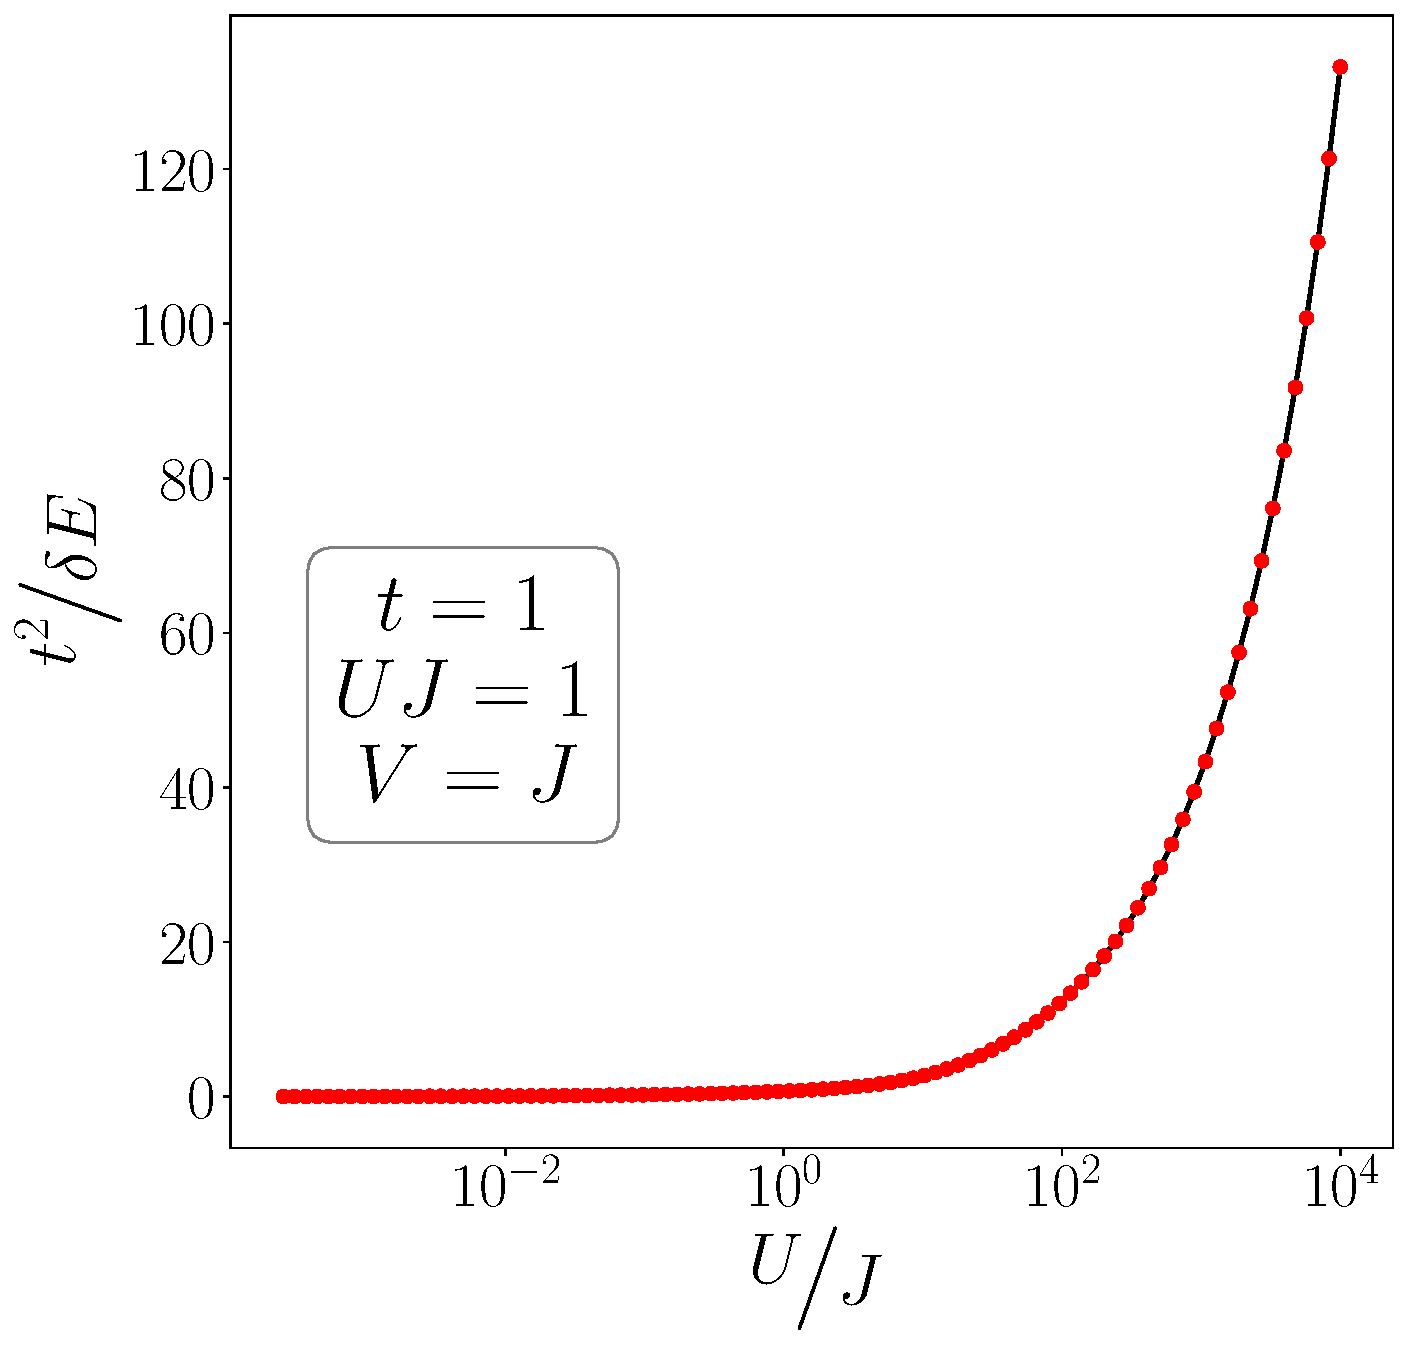
\includegraphics[width=0.3\textwidth]{figures/par-t=1.000,J=1_over_U,V=J,N=4,U=0.016,100.000,95.pdf}
% \hspace*{\fill}
% 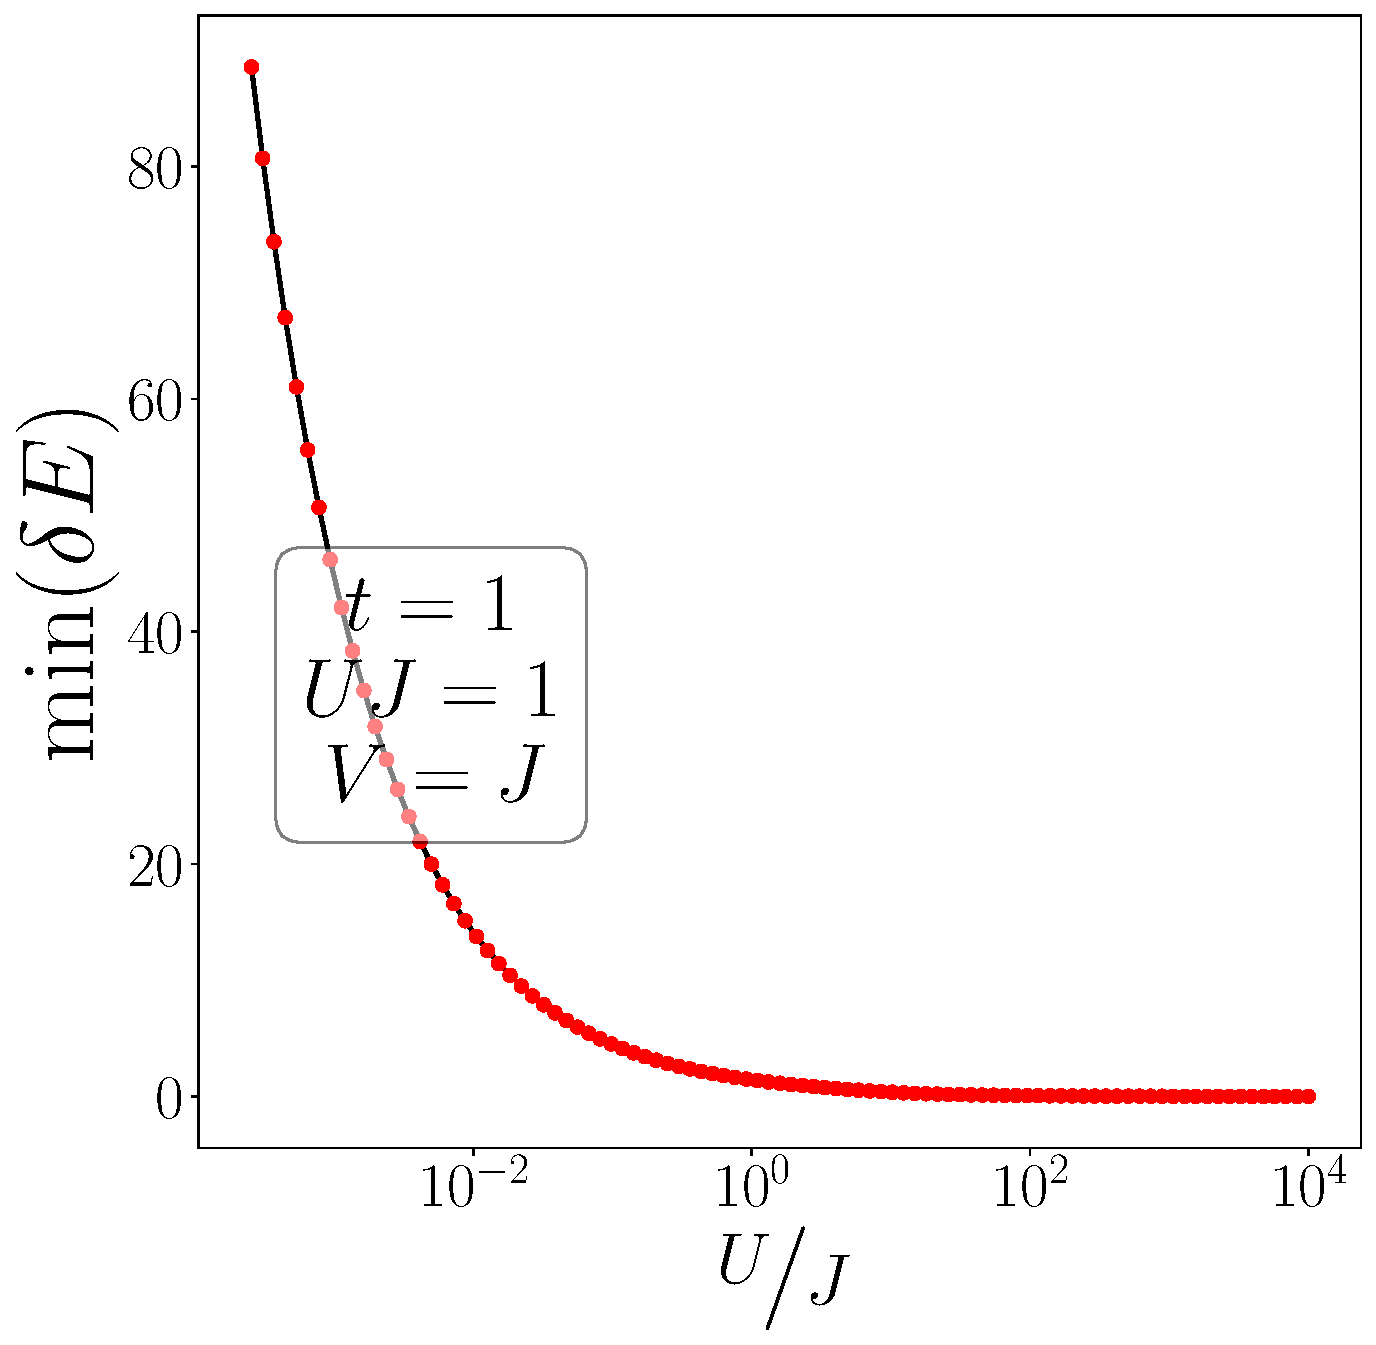
\includegraphics[width=0.3\textwidth]{figures/gap-t=1.000,J=1_over_U,V=J,N=4,U=0.016,100.000,95.pdf}
% \hspace*{\fill}
% 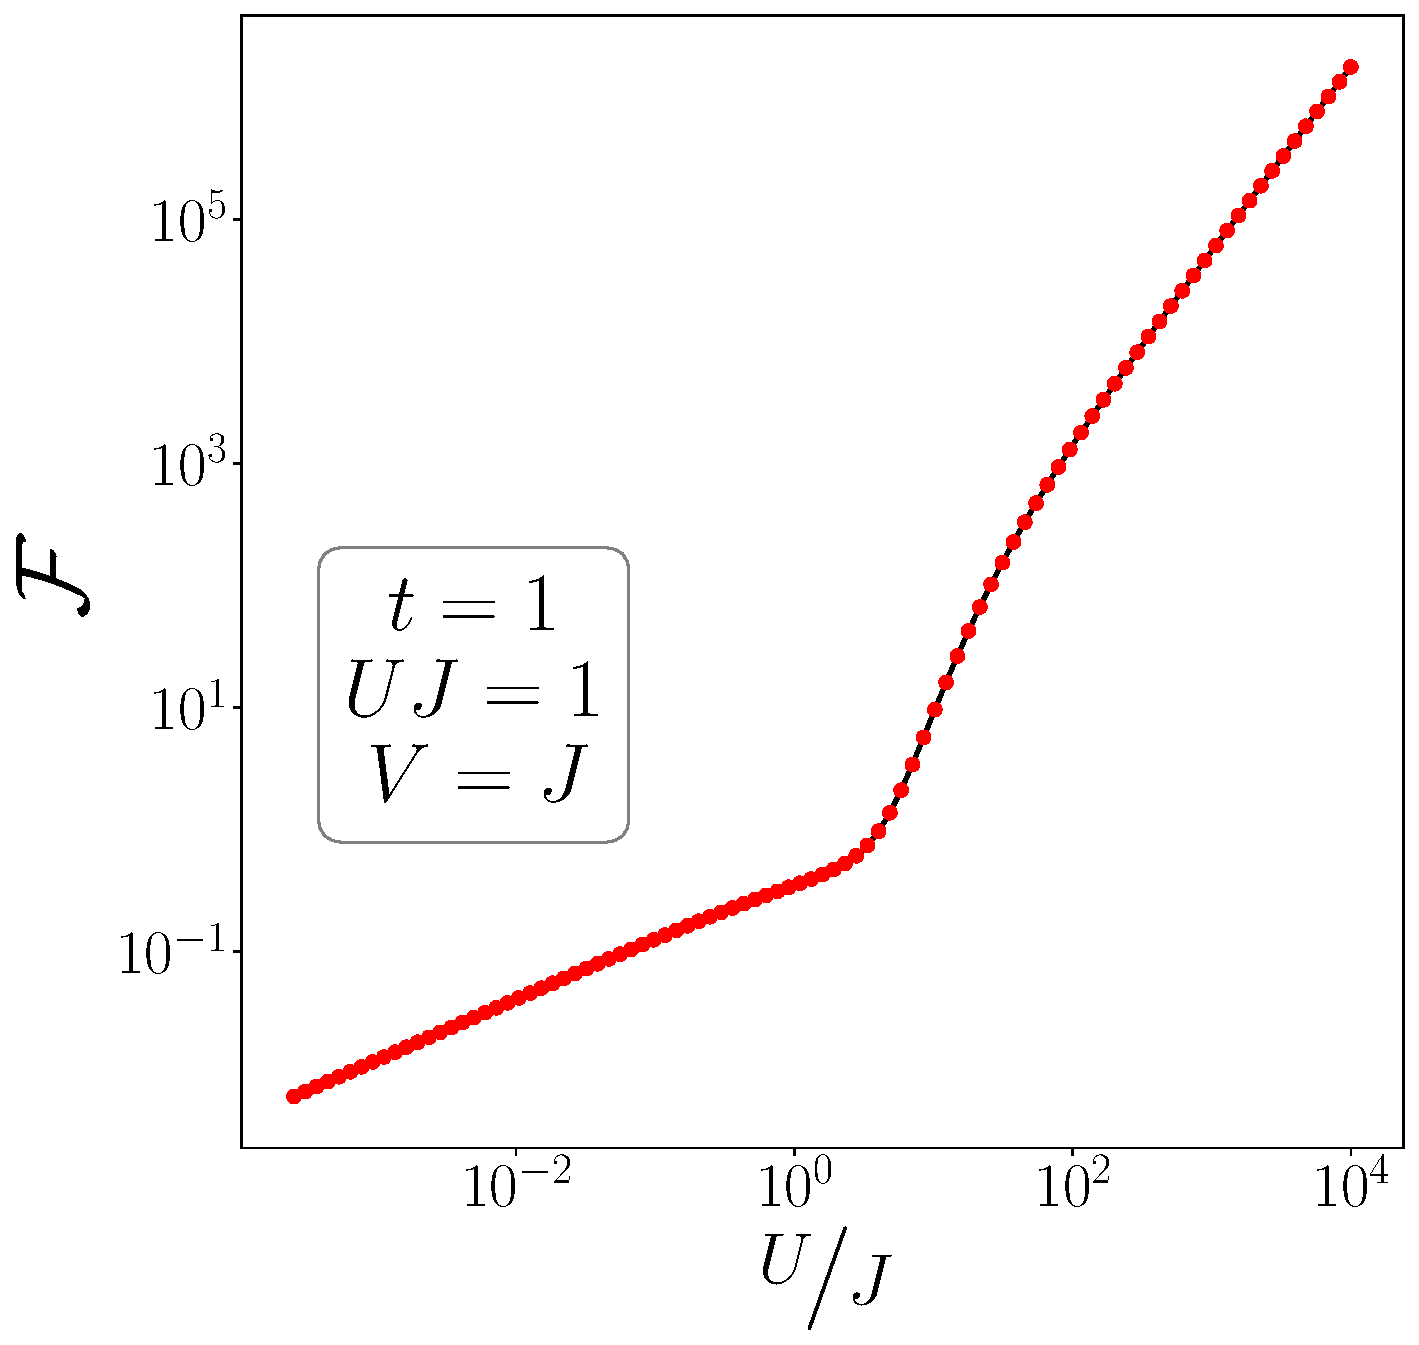
\includegraphics[width=0.3\textwidth]{figures/lfl-t=1.000,J=1_over_U,V=J,N=4,U=0.016,100.000,95.pdf}

% \focus{closing of gap},~ ~ ~ ~ breakdown of p. theory,~ ~ ~ ~  extremely \focus{correlated} LFL

% \vspace*{5pt}
% 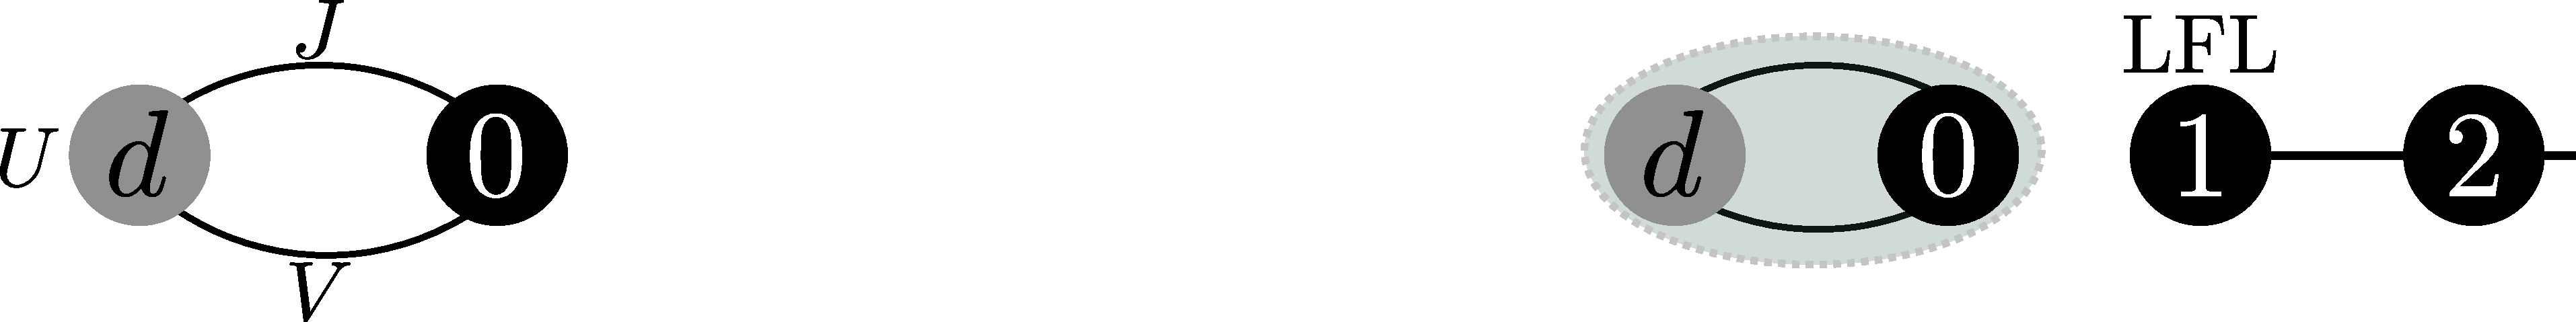
\includegraphics[width=0.95\textwidth]{figures/gap_lfl.pdf}
% }

% \end{frame}

% \begin{frame}[noframenumbering]{Destruction of Kondo cloud}
% \only<+>{
% \head{Mutual information within the Kondo cloud}
% \vspace*{20pt}
% \begin{center}
% 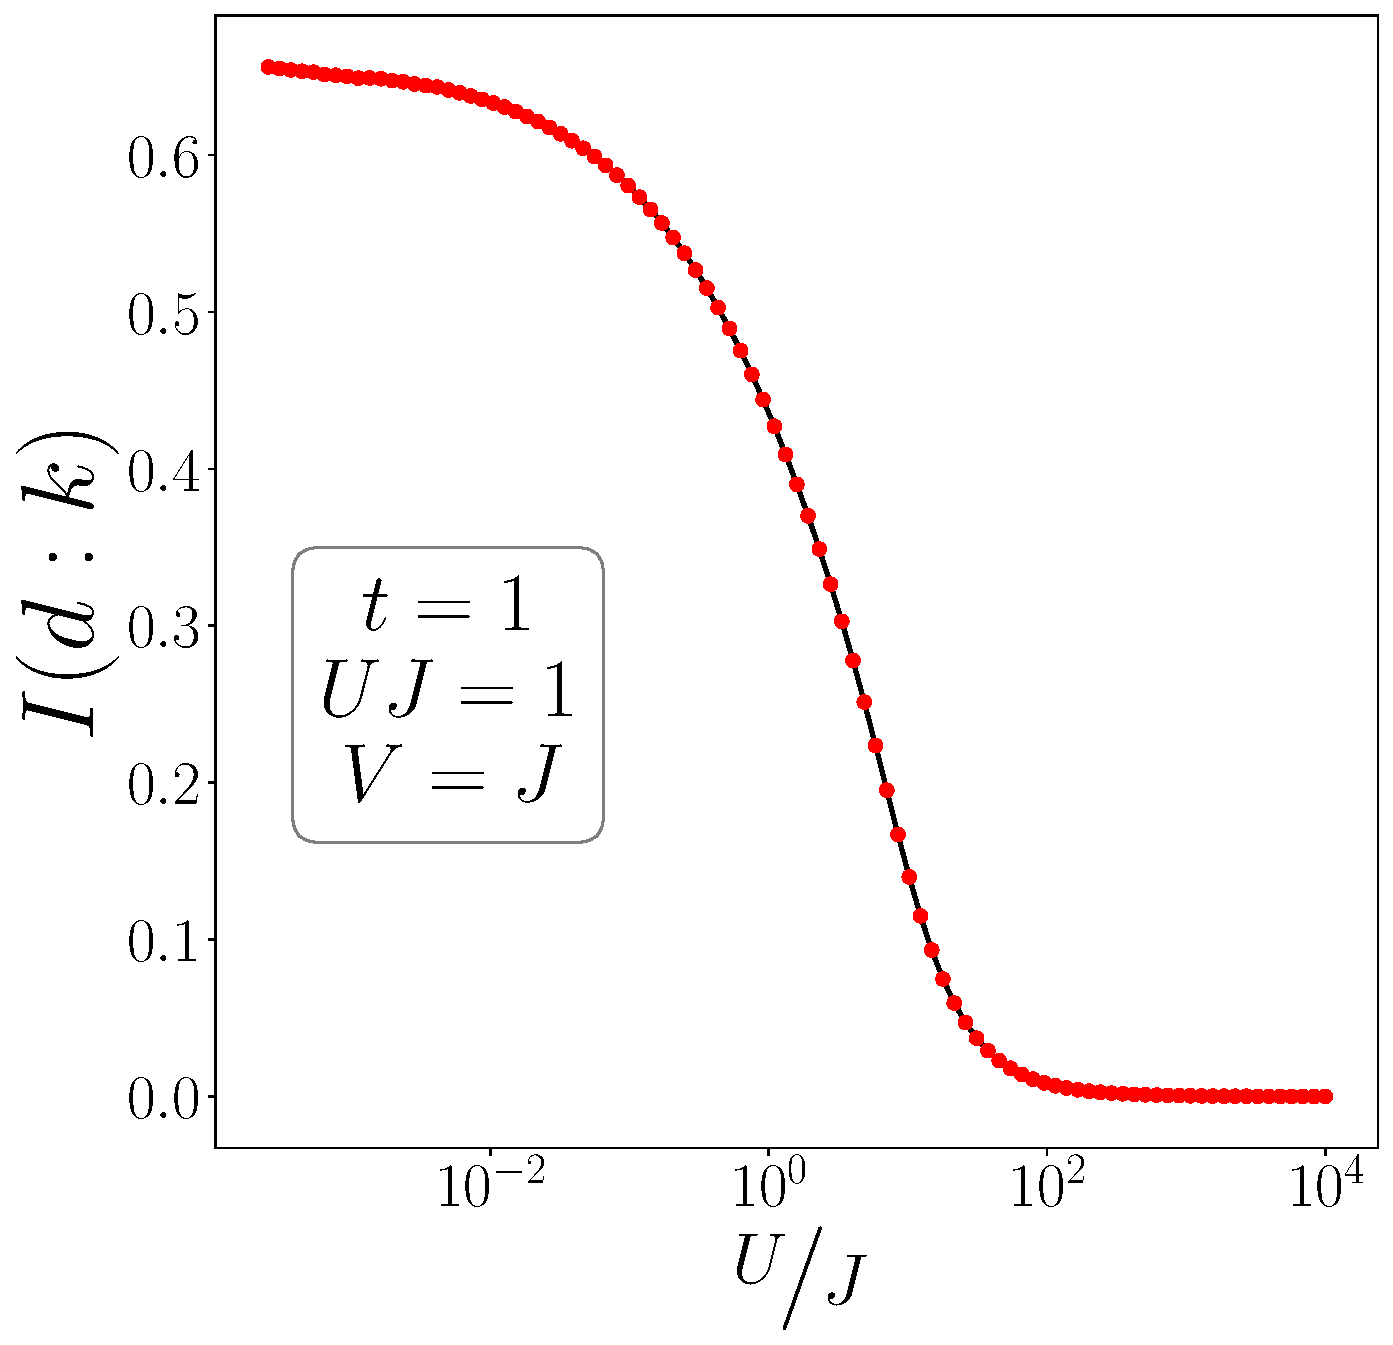
\includegraphics[width=0.35\textwidth]{figures/mi-dk-t=1.000,J=1_over_U,V=J,N=4,U=0.016,100.000,95.pdf}
% 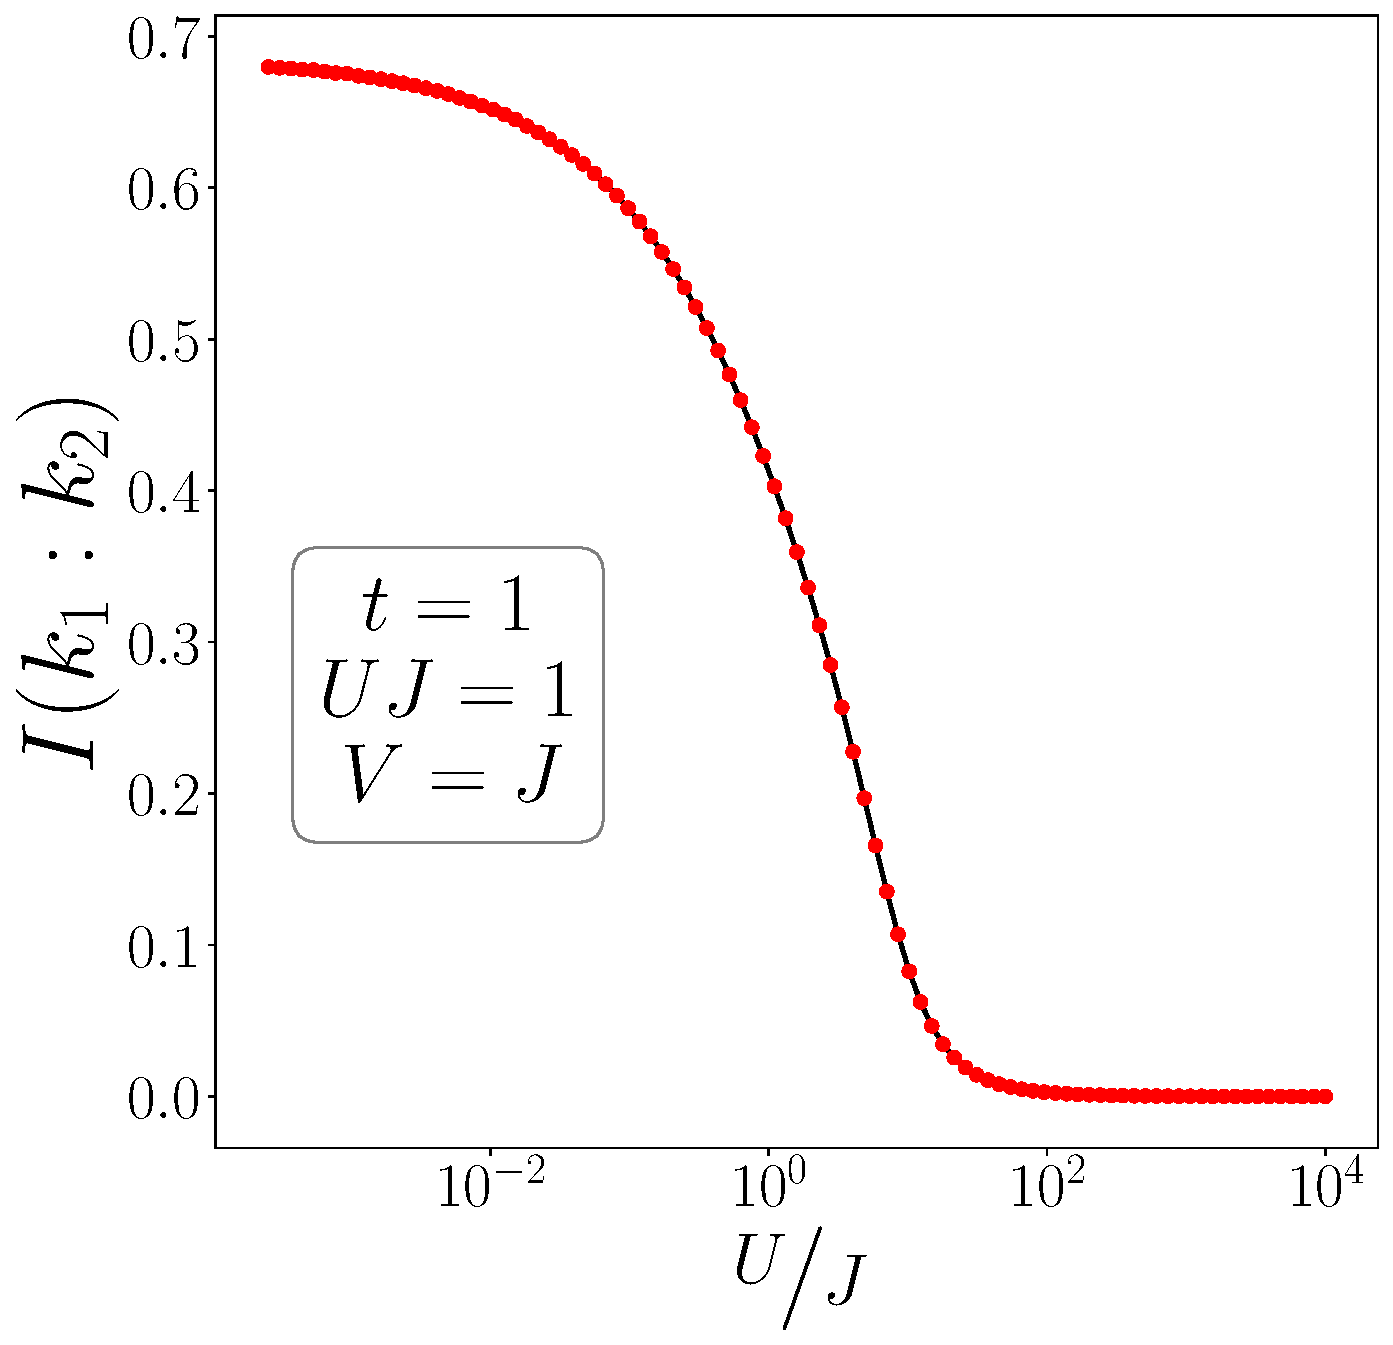
\includegraphics[width=0.35\textwidth]{figures/corr-k-t=1.000,J=1_over_U,V=J,N=4,U=0.016,100.000,95.pdf}
% \end{center}

% \vspace{-20pt}
% \begin{minipage}{0.7\textwidth}
% \begin{itemize}
% 	\item loss of spin-flip scattering and \focus{disappearance of Kondo cloud}
% \end{itemize}
% \end{minipage}
% \begin{minipage}{0.2\textwidth}
% 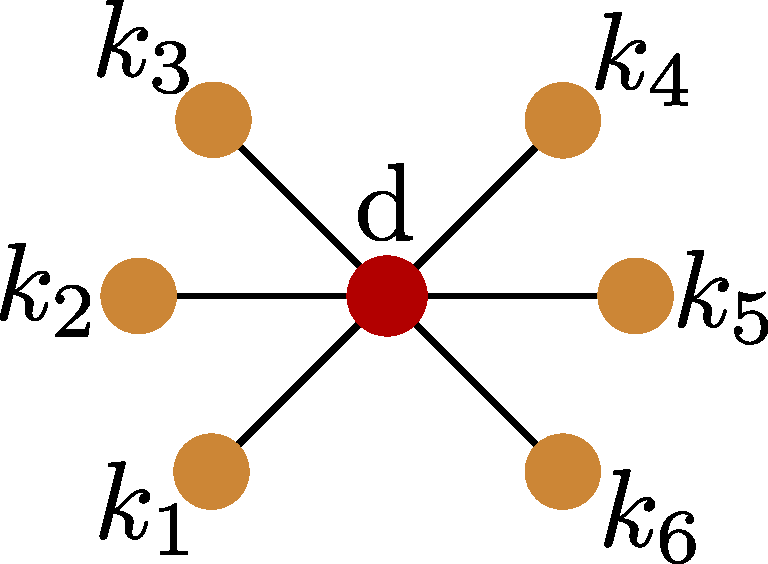
\includegraphics[width=\textwidth]{figures/seven_site2.pdf}
% \end{minipage}
% }

% \only<+>{
% \head{Many-particle correlations in \(k-\)space}
% \vspace*{20pt}

% \begin{center}
% 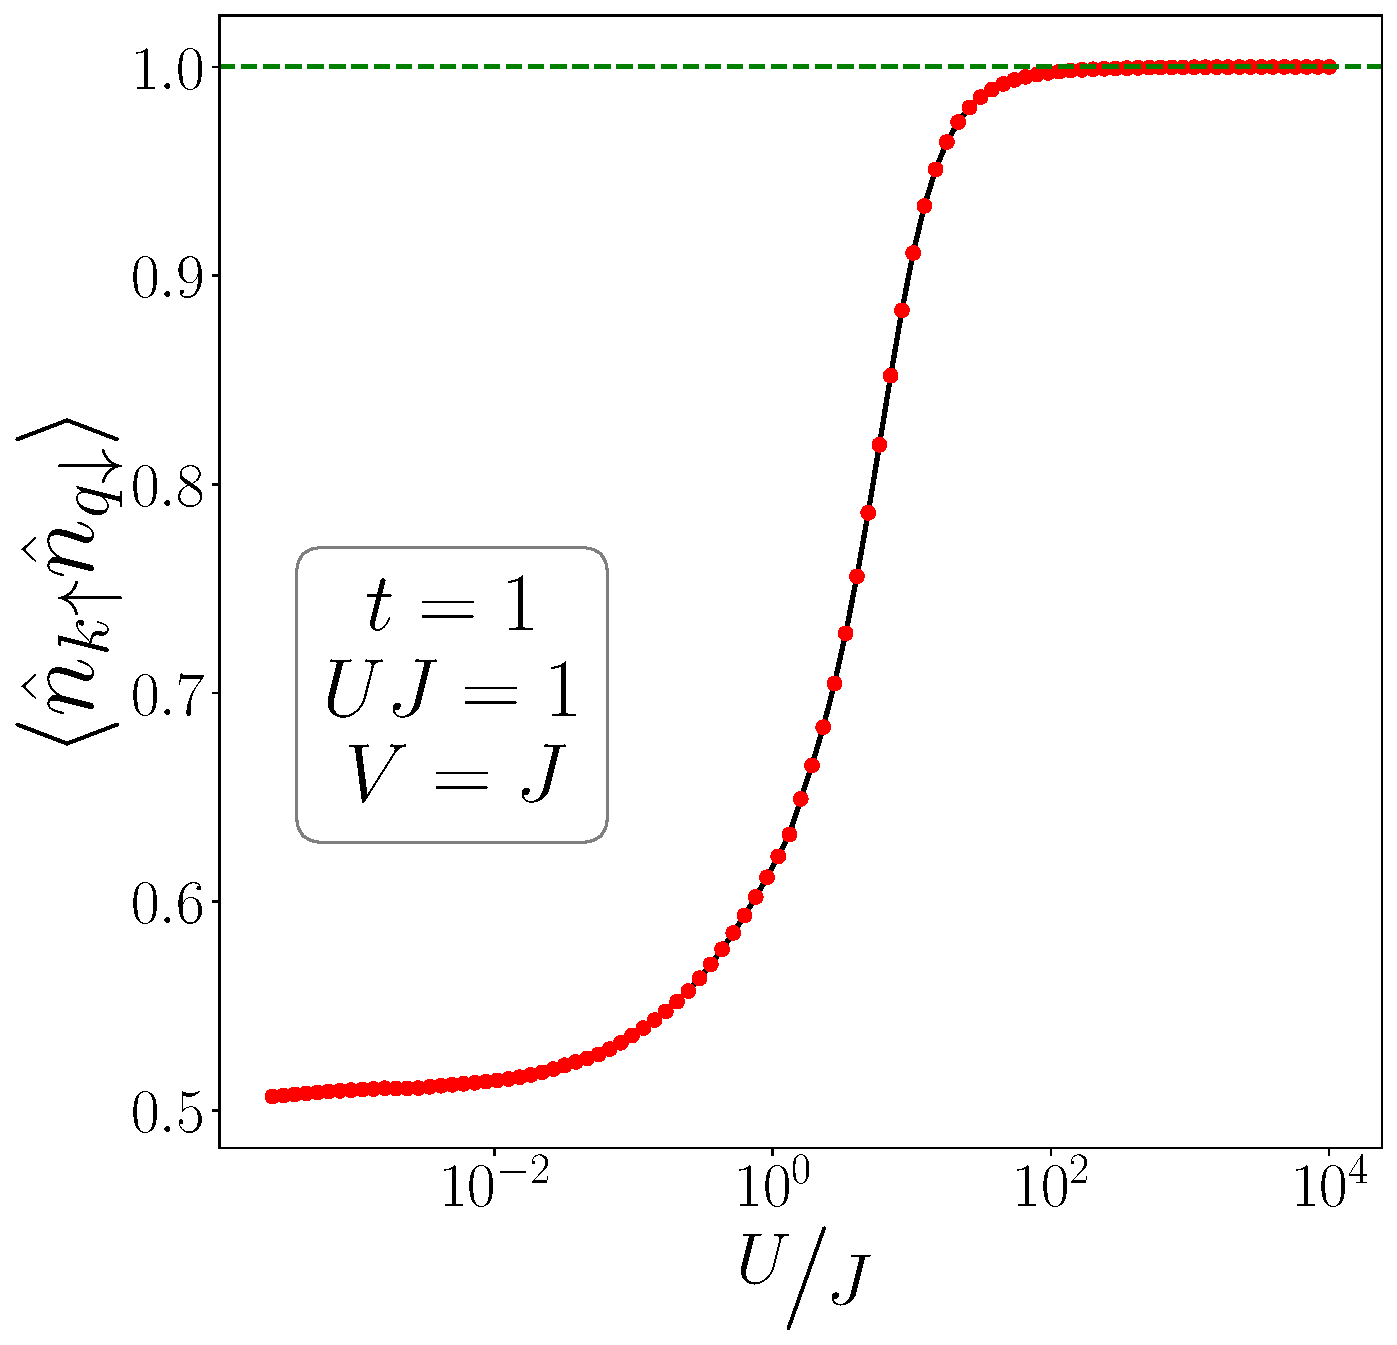
\includegraphics[width=0.35\textwidth]{figures/corr-k-diag-t=1.000,J=1_over_U,V=J,N=4,U=0.016,100.000,95.pdf}
% 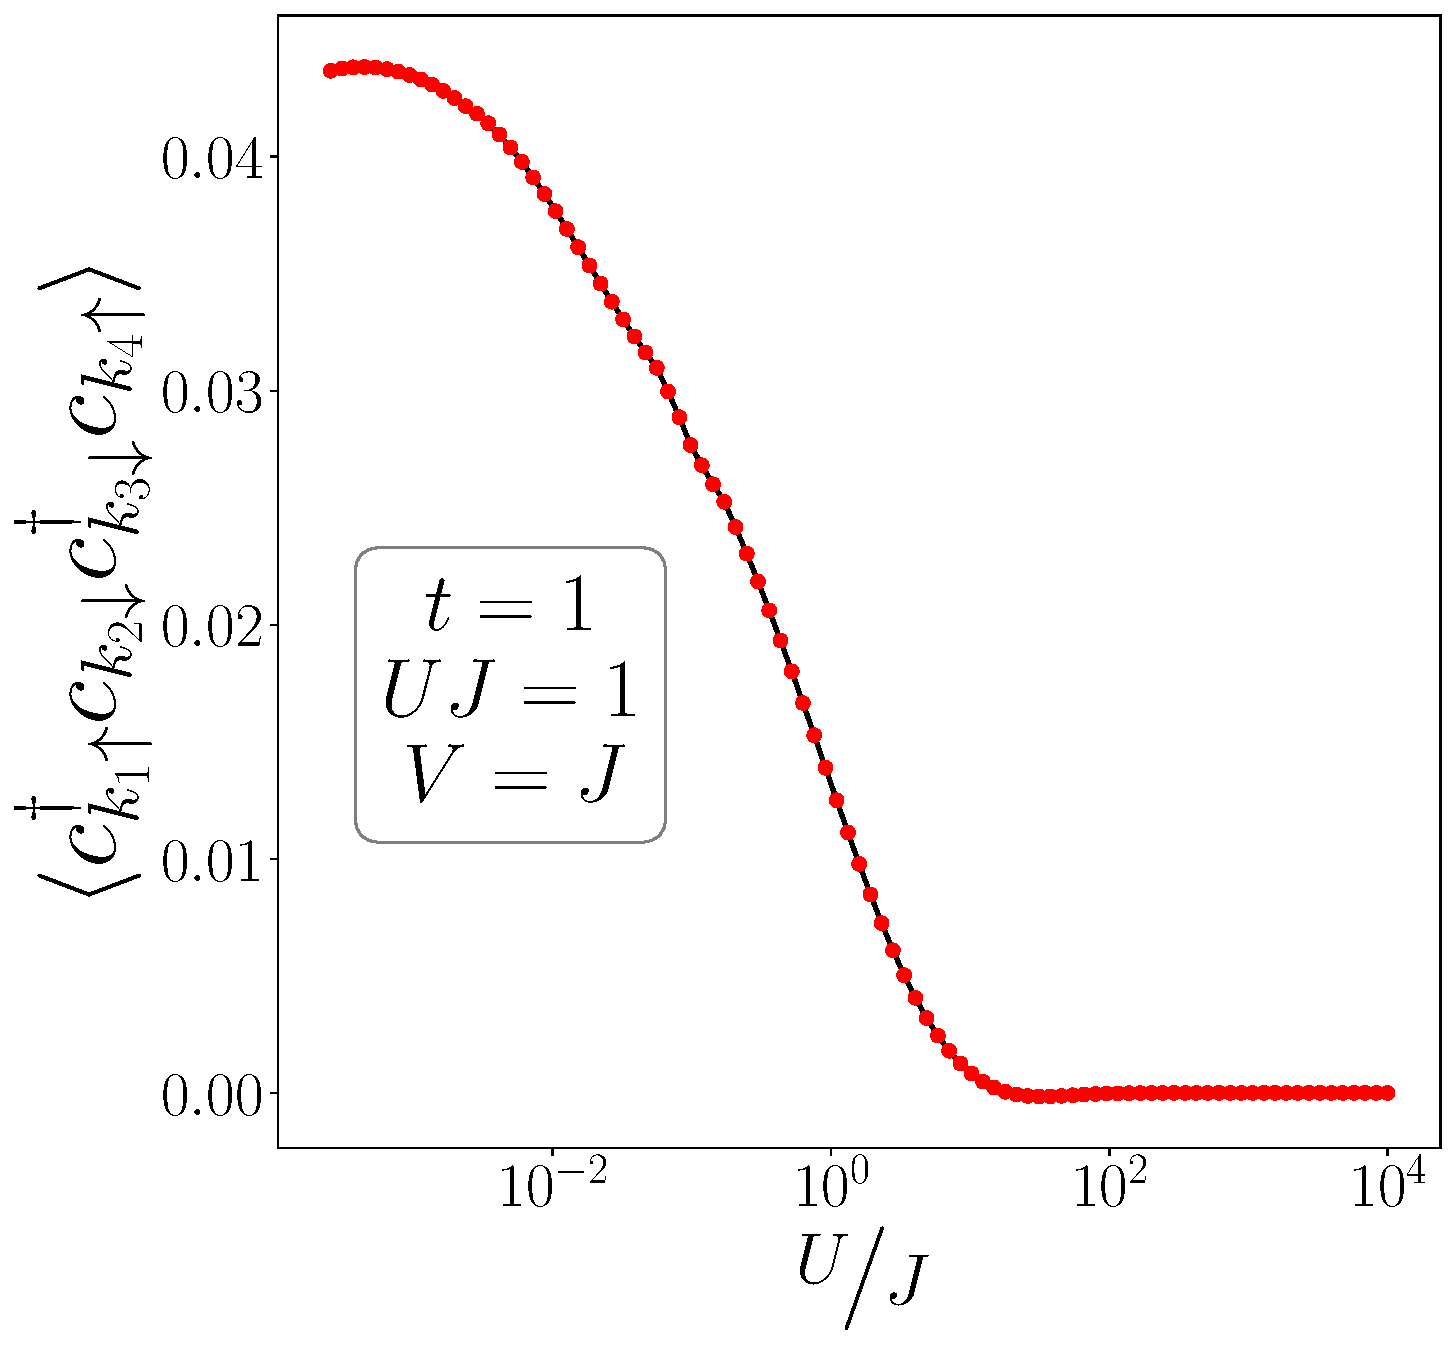
\includegraphics[width=0.37\textwidth]{figures/corr-k-od-t=1.000,J=1_over_U,V=J,N=4,U=0.016,100.000,95.pdf}
% \end{center}

% \vspace{-20pt}
% \begin{minipage}{0.7\textwidth}
% \begin{itemize}
% 	\item loss of entanglement within the K cloud, \focus{breakdown of screening}
% \end{itemize}
% \end{minipage}
% \begin{minipage}{0.2\textwidth}
% 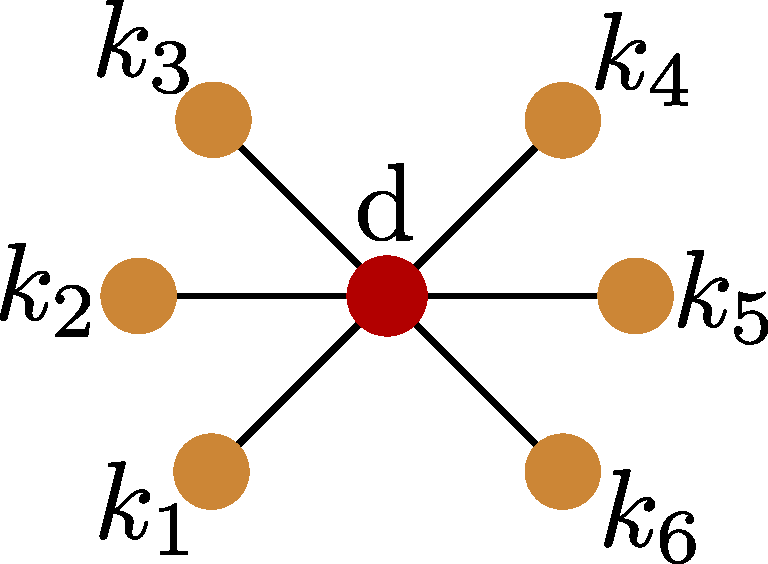
\includegraphics[width=\textwidth]{figures/seven_site2.pdf}
% \end{minipage}
% }
% \end{frame}

% \begin{frame}[noframenumbering]{Decoupling of impurity site from lattice}
% \only<+>{
% \head{Mutual information in real space}
% \begin{center}
% 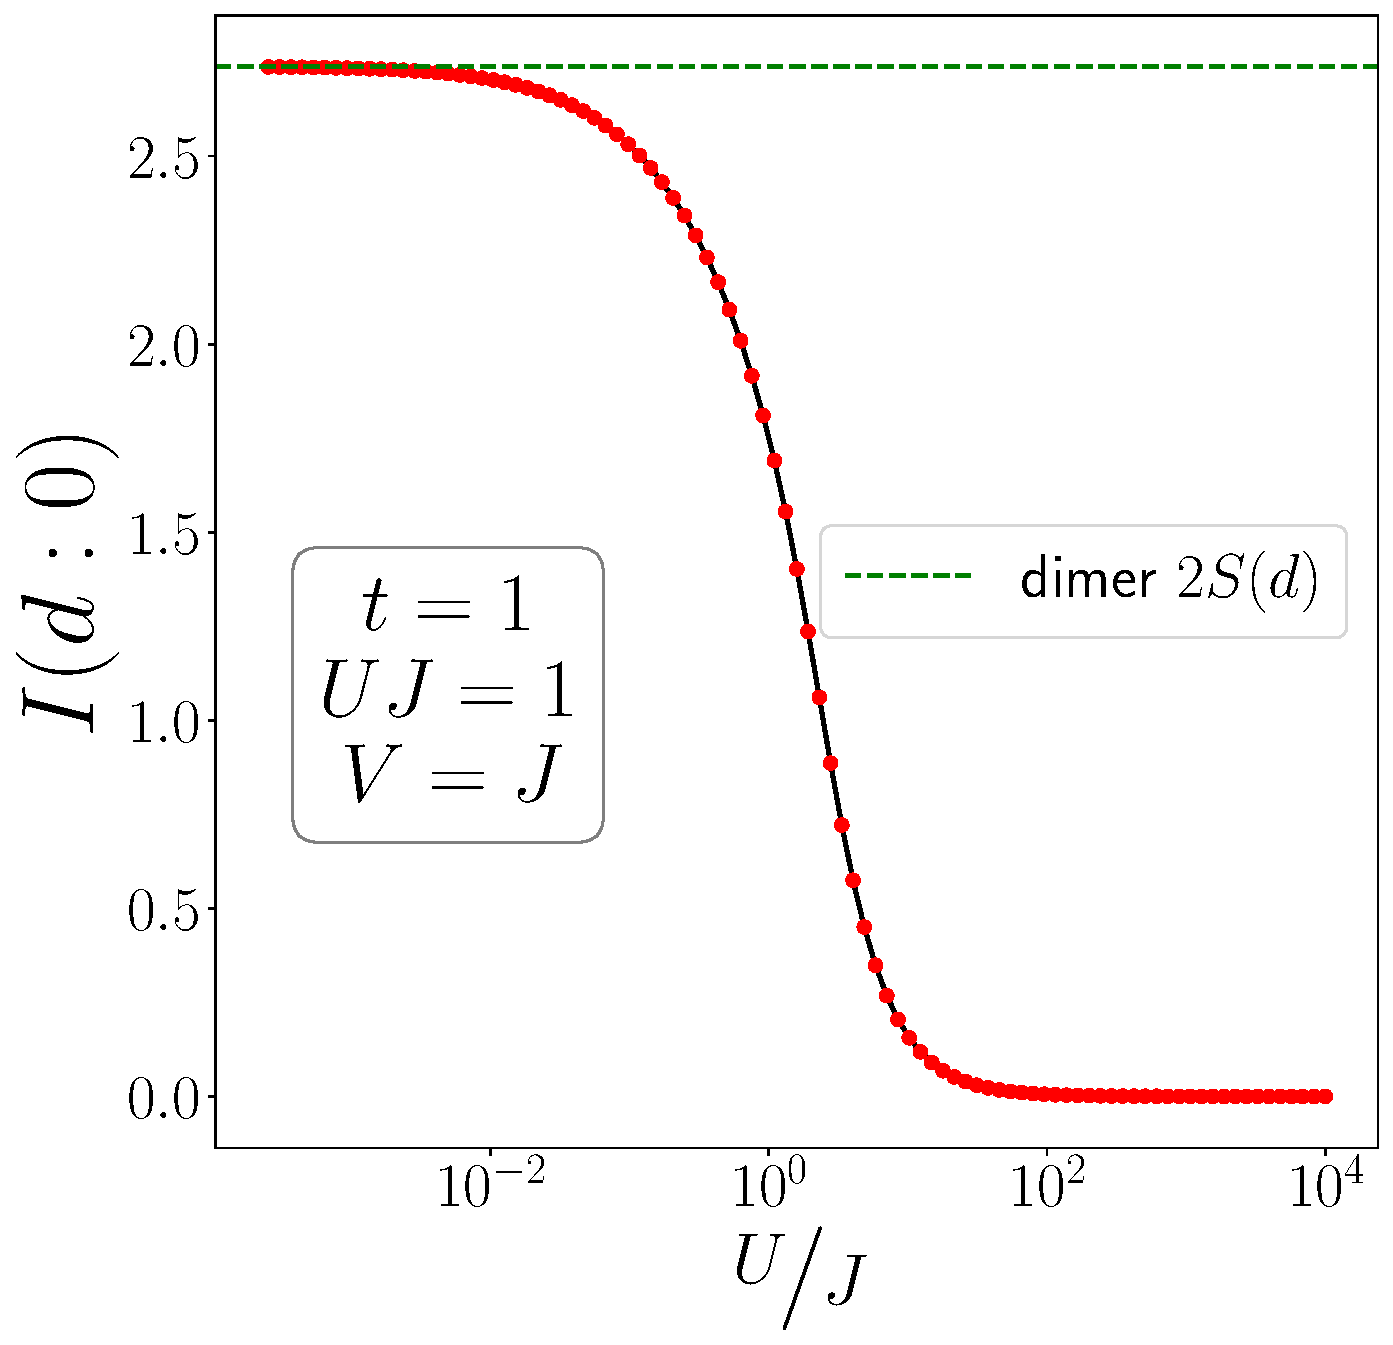
\includegraphics[width=0.32\textwidth]{figures/mi-d0-t=1.000,J=1_over_U,V=J,N=4,U=0.016,100.000,95.pdf}
% \hspace*{\fill}
% 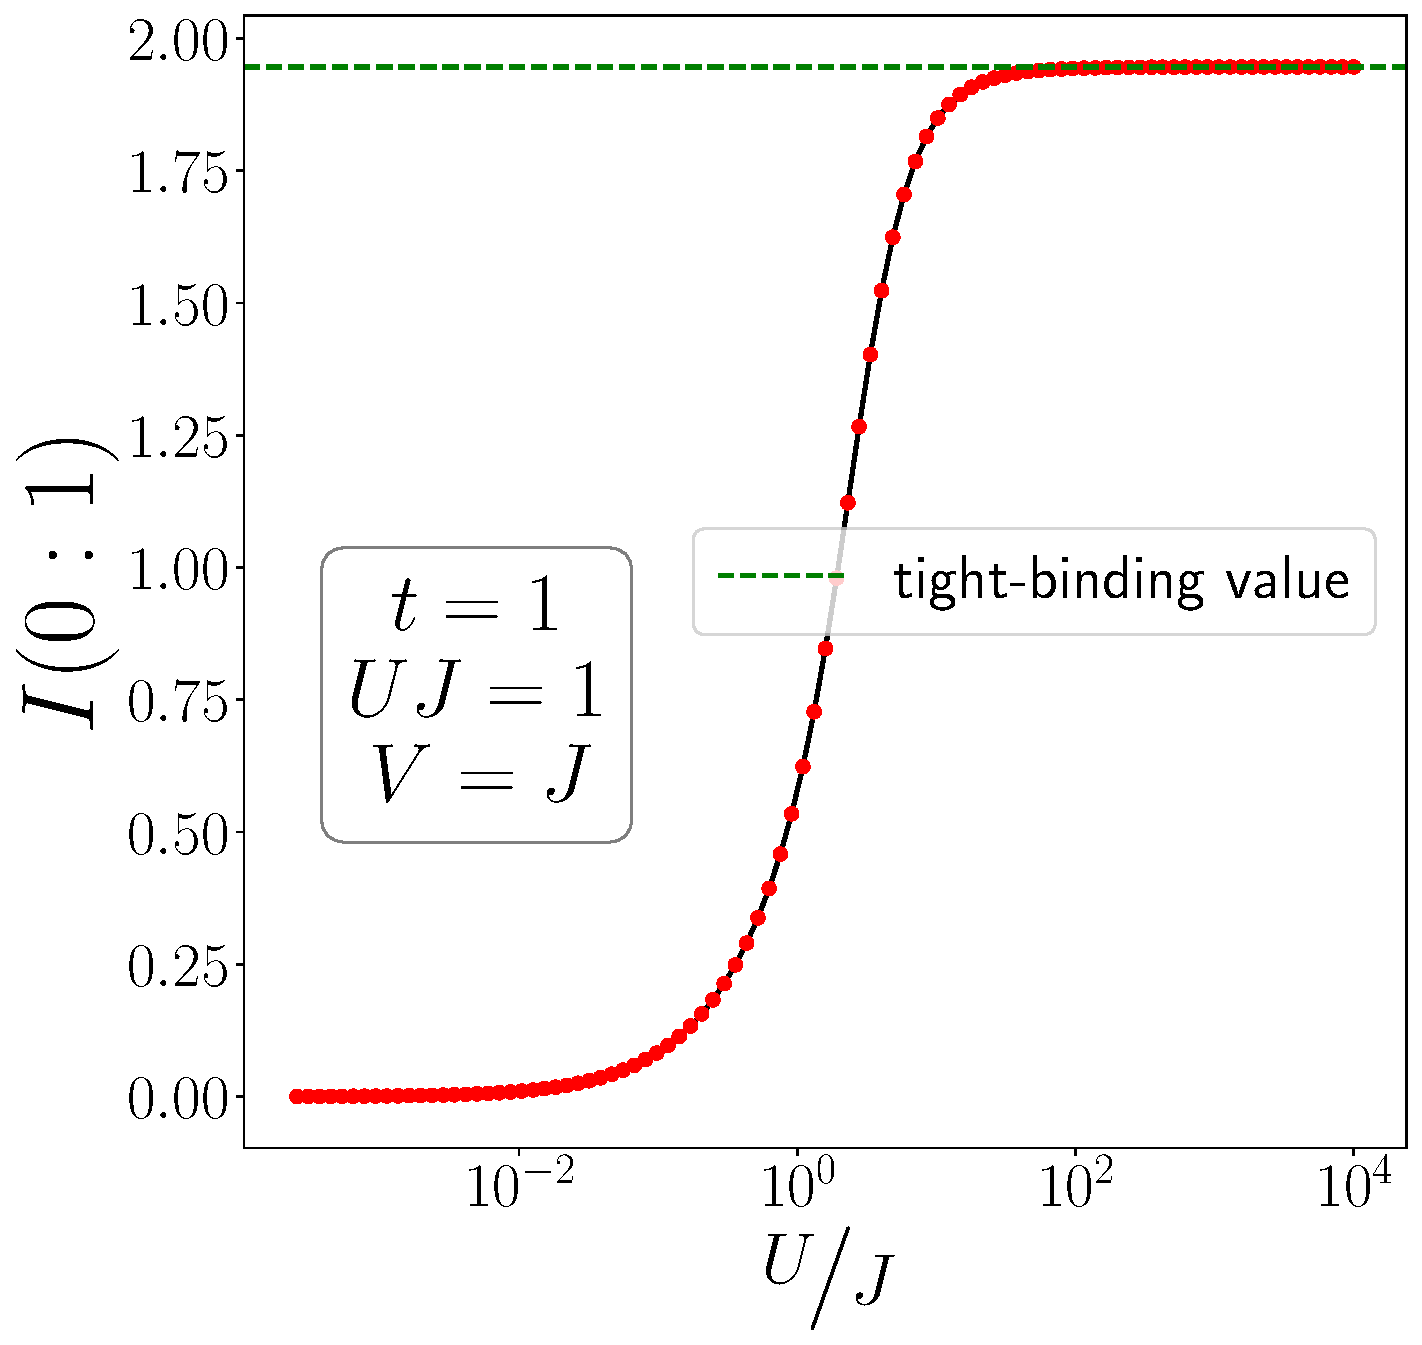
\includegraphics[width=0.32\textwidth]{figures/mi-01-t=1.000,J=1_over_U,V=J,N=4,U=0.016,100.000,95.pdf}
% \hspace*{\fill}
% 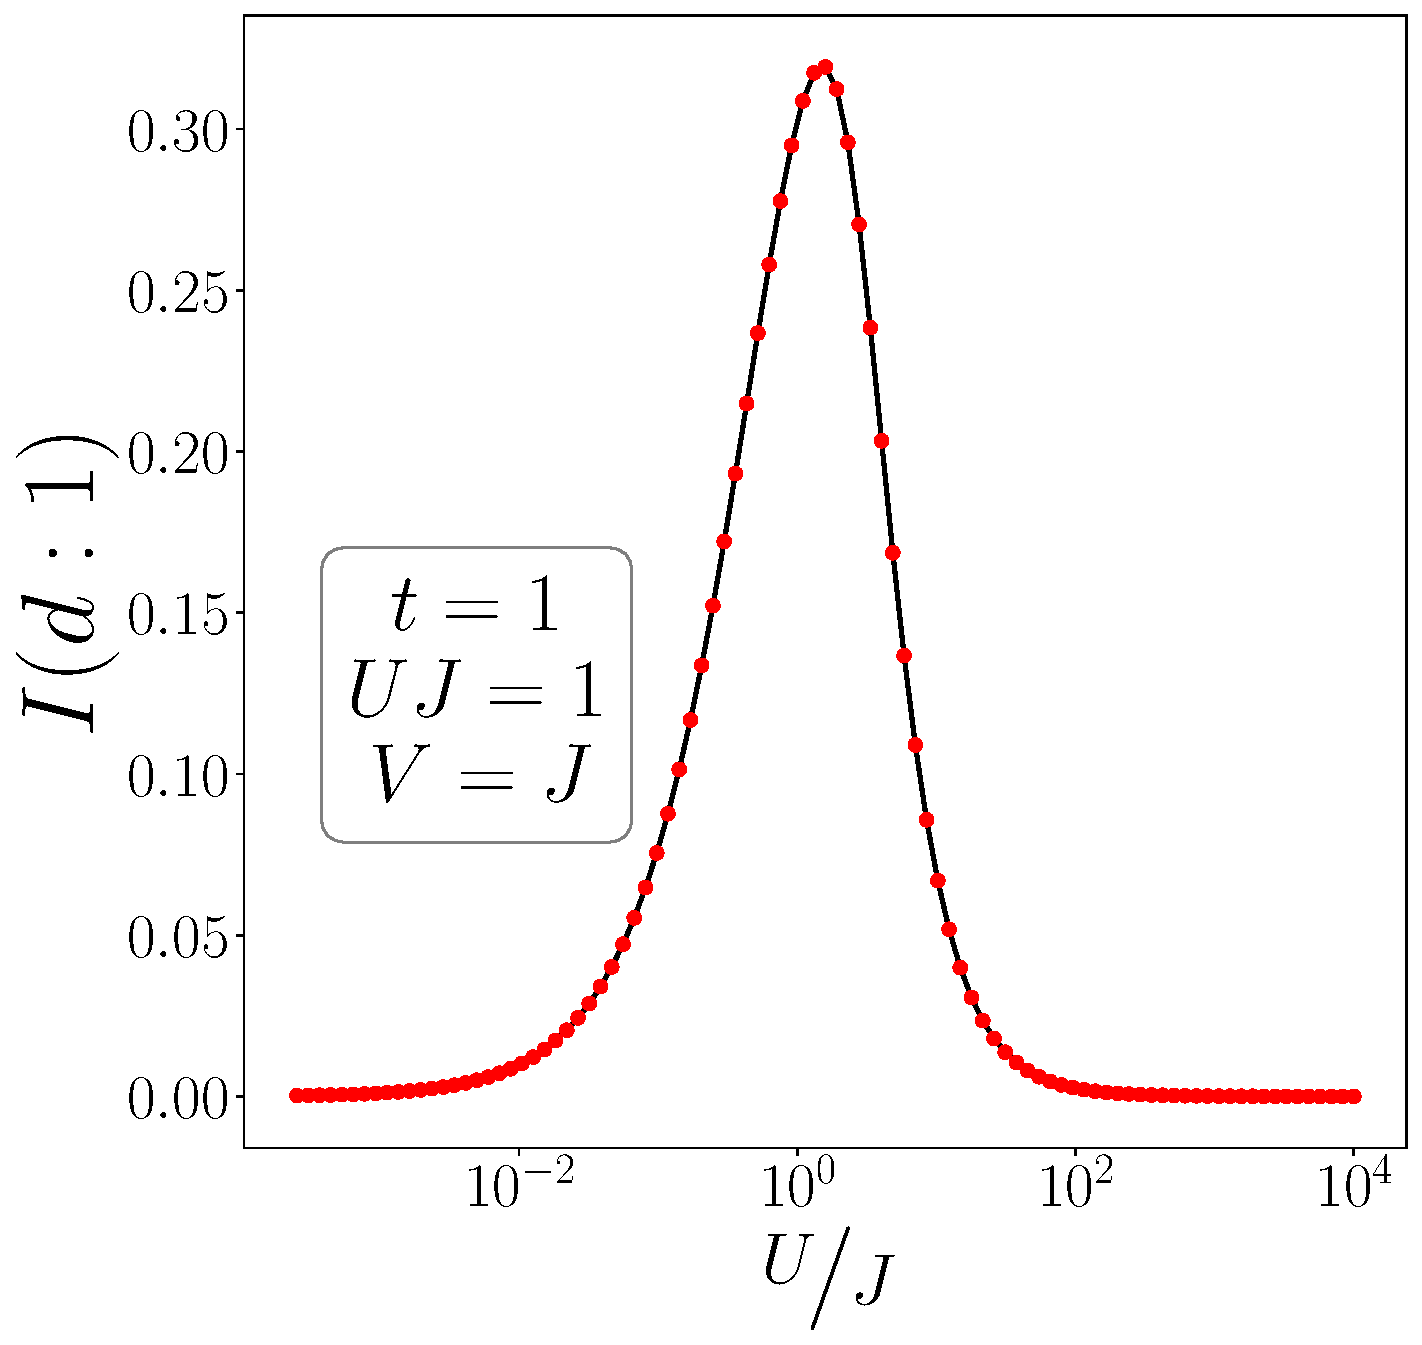
\includegraphics[width=0.32\textwidth]{figures/mi-d1-t=1.000,J=1_over_U,V=J,N=4,U=0.016,100.000,95.pdf}
% \end{center}

% \begin{minipage}{0.65\textwidth}
% \begin{itemize}
% 	\item \(d\) and \(0\) disentangle, \(0\) gets entangled with the lattice
% \end{itemize}
% \end{minipage}
% \begin{minipage}{0.29\textwidth}
% 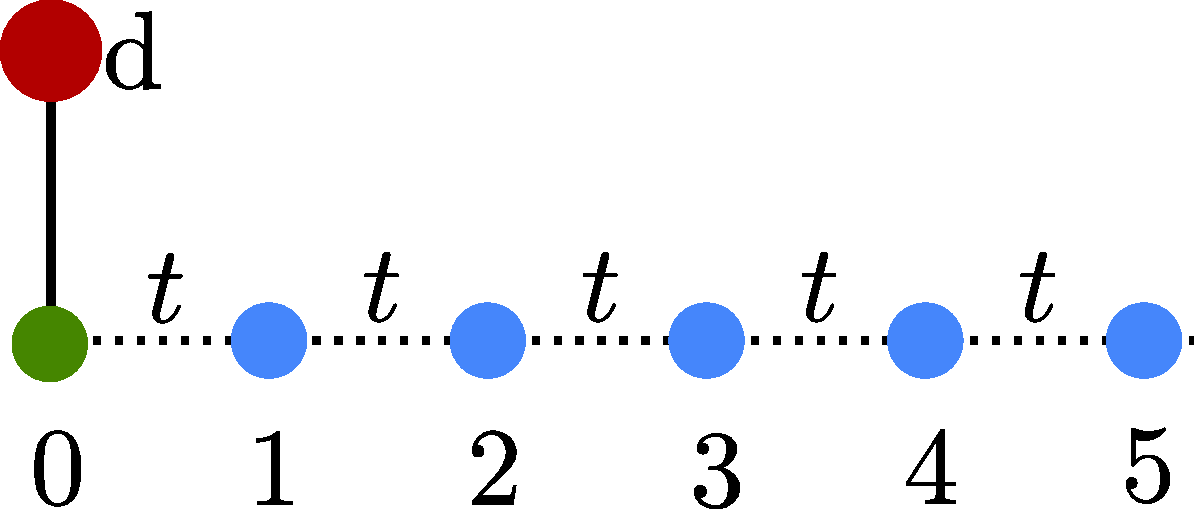
\includegraphics[width=\textwidth]{figures/seven_site.pdf}
% \end{minipage}
% }
% \only<+>{
% \head{Impurity entanglement entropy}
% \vspace*{20pt}
% \begin{center}
% 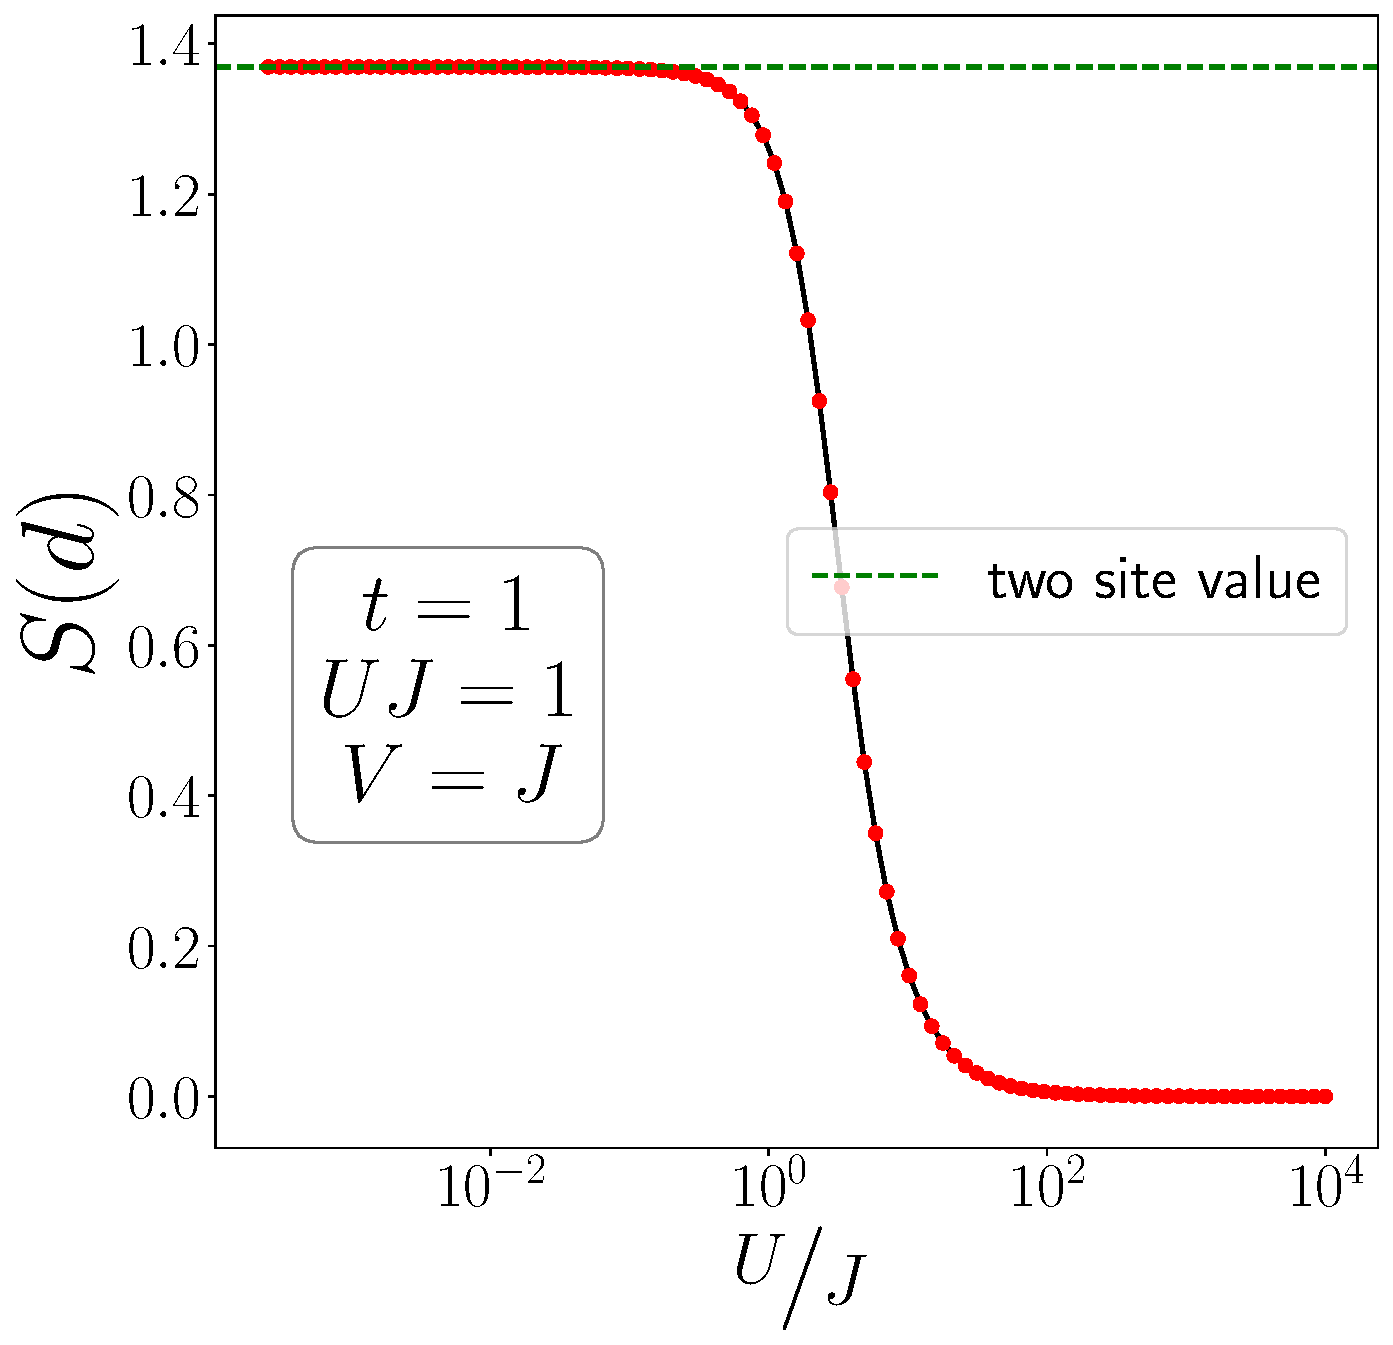
\includegraphics[width=0.35\textwidth]{figures/EE-d-t=1.000,J=1_over_U,V=J,N=4,U=0.016,100.000,95.pdf}
% \end{center}

% \begin{minipage}{0.65\textwidth}
% \begin{itemize}
% 	\item impurity site \focus{disentangles from the lattice}
% \end{itemize}
% \end{minipage}
% \begin{minipage}{0.29\textwidth}
% 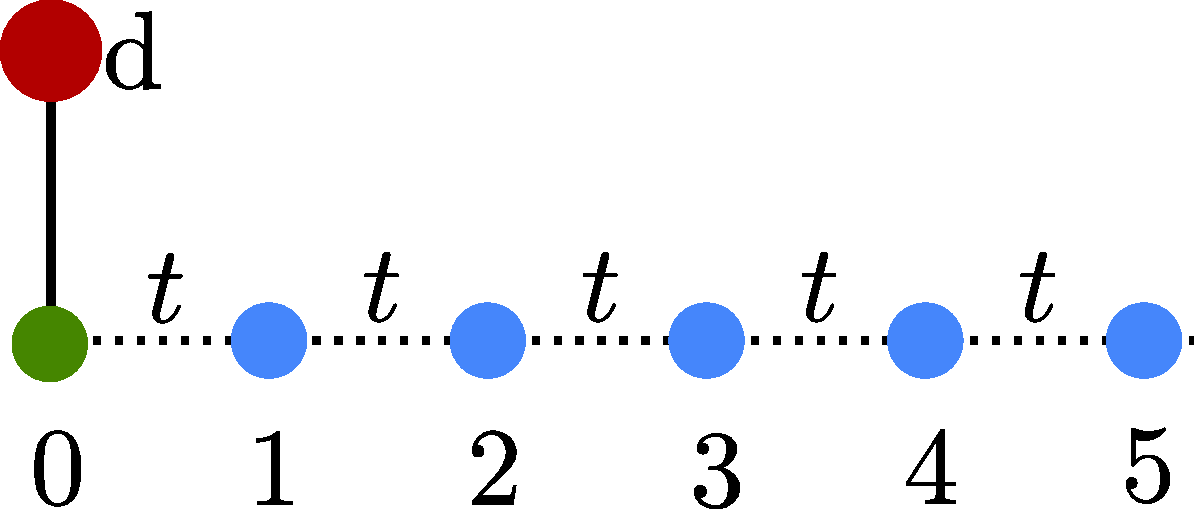
\includegraphics[width=\textwidth]{figures/seven_site.pdf}
% \end{minipage}
% }
% \only<+>{
% \head{Real space spin-spin correlations}
% \vspace*{20pt}
% \begin{center}
% 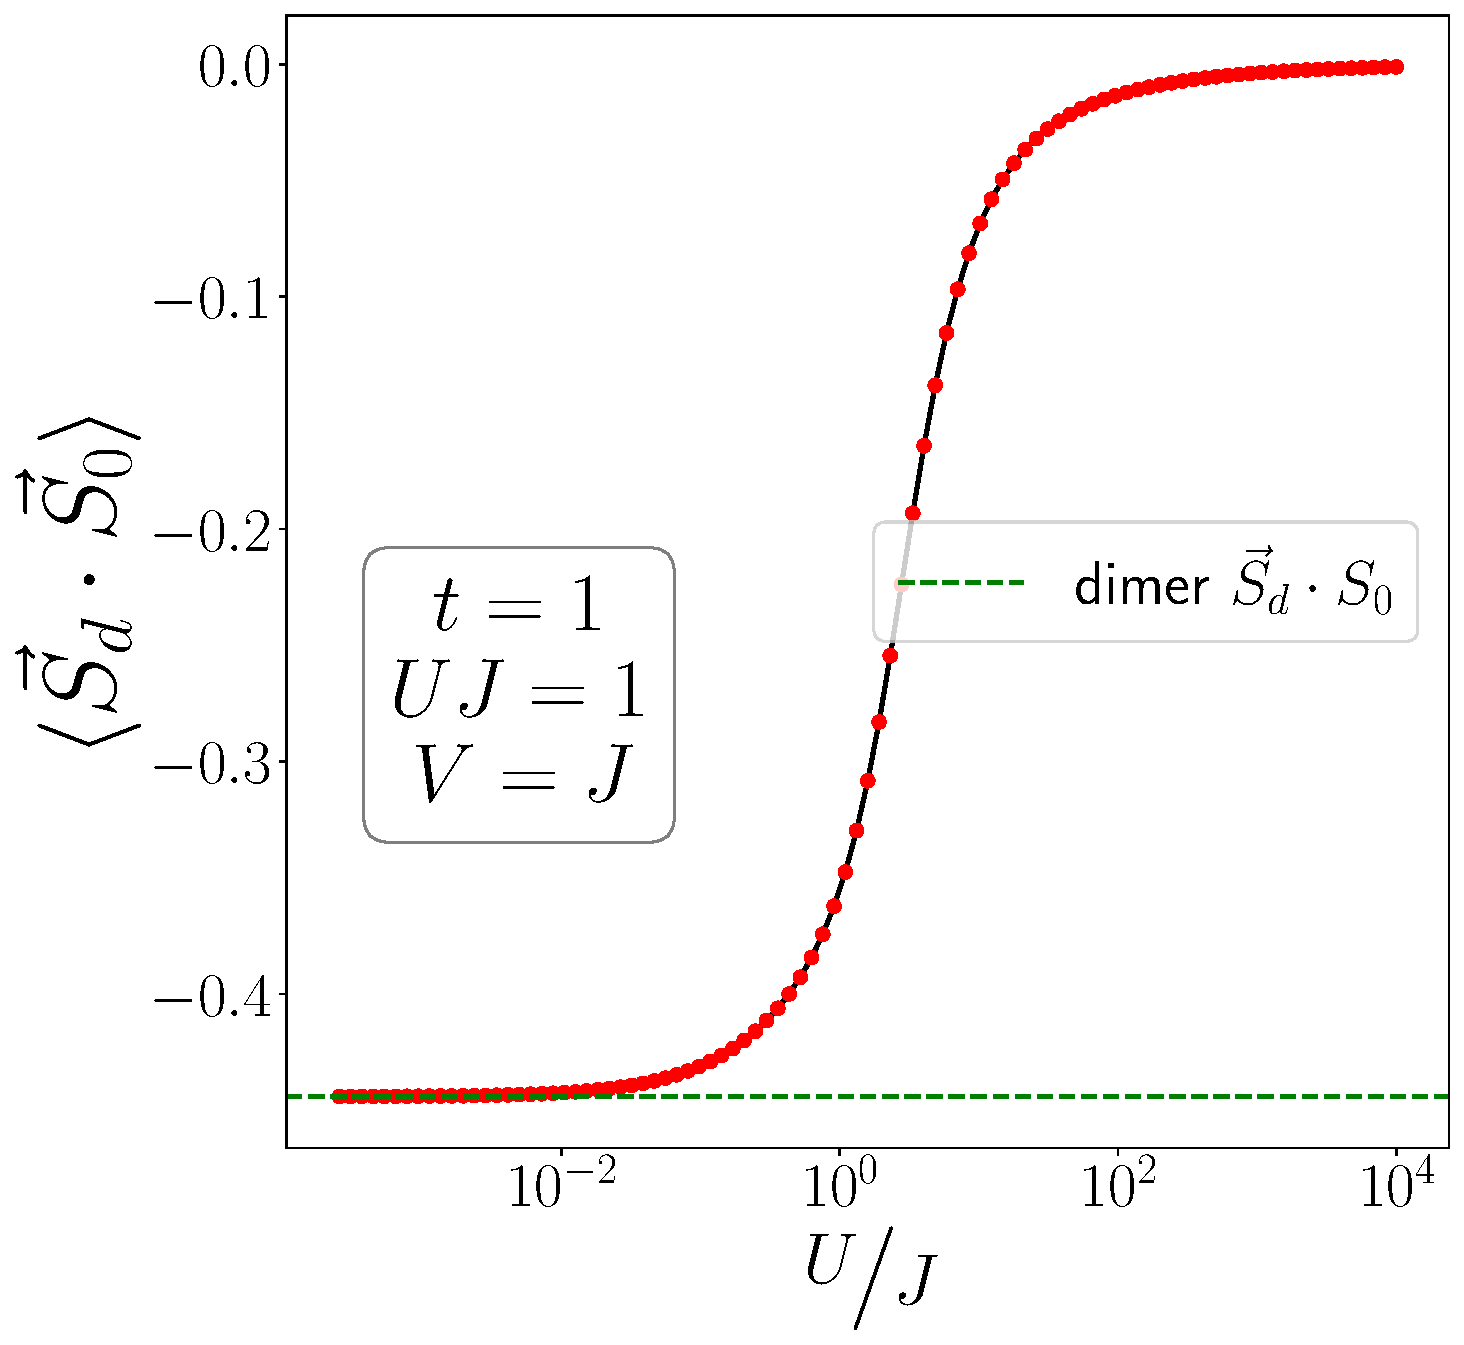
\includegraphics[width=0.32\textwidth]{figures/corr-d0-t=1.000,J=1_over_U,V=J,N=4,U=0.016,100.000,95.pdf}
% \hspace*{\fill}
% \includegraphics[width=0.32\textwidth]{figures/corr-d1-t=1.000,J=1_over_U,V=J,N=4,U=0.016,100.000,95.pdf}
% \hspace*{\fill}
% \includegraphics[width=0.32\textwidth]{figures/r-vec-corr-t=1.000,J=1_over_U,V=J,N=4,U=0.016,100.000,95.pdf}
% \end{center}

% \hspace*{-30pt}
% \begin{minipage}{0.73\textwidth}
% \begin{itemize}
% 	\item impurity\focus{ spin compensation vanishes} (loss of screening)
% 	\item Spin correlation between 0 and 1 increases
% \end{itemize}
% \end{minipage}
% \hspace{\fill}
% \begin{minipage}{0.29\textwidth}
% \includegraphics[width=\textwidth]{figures/seven_site.pdf}
% \end{minipage}
% }
% \only<+>{
% \head{Real space diagonal and off-diagonal correlations}
% \begin{center}
% \includegraphics[width=0.32\textwidth]{figures/r1p-t=1.000,J=1_over_U,V=J,N=4,U=0.016,100.000,95.pdf}
% \hspace*{\fill}
% \includegraphics[width=0.32\textwidth]{figures/r-od-t=1.000,J=1_over_U,V=J,N=4,U=0.016,100.000,95.pdf}
% \hspace*{\fill}
% \includegraphics[width=0.32\textwidth]{figures/r-ising-t=1.000,J=1_over_U,V=J,N=4,U=0.016,100.000,95.pdf}
% \hspace*{\fill}
% \end{center}

% \begin{minipage}{0.7\textwidth}
% \begin{itemize}
% 	\item \focus{Correlations between 0 and 1 increase}
% 	\item Result of tight-binding hopping \focus{breaking the singlet}
% \end{itemize}
% \end{minipage}
% \begin{minipage}{0.29\textwidth}
% \includegraphics[width=\textwidth]{figures/seven_site.pdf}
% \end{minipage}
% }
% \only<+>{
% \head{Variation of real-space correlations with distance}
% \vspace{20pt}
% \begin{center}
% \includegraphics[width=0.4\textwidth]{figures/corr-di-min-t=1.000,J=1_over_U,V=J,N=6,U=0.010,100.000,100.pdf}
% \hspace*{\fill}
% \includegraphics[width=0.45\textwidth]{figures/corr-di-max-t=1.000,J=1_over_U,V=J,N=6,U=0.010,100.000,100.pdf}
% \hspace*{\fill}
% \end{center}
% \vspace{-10pt}
% \begin{itemize}
% 	\item Correlations \focus{fall off with distance}
% 	\item Even sites are AFM in correlation, odd sites are FM
% \end{itemize}
% }
% \end{frame}

% \begin{frame}[noframenumbering]{Variation of Impurity Spectral Function}
% \centering
% \includegraphics[width=0.3\textwidth]{figures/spec-func-gen-siam-U_by_J=0.100.pdf}
% \includegraphics[width=0.3\textwidth]{figures/spec-func-gen-siam-U_by_J=9.000.pdf}
% \includegraphics[width=0.3\textwidth]{figures/spec-func-gen-siam-U_by_J=16.000.pdf}
% \includegraphics[width=0.3\textwidth]{figures/spec-func-gen-siam-U_by_J=20.250.pdf}
% \includegraphics[width=0.3\textwidth]{figures/spec-func-gen-siam-U_by_J=36.000.pdf}
% \includegraphics[width=0.3\textwidth]{figures/seven_site2.pdf}
% \end{frame}

\begin{frame}[noframenumbering]{What's happening?}
\includegraphics[width=0.9\textwidth]{figures/sc-lm.pdf}
\end{frame}


\begin{frame}[noframenumbering]{Auxiliary Model $\rightarrow$ bulk}
\includegraphics[width=0.9\textwidth]{figures/cloud_lattice.pdf}

\begin{itemize}
	\item At large \(J,V\), we have \focus{large overlapping} Kondo clouds (gray regions)
	\item As we go towards the local moment phase, the \focus{Kondo clouds shrink}
	\item At \(V,J \sim 0\), the Kondo \focus{length scale diverges} and the system becomes insulating
\end{itemize}

\end{frame}

\section{Discussions \& Further Work}
\begin{frame}[noframenumbering]{Discussions \& Further Work}
	\begin{itemize}[<+-|alert@+>]
		\item Rewinding the RG flow shows the \focus{decoupling} of the impurity site.
 		\item When used as an auxiliary model, this a \focus{metal-insulator transition}.
 		\item Stabilising the insulating phase under RG \focus{still remains to be done}.
 		\item For this, we will insert a \focus{Hubbard term on the zeroth site}, and check the RG flows.
	\end{itemize}
	\only<4>{
\includegraphics[width=0.6\textwidth]{figures/kondo_zeromode_Ubath.pdf}
	}
\end{frame}

% \section{Other measures of correlation in gen. SIAM}

% \begin{frame}[noframenumbering]{Real space correlations}

% \begin{center}
% \includegraphics[width=0.32\textwidth]{figures/r-opp-t=1.000,J=1_over_U,V=J,N=4,U=0.016,100.000,95.pdf}
% \includegraphics[width=0.32\textwidth]{figures/r-charge-t=1.000,J=1_over_U,V=J,N=4,U=0.016,100.000,95.pdf}
% \end{center}

% \end{frame}

% \begin{frame}[noframenumbering]{Real space correlations as functions of distance}

% \begin{center}
% \includegraphics[width=0.45\textwidth]{figures/corr-all-t=1.000,J=1_over_U,V=J,N=4,U=0.016,100.000,95.pdf}
% \includegraphics[width=0.45\textwidth]{figures/I-all-t=1.000,J=1_over_U,V=J,N=4,U=0.016,100.000,95.pdf}
% \end{center}

% \end{frame}

% \begin{frame}[noframenumbering]{Impurity spectral function (Gen. SIAM)}
% 	\centering
% 	\includegraphics[width=0.95\textwidth]{figures/gen_siam_spec_func.pdf}
% \end{frame}

% \section{Measures of correlation in pure SIAM}

% \begin{frame}[noframenumbering]{Breakdown of renormalised perturbation theory}

% \head{Perturbation parameter, zero mode gap and local FL strength}

% {
% \centering
% \includegraphics[width=0.3\textwidth]{figures/par-t=1.000,V=1_over_U,J=0,N=4,U=0.010,100.000,100.pdf}
% \hspace*{\fill}
% \includegraphics[width=0.3\textwidth]{figures/gap-t=1.000,V=1_over_U,J=0,N=4,U=0.010,100.000,100.pdf}
% \hspace*{\fill}
% \includegraphics[width=0.3\textwidth]{figures/lfl-t=1.000,V=1_over_U,J=0,N=4,U=0.010,100.000,100.pdf}
% }

% \end{frame}

% \begin{frame}[noframenumbering]{Destruction of Kondo cloud}
% \only<+>{
% \head{Mutual information within the Kondo cloud}

% \begin{center}
% \includegraphics[width=0.4\textwidth]{figures/mi-dk-t=1.000,V=1_over_U,J=0,N=4,U=0.010,100.000,100.pdf}
% \hspace*{\fill}
% \includegraphics[width=0.4\textwidth]{figures/corr-k-t=1.000,V=1_over_U,J=0,N=4,U=0.010,100.000,100.pdf}
% \end{center}
% }

% \only<+>{
% \head{Many-particle correlations in \(k-\)space}
% \begin{center}
% \includegraphics[width=0.4\textwidth]{figures/corr-k-diag-t=1.000,V=1_over_U,J=0,N=4,U=0.010,100.000,100.pdf}
% \hspace*{\fill}
% \includegraphics[width=0.4\textwidth]{figures/corr-k-od-t=1.000,V=1_over_U,J=0,N=4,U=0.010,100.000,100.pdf}
% \end{center}
% }
% \end{frame}

% \begin{frame}[noframenumbering]{Decoupling of impurity site from lattice}
% \only<+>{
% \head{Mutual information in real space}
% \begin{center}
% \includegraphics[width=0.32\textwidth]{figures/mi-d0-t=1.000,V=1_over_U,J=0,N=4,U=0.010,100.000,100.pdf}
% \hspace*{\fill}
% \includegraphics[width=0.32\textwidth]{figures/mi-01-t=1.000,V=1_over_U,J=0,N=4,U=0.010,100.000,100.pdf}
% \hspace*{\fill}
% \includegraphics[width=0.32\textwidth]{figures/mi-d1-t=1.000,V=1_over_U,J=0,N=4,U=0.010,100.000,100.pdf}
% \end{center}
% }
% \only<+>{
% \head{Impurity entanglement entropy}
% \begin{center}
% \includegraphics[width=0.4\textwidth]{figures/EE-d-t=1.000,V=1_over_U,J=0,N=4,U=0.010,100.000,100.pdf}
% \end{center}
% }
% \only<+>{
% \head{Real space spin-spin correlations}
% \begin{center}
% \includegraphics[width=0.32\textwidth]{figures/corr-d0-t=1.000,V=1_over_U,J=0,N=4,U=0.010,100.000,100.pdf}
% \hspace*{\fill}
% \includegraphics[width=0.32\textwidth]{figures/corr-d1-t=1.000,V=1_over_U,J=0,N=4,U=0.010,100.000,100.pdf}
% \hspace*{\fill}
% \includegraphics[width=0.32\textwidth]{figures/r-vec-corr-t=1.000,V=1_over_U,J=0,N=4,U=0.010,100.000,100.pdf}
% \end{center}
% }
% \only<+>{
% \head{Real space off-diagonal 1-particle and 2-particle correlations}
% \begin{center}
% \includegraphics[width=0.4\textwidth]{figures/r1p-t=1.000,V=1_over_U,J=0,N=4,U=0.010,100.000,100.pdf}
% \hspace*{\fill}
% \includegraphics[width=0.4\textwidth]{figures/r-od-t=1.000,V=1_over_U,J=0,N=4,U=0.010,100.000,100.pdf}
% \hspace*{\fill}
% \end{center}
% }
% \only<+>{
% \head{Real space diagonal correlations}
% \begin{center}
% \includegraphics[width=0.4\textwidth]{figures/r-par-t=1.000,V=1_over_U,J=0,N=4,U=0.010,100.000,100.pdf}
% \hspace*{\fill}
% \includegraphics[width=0.4\textwidth]{figures/r-ising-t=1.000,V=1_over_U,J=0,N=4,U=0.010,100.000,100.pdf}
% \hspace*{\fill}
% \end{center}
% }
% \only<+>{
% \head{Variation of real-space correlations with distance}
% \begin{center}
% \includegraphics[width=0.4\textwidth]{figures/corr-di-min-t=1.000,V=1_over_U,J=0,N=4,U=0.010,100.000,100.pdf}
% \hspace*{\fill}
% \includegraphics[width=0.4\textwidth]{figures/corr-di-max-t=1.000,V=1_over_U,J=0,N=4,U=0.010,100.000,100.pdf}
% \hspace*{\fill}
% \end{center}
% }
% \end{frame}

% \begin{frame}[noframenumbering]{Form of Kondo cloud Hamiltonian}
	
% \centering
% \[H_\text{eff}=2H^{*}_{0} ~+~ \frac{2}{J^*}{H^{*}_{0}}^2 ~+~ \sum_{1234}V_{1234}c^\dagger_{{k_4} \uparrow}c^\dagger_{{k_3} \downarrow}c_{{k_2} \downarrow}c_{{k_1} \uparrow}\label{eff_Ham_Kondo}\]
% \[V_{1234} = \left( \epsilon_{k_1} - \epsilon_{k_3} \right)\left[1 - \frac{2}{J^*}\left(\epsilon_{k_3} - \epsilon_{{k_1}} + \epsilon_{{k_2}} + \epsilon_{{k_4}}\right)\right]\]

% \begin{itemize}
% 	\item Mixture of \focus{Fermi liquid} and \focus{two-particle off-diagonal scattering term}
% 		\vspace*{\fill}
% 	\item Fermi liquid part: \focus{result of Ising scattering}
% 		\vspace*{\fill}
% 	\item 2P off-diagonal term: \focus{Non-Fermi liquid} in character - \focus{result of spin-flip scattering}
% 		\vspace*{\fill}
% 	\item NFL part \focus{leads to screening} and formation of singlet
% \end{itemize}

% \end{frame}
\end{document}
